\chapter{Appendix D - Machine Learning}

\section{Test Conditions and Data Summary}
\FloatBarrier

The following charts show trends in precipitation, ambient pressure, cloud cover, dew, and light level over the course of our two month MassDEP co-location test.

\begin{table}[H]
\centering
\begin{tabular}{lllllllll}
\\
\\
\toprule
Weather Type & \# Hours During Test \\
\midrule
clear hours & 901 \\
partly cloudy hours & 292 \\
cloudy hours & 103 \\
raining hours & 96 \\
windy hours & 25 \\
foggy hours & 11 \\
\bottomrule
\end{tabular}
\label{tab:as1_co_randomforest_features}
\caption{Most Frequent Weather During Co-location Test}
\end{table}


\begin{figure}[htb]
 	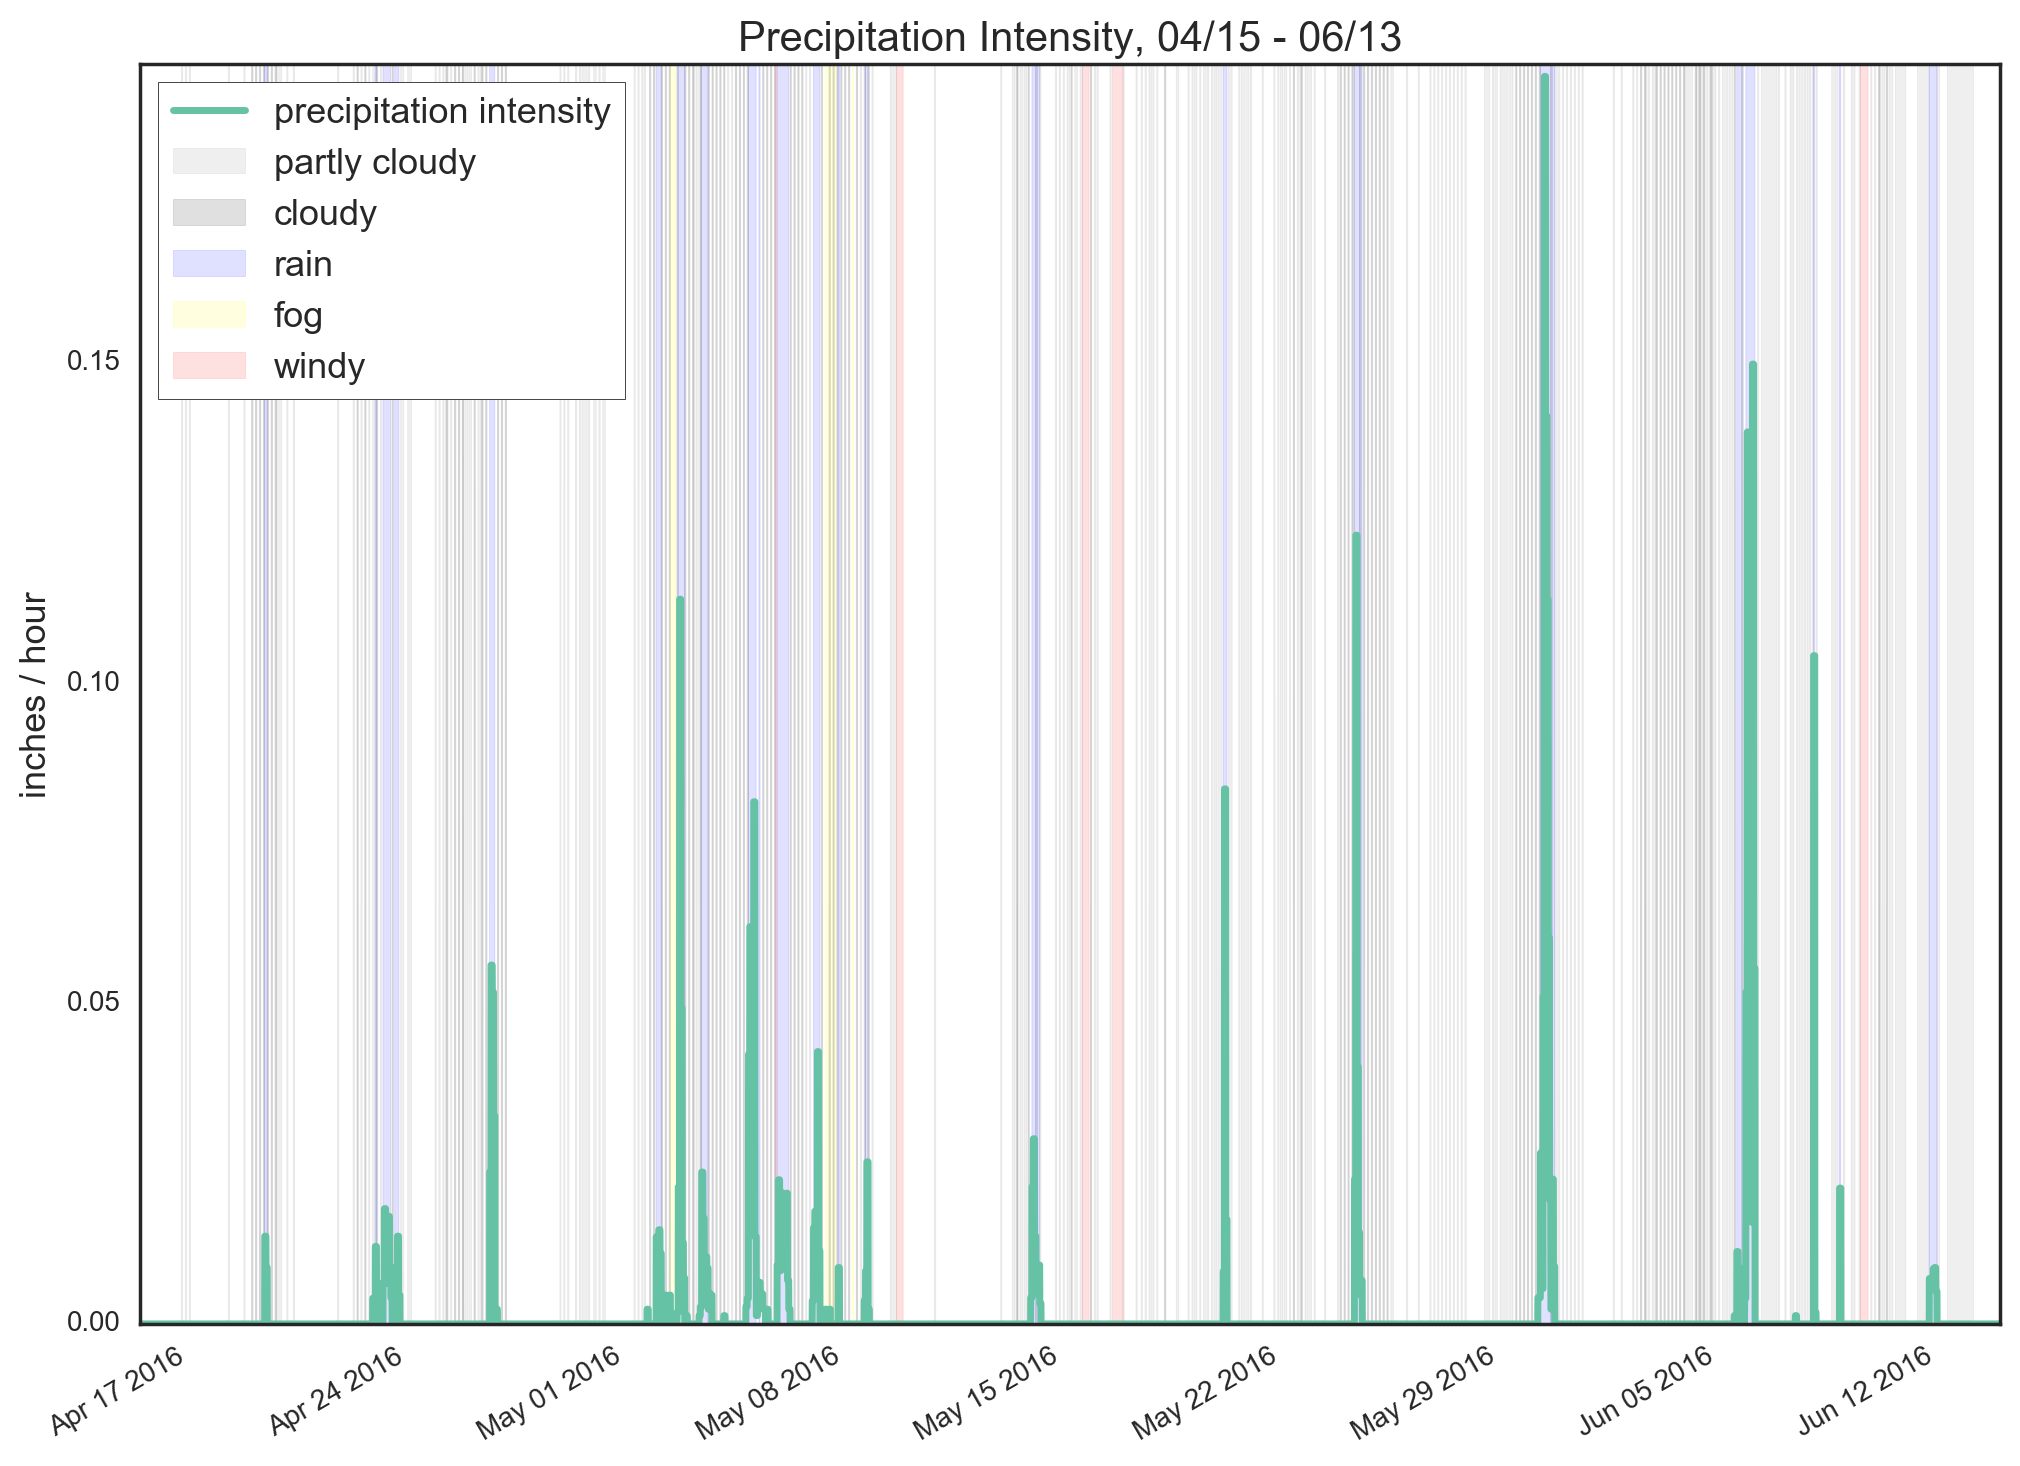
\includegraphics[width=\textwidth]{figs/precip_intensity}               
 	 \caption{Precipitation Intensity during Test Period}
  	\label{fig:precip_intensity}
\end{figure}

\begin{figure}[htb]
 	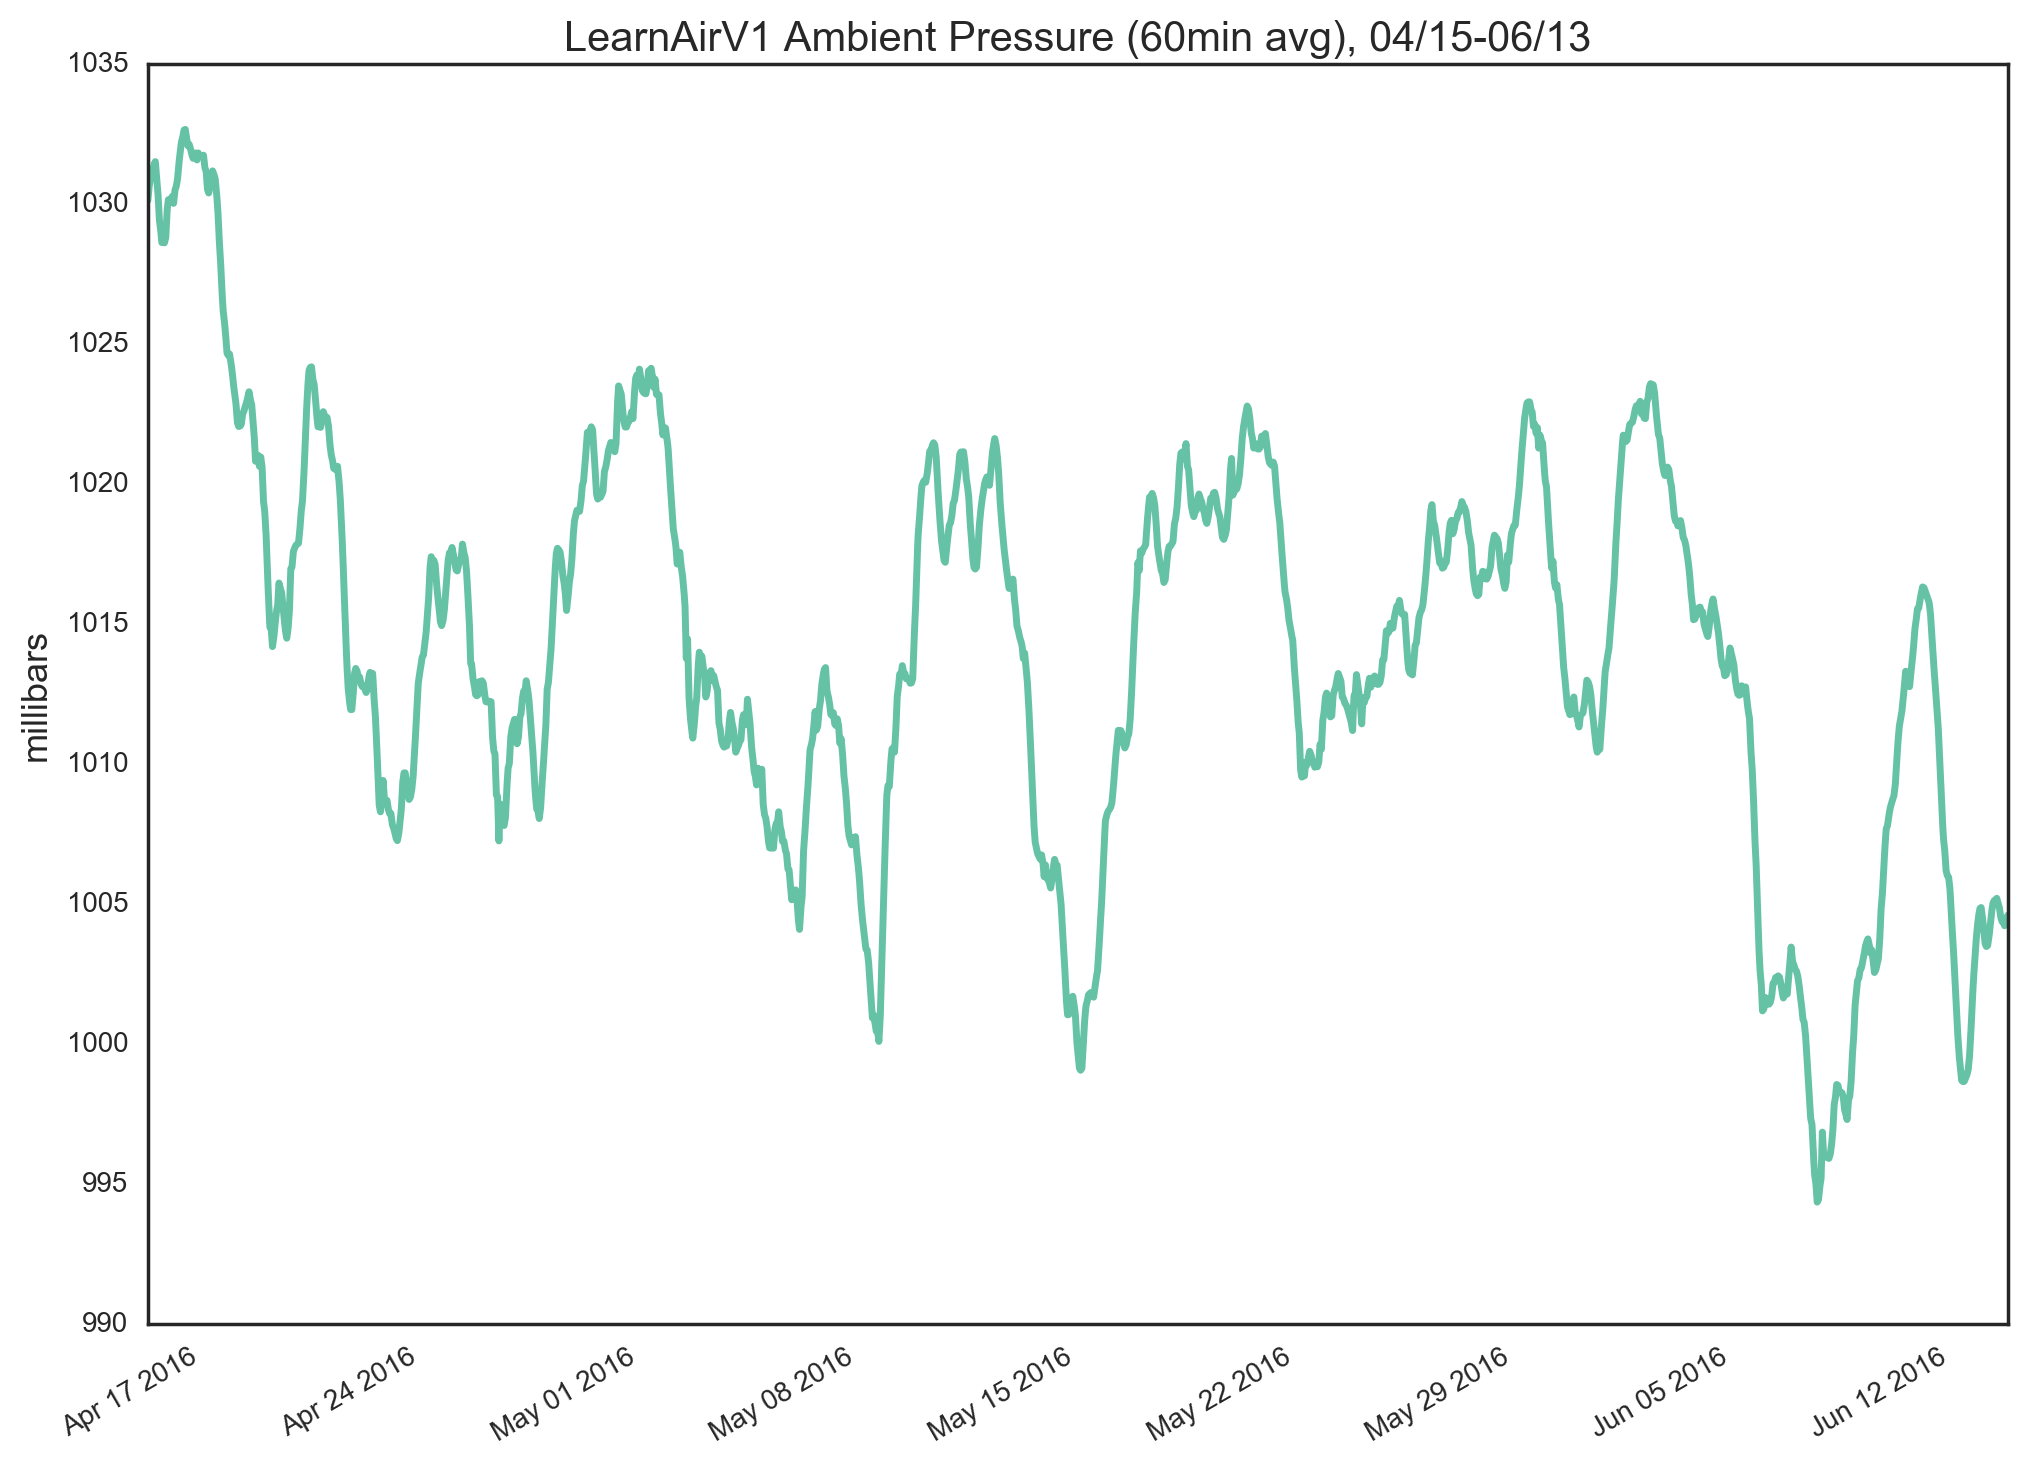
\includegraphics[width=\textwidth]{figs/ambient_pressure}               
 	 \caption{Ambient Pressure during Test Period}
  	\label{fig:ambient_pressure}
\end{figure}

\begin{figure}[htb]
 	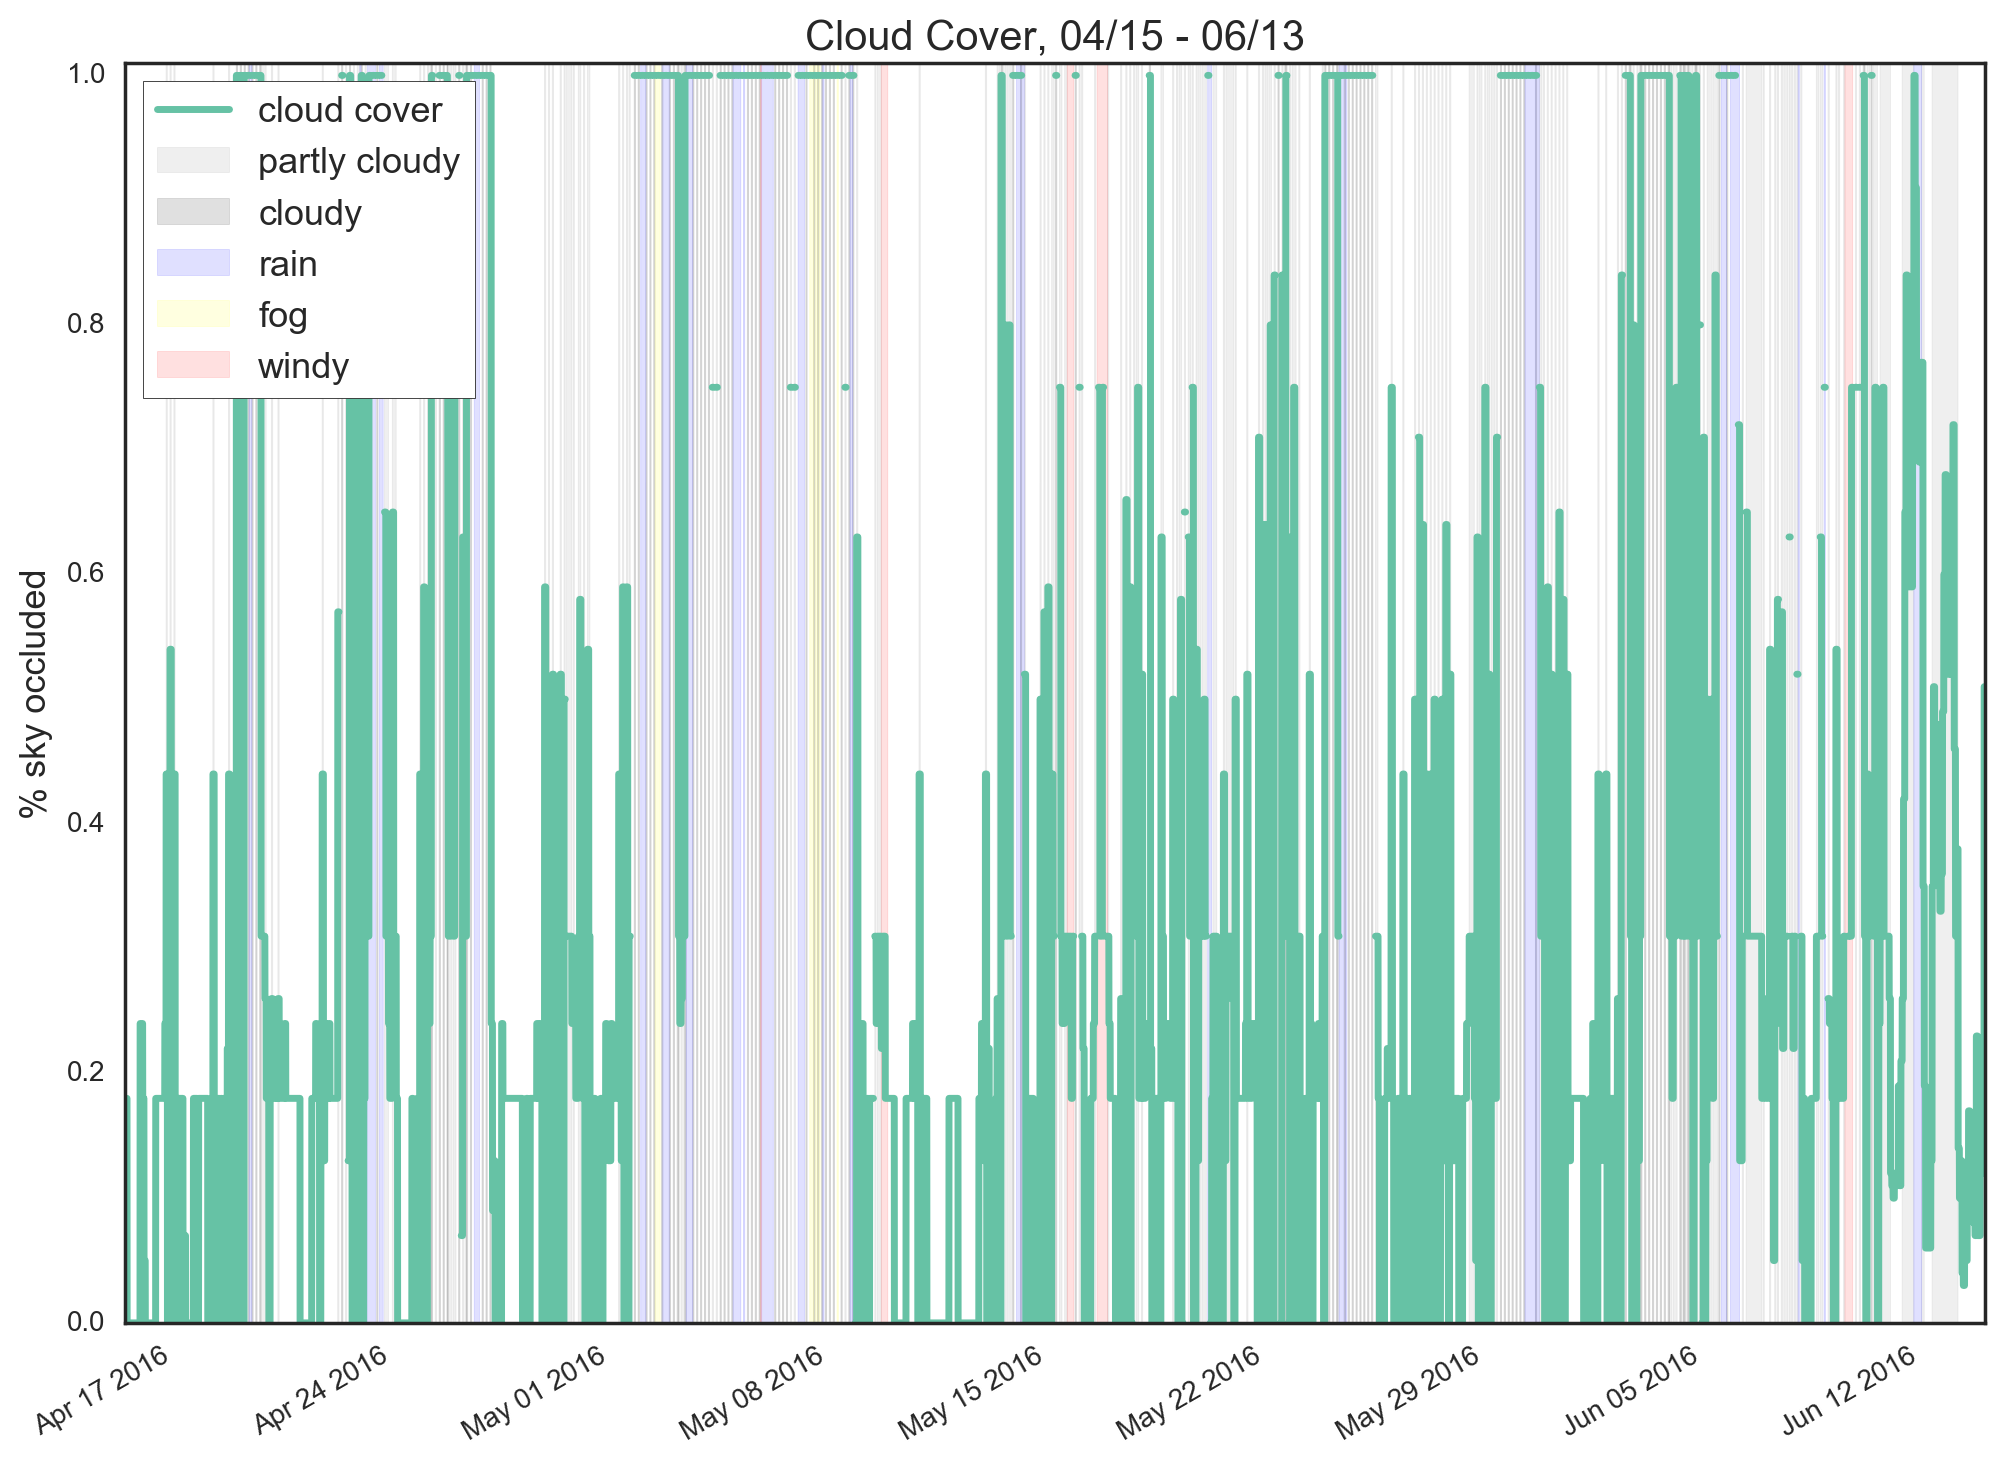
\includegraphics[width=\textwidth]{figs/cloud_cover}               
 	 \caption{Cloud Cover during Test Period}
  	\label{fig:cloud_cover}
\end{figure}

\begin{figure}[htb]
 	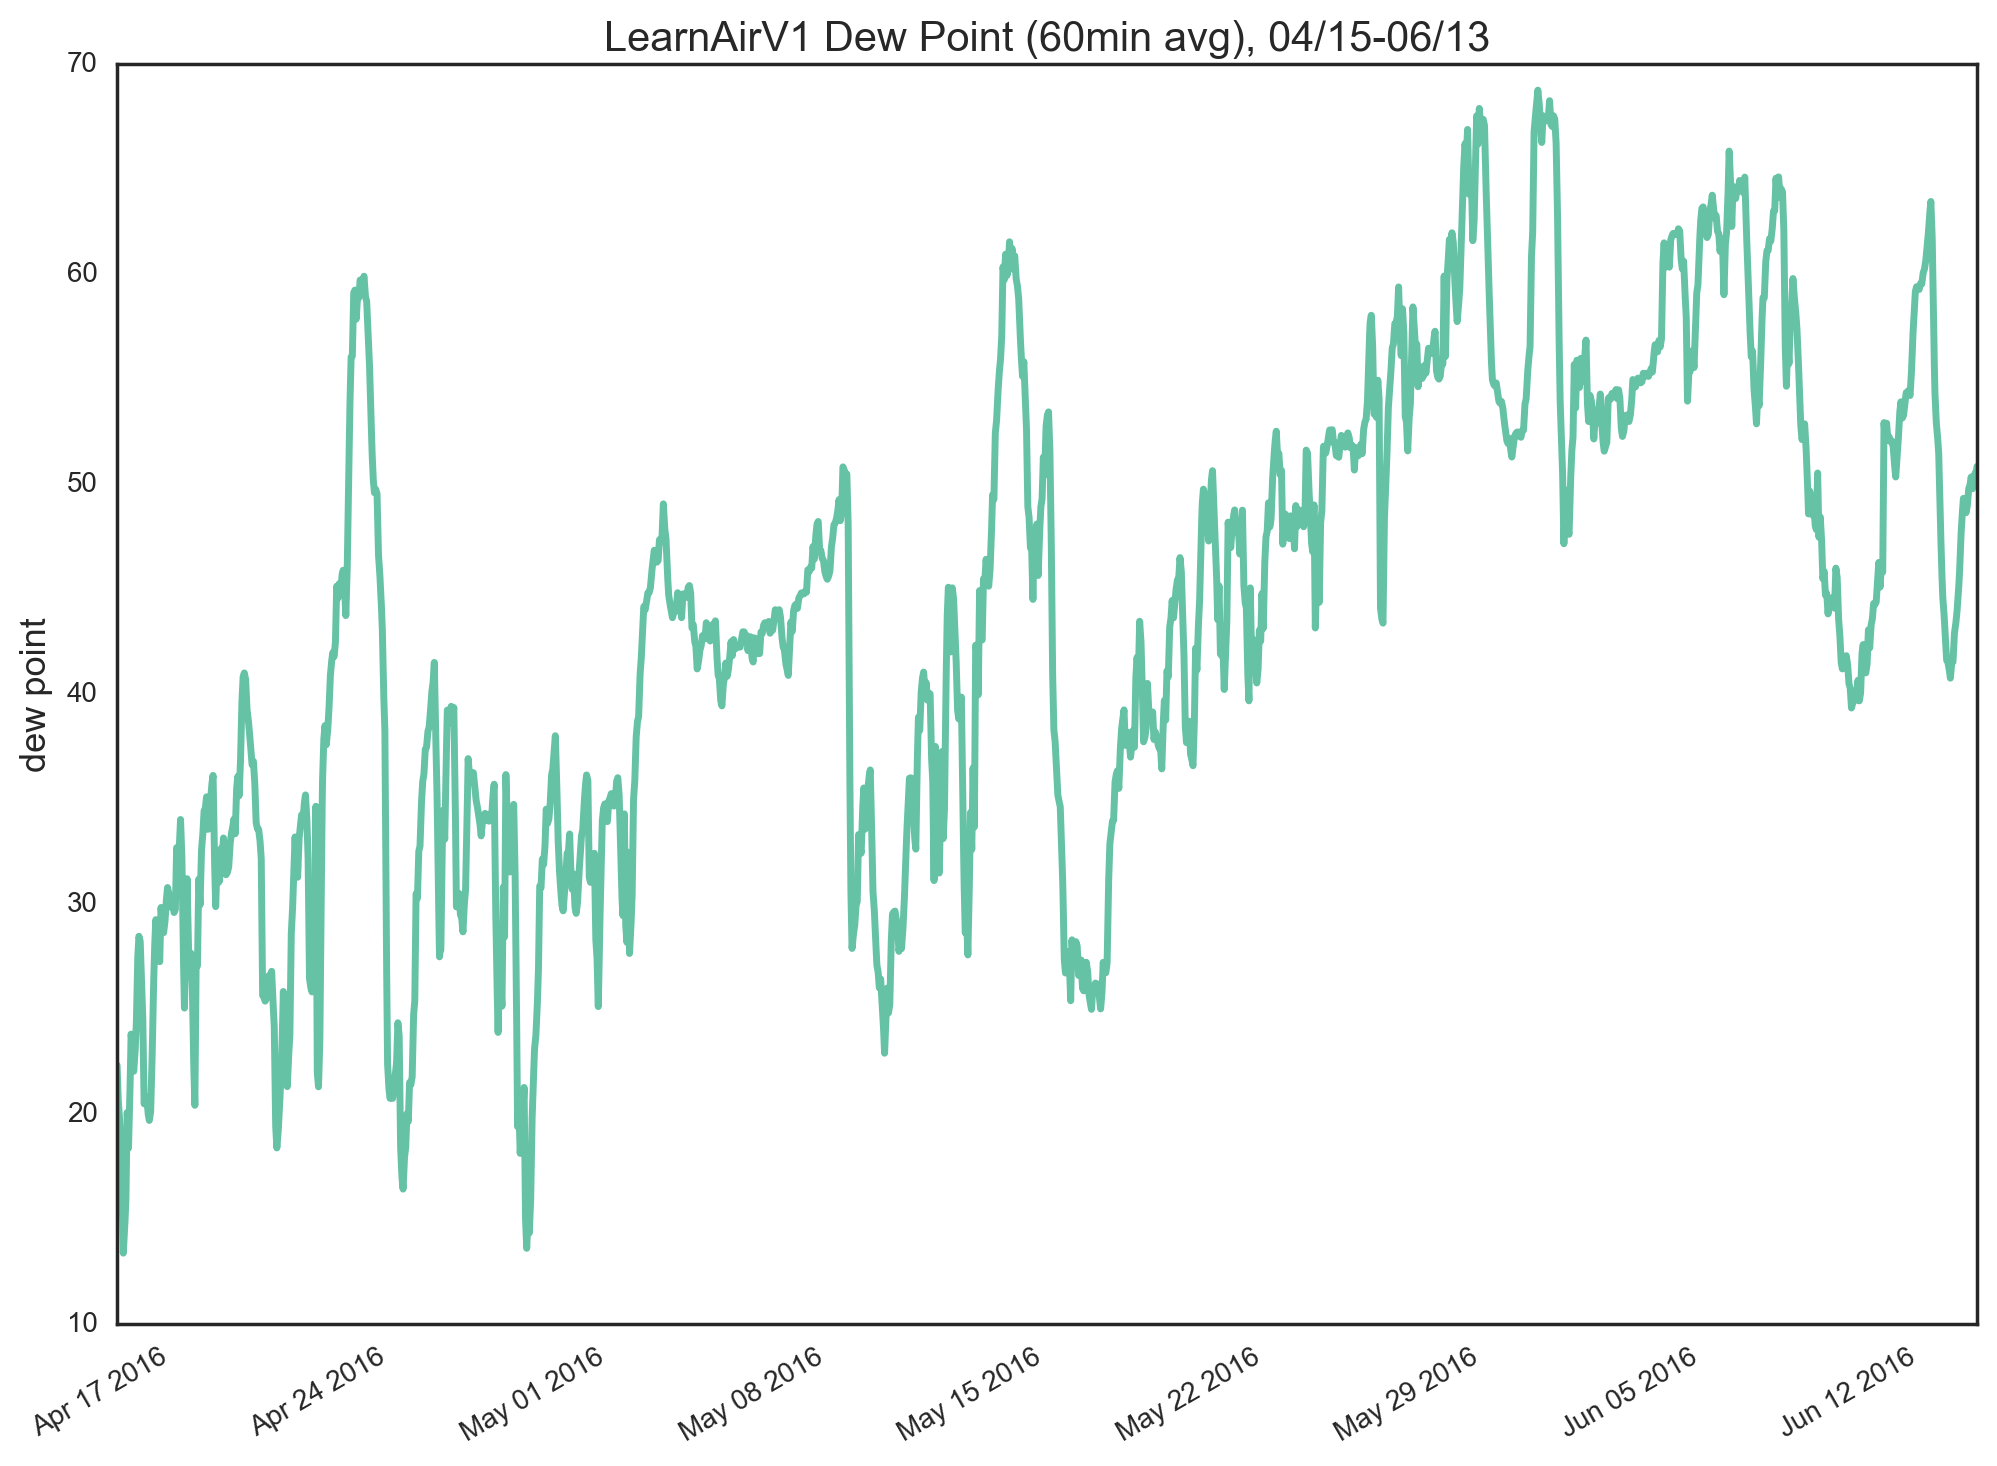
\includegraphics[width=\textwidth]{figs/dew}               
 	 \caption{Dew during Test Period}
  	\label{fig:dew}
\end{figure}

\begin{figure}[htb]
 	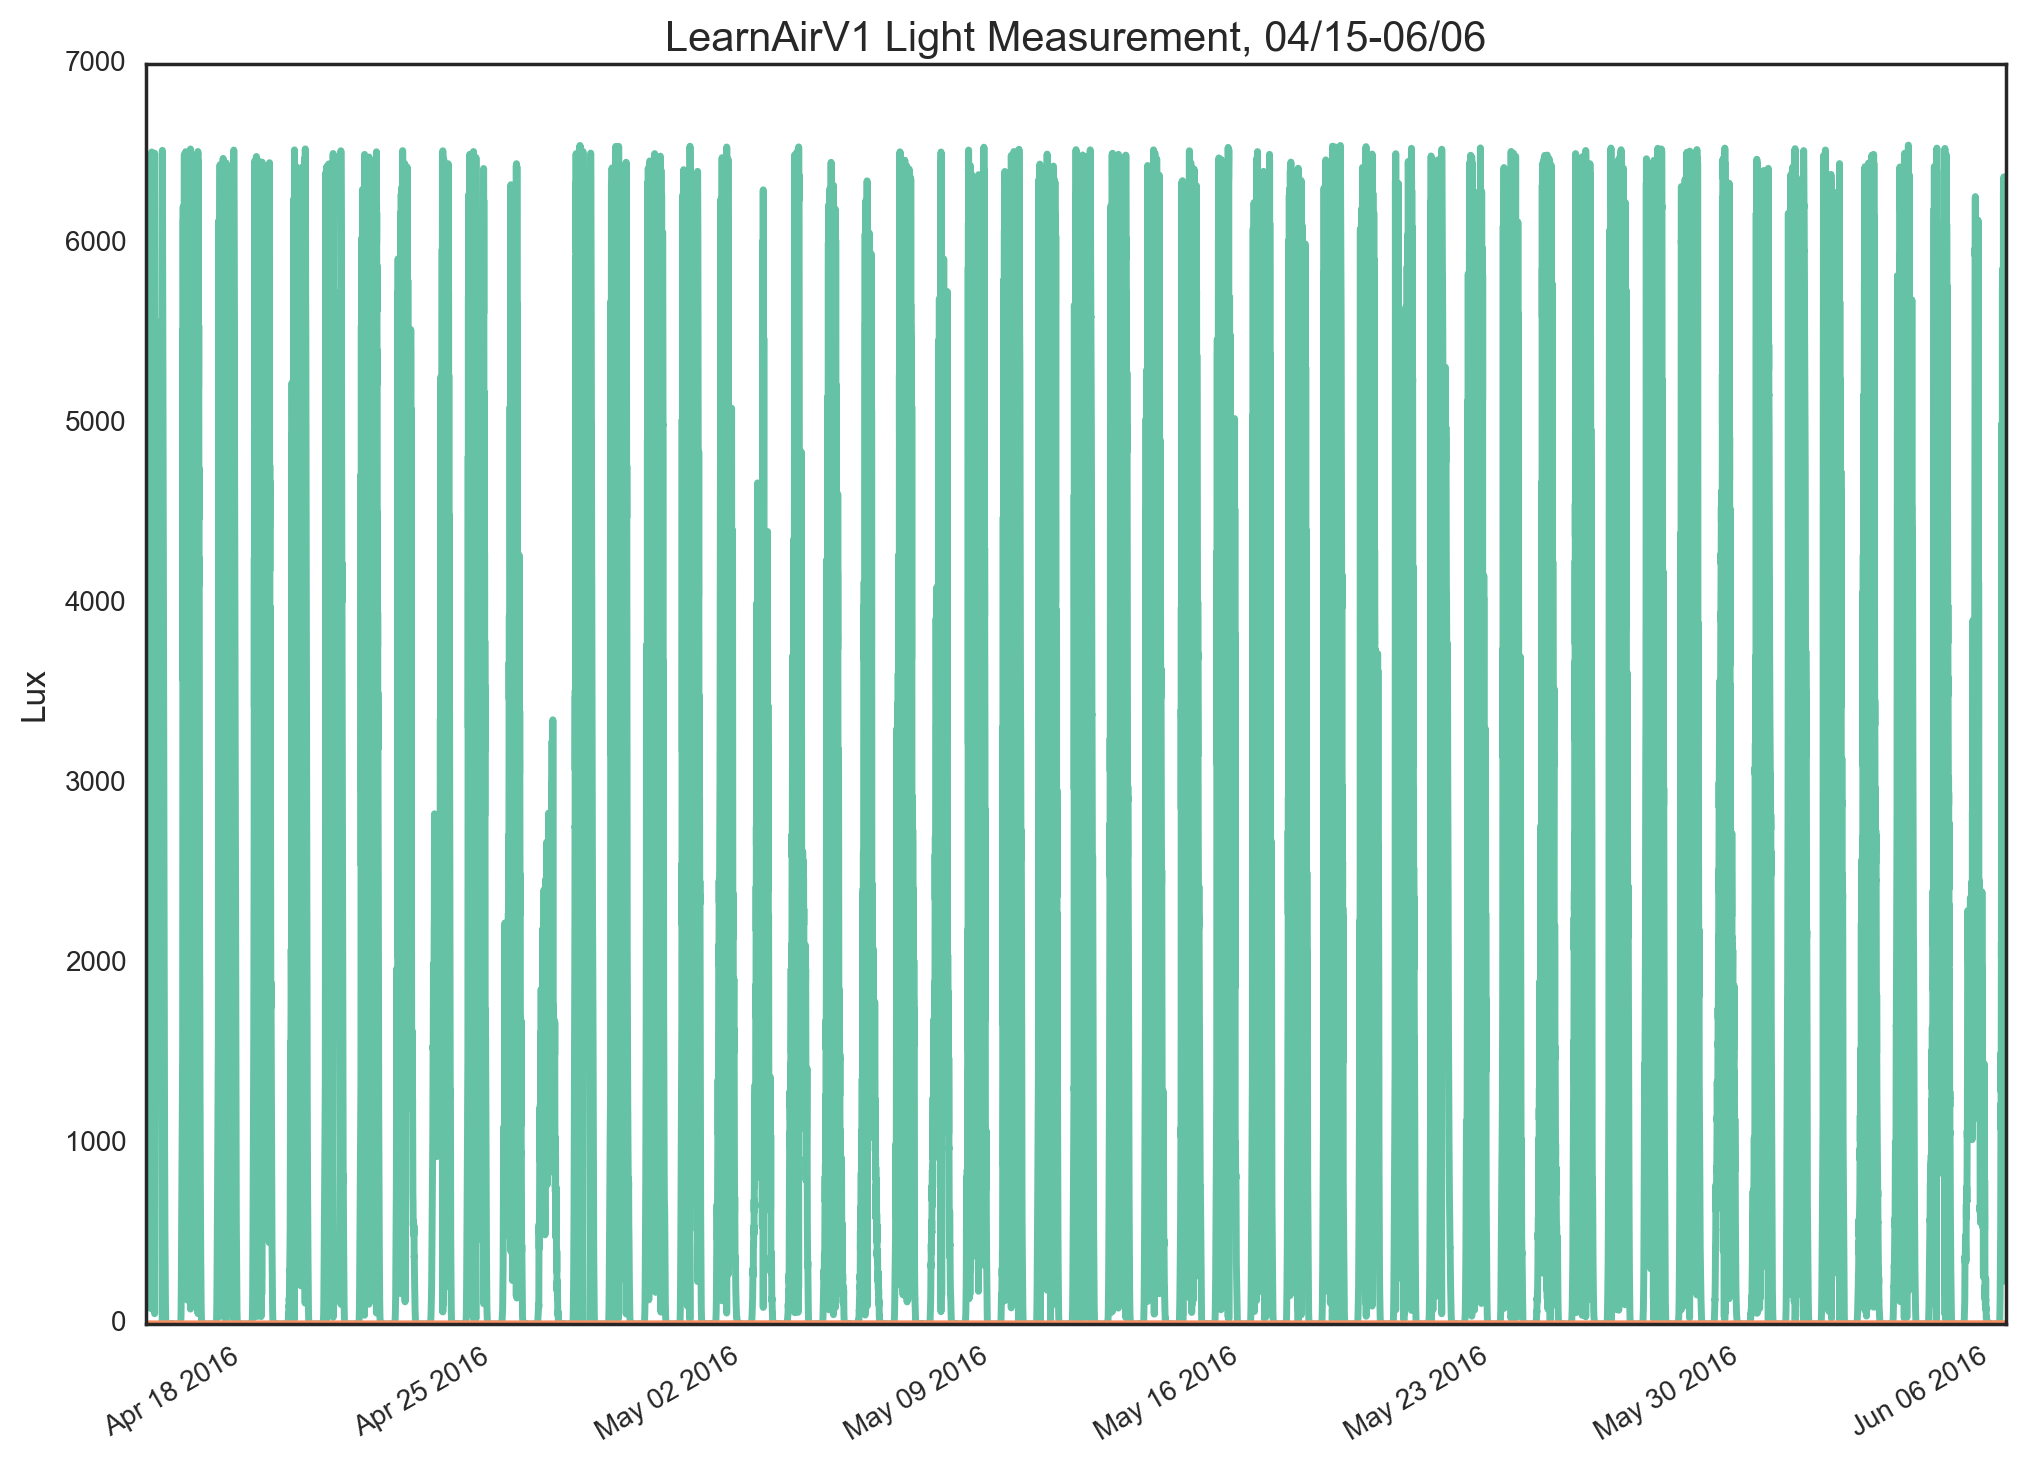
\includegraphics[width=\textwidth]{figs/lux}               
 	 \caption{Lux during Test Period}
  	\label{fig:lux}
\end{figure}

\begin{figure}[htb]
 	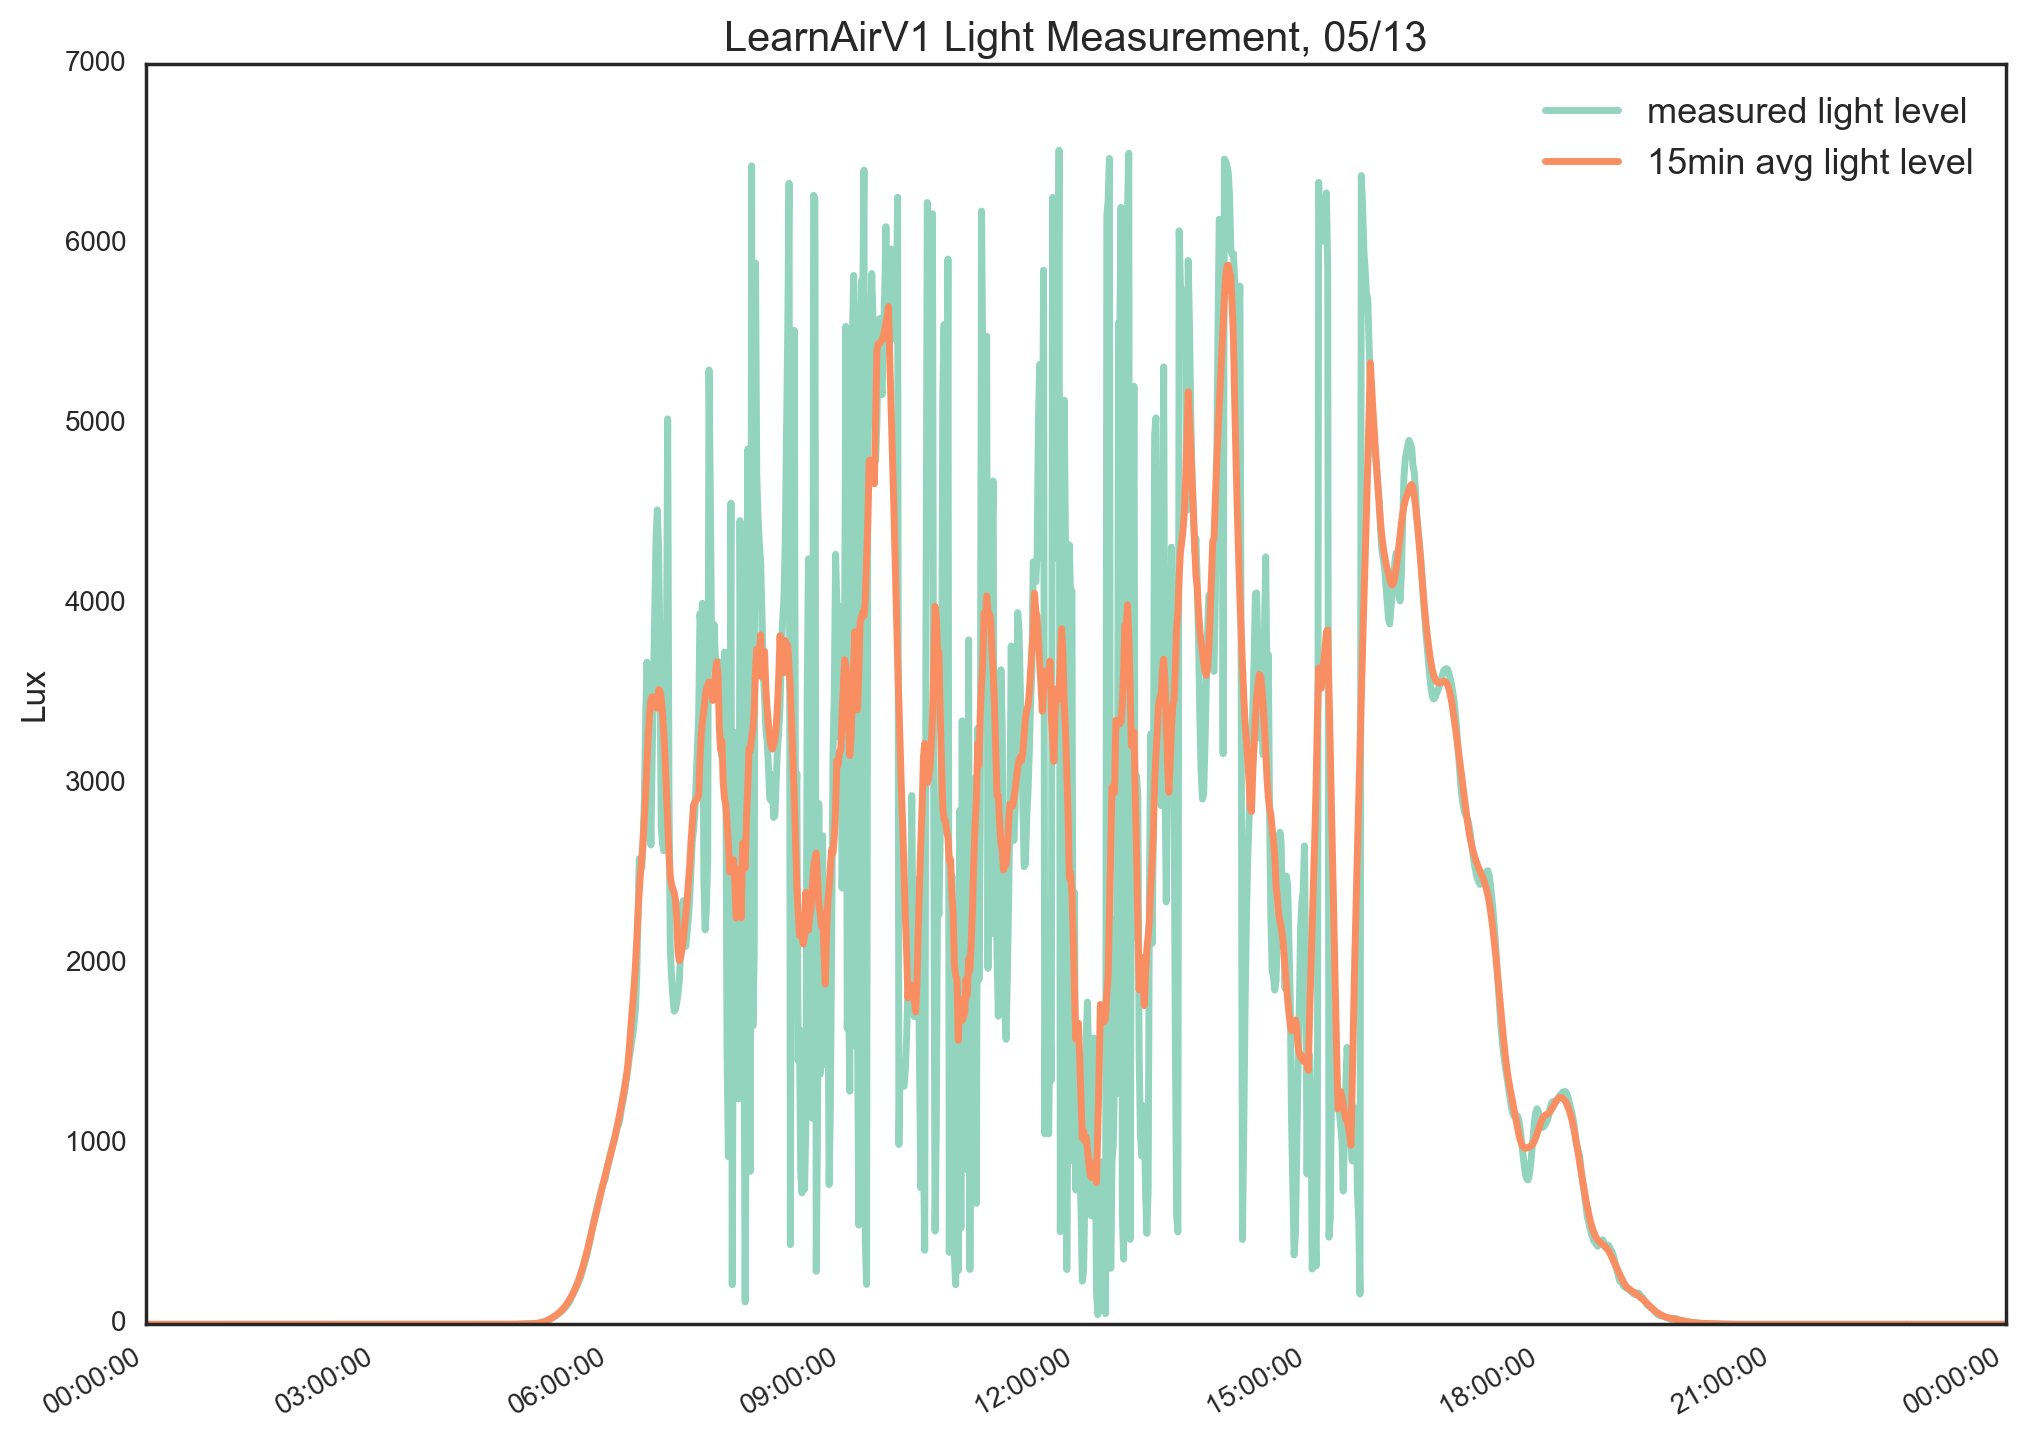
\includegraphics[width=\textwidth]{figs/lux_zoomed}               
 	 \caption{Lux during Test Period}
  	\label{fig:lux_zoomed}
\end{figure}

\clearpage

\FloatBarrier

\enlargethispage{2.5cm}

\begin{figure}[!b]
 	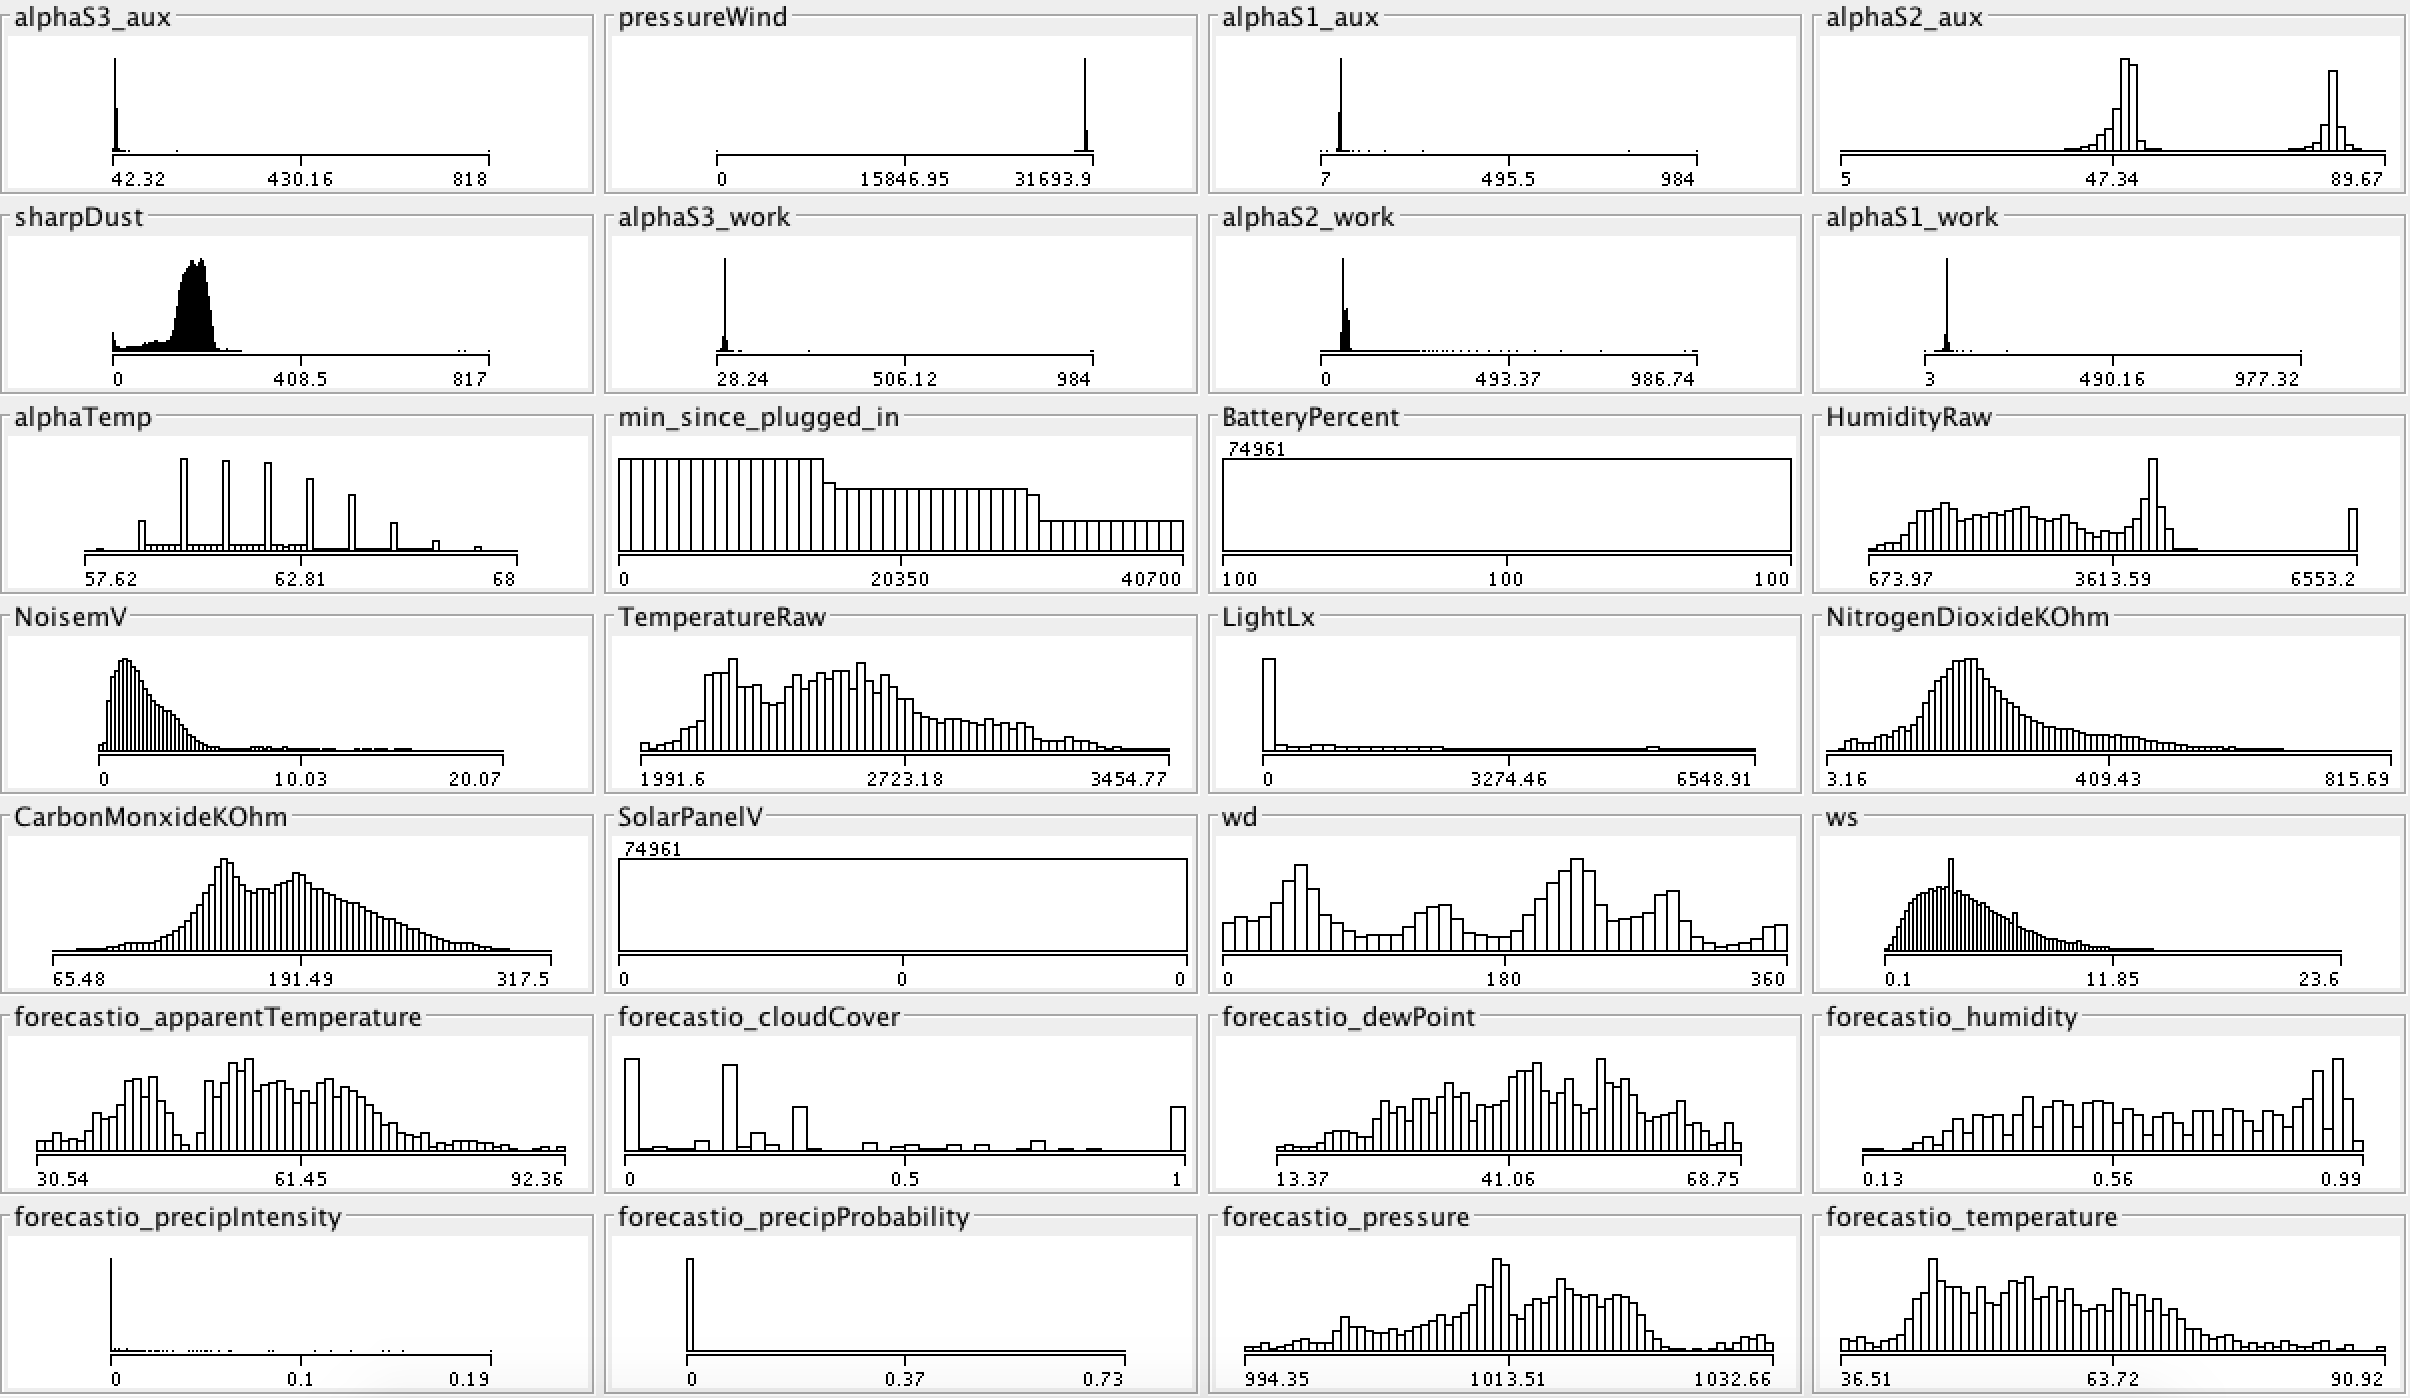
\includegraphics[width=\textwidth-4cc]{weka/features1}  
	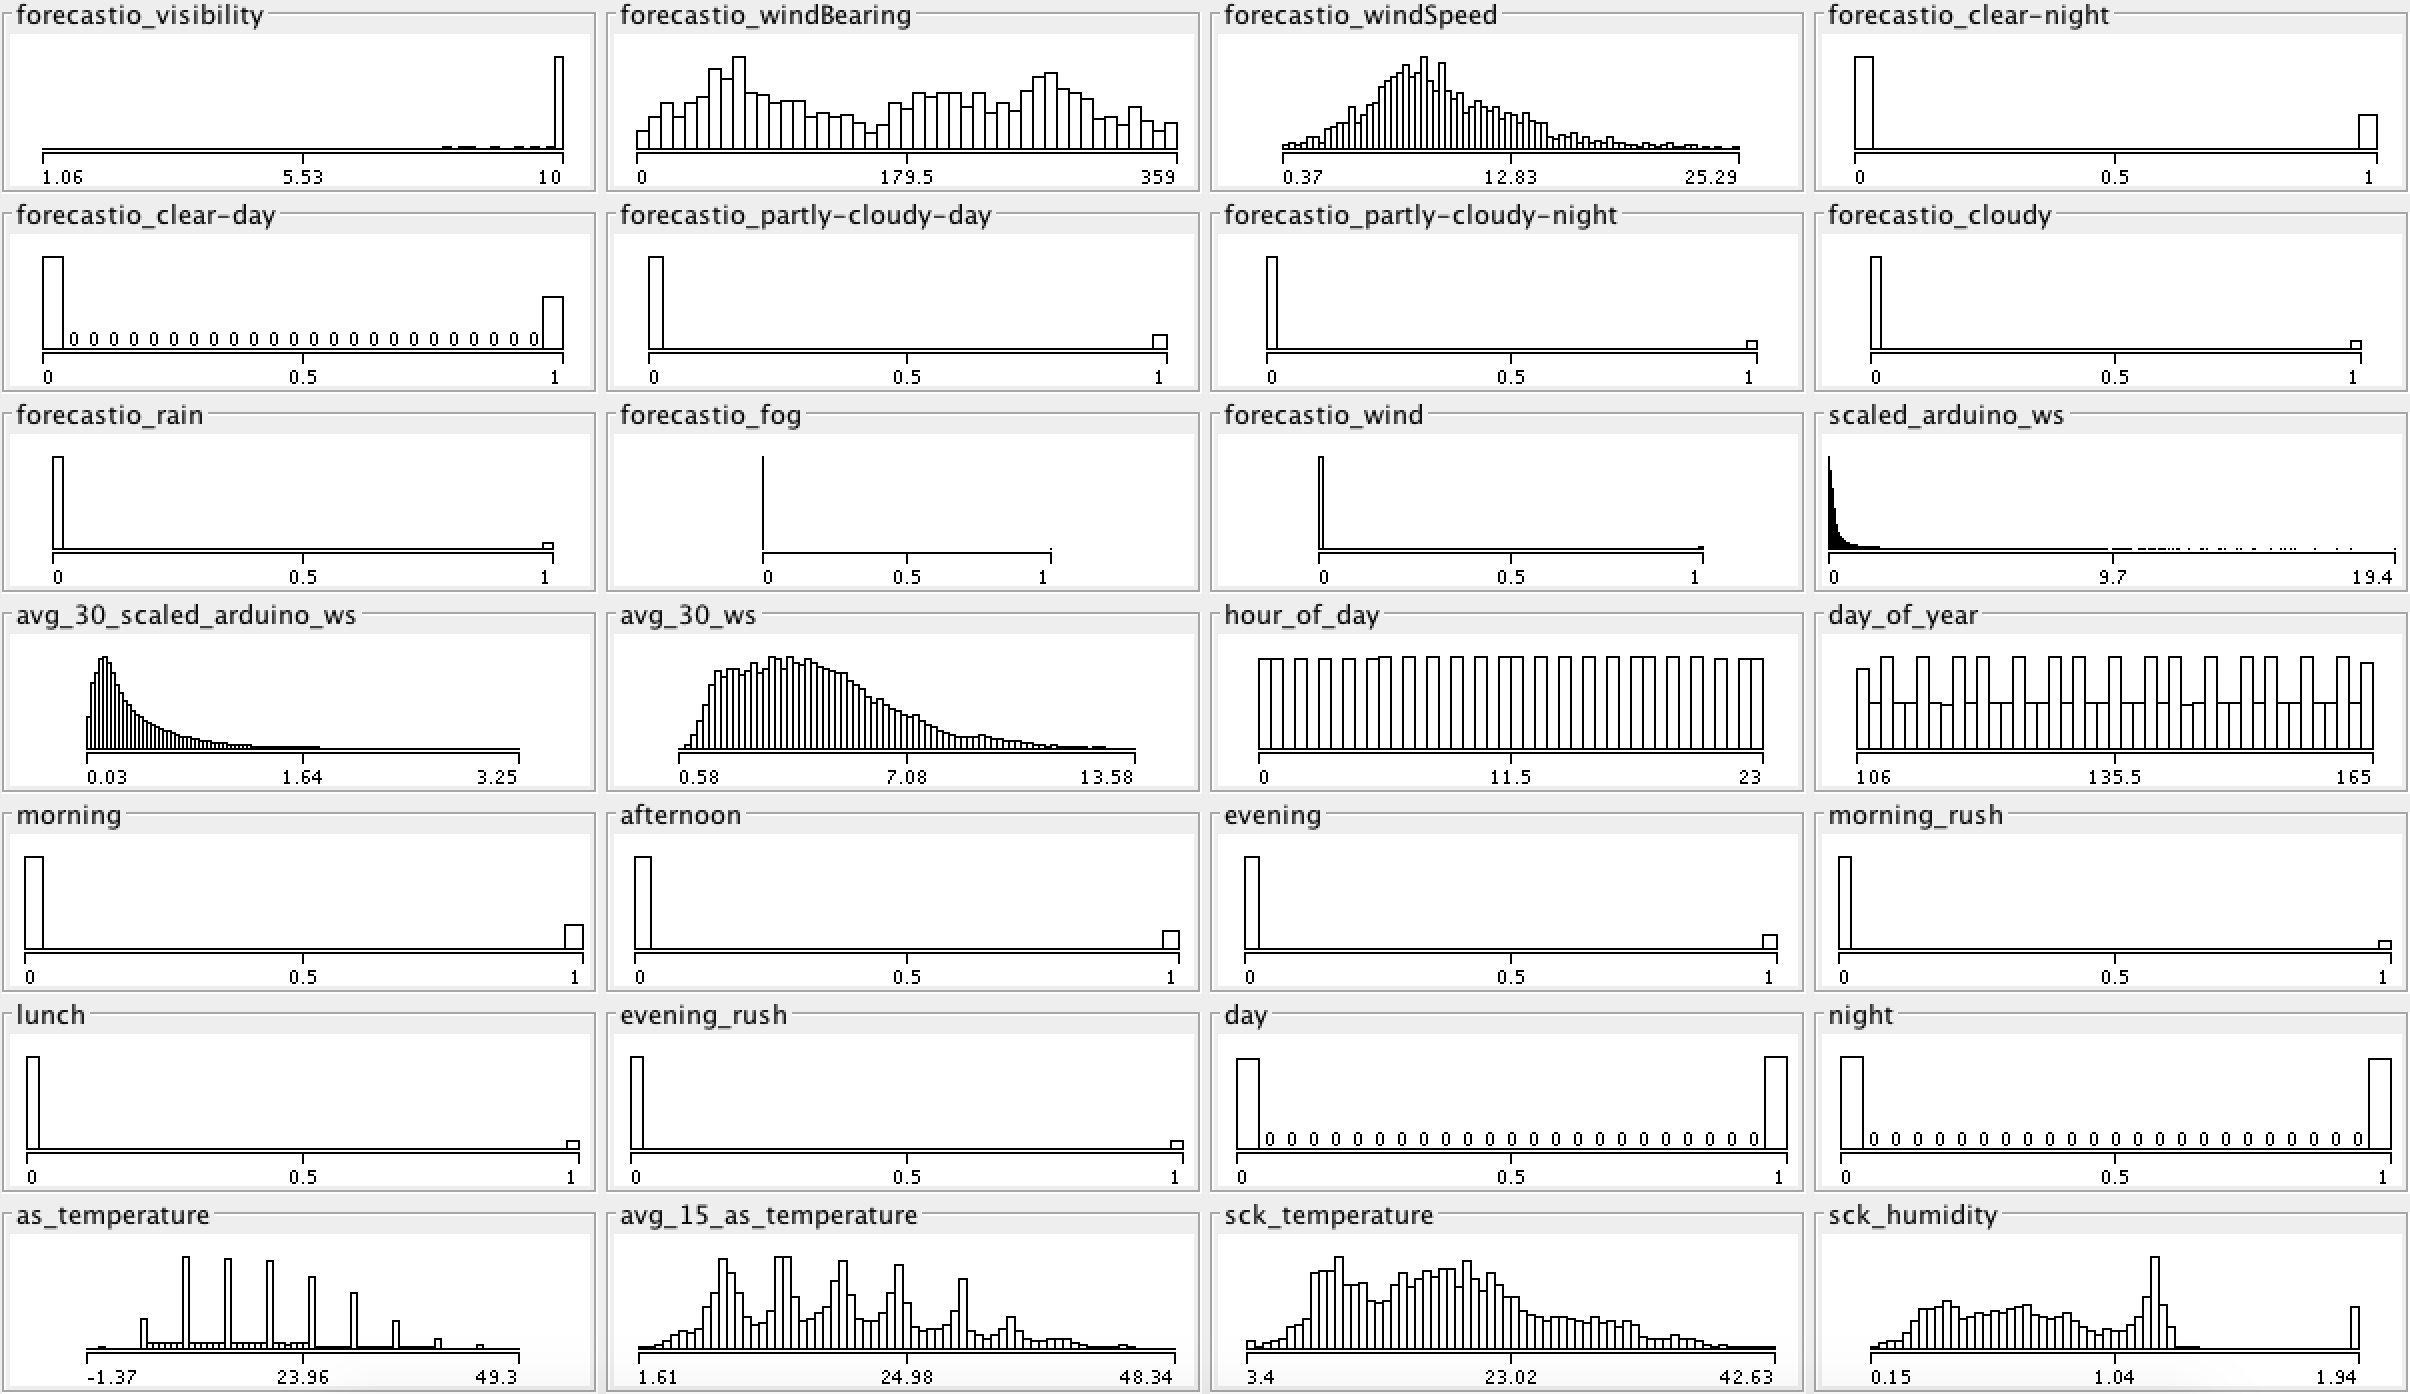
\includegraphics[width=\textwidth-4cc]{weka/features2}    
	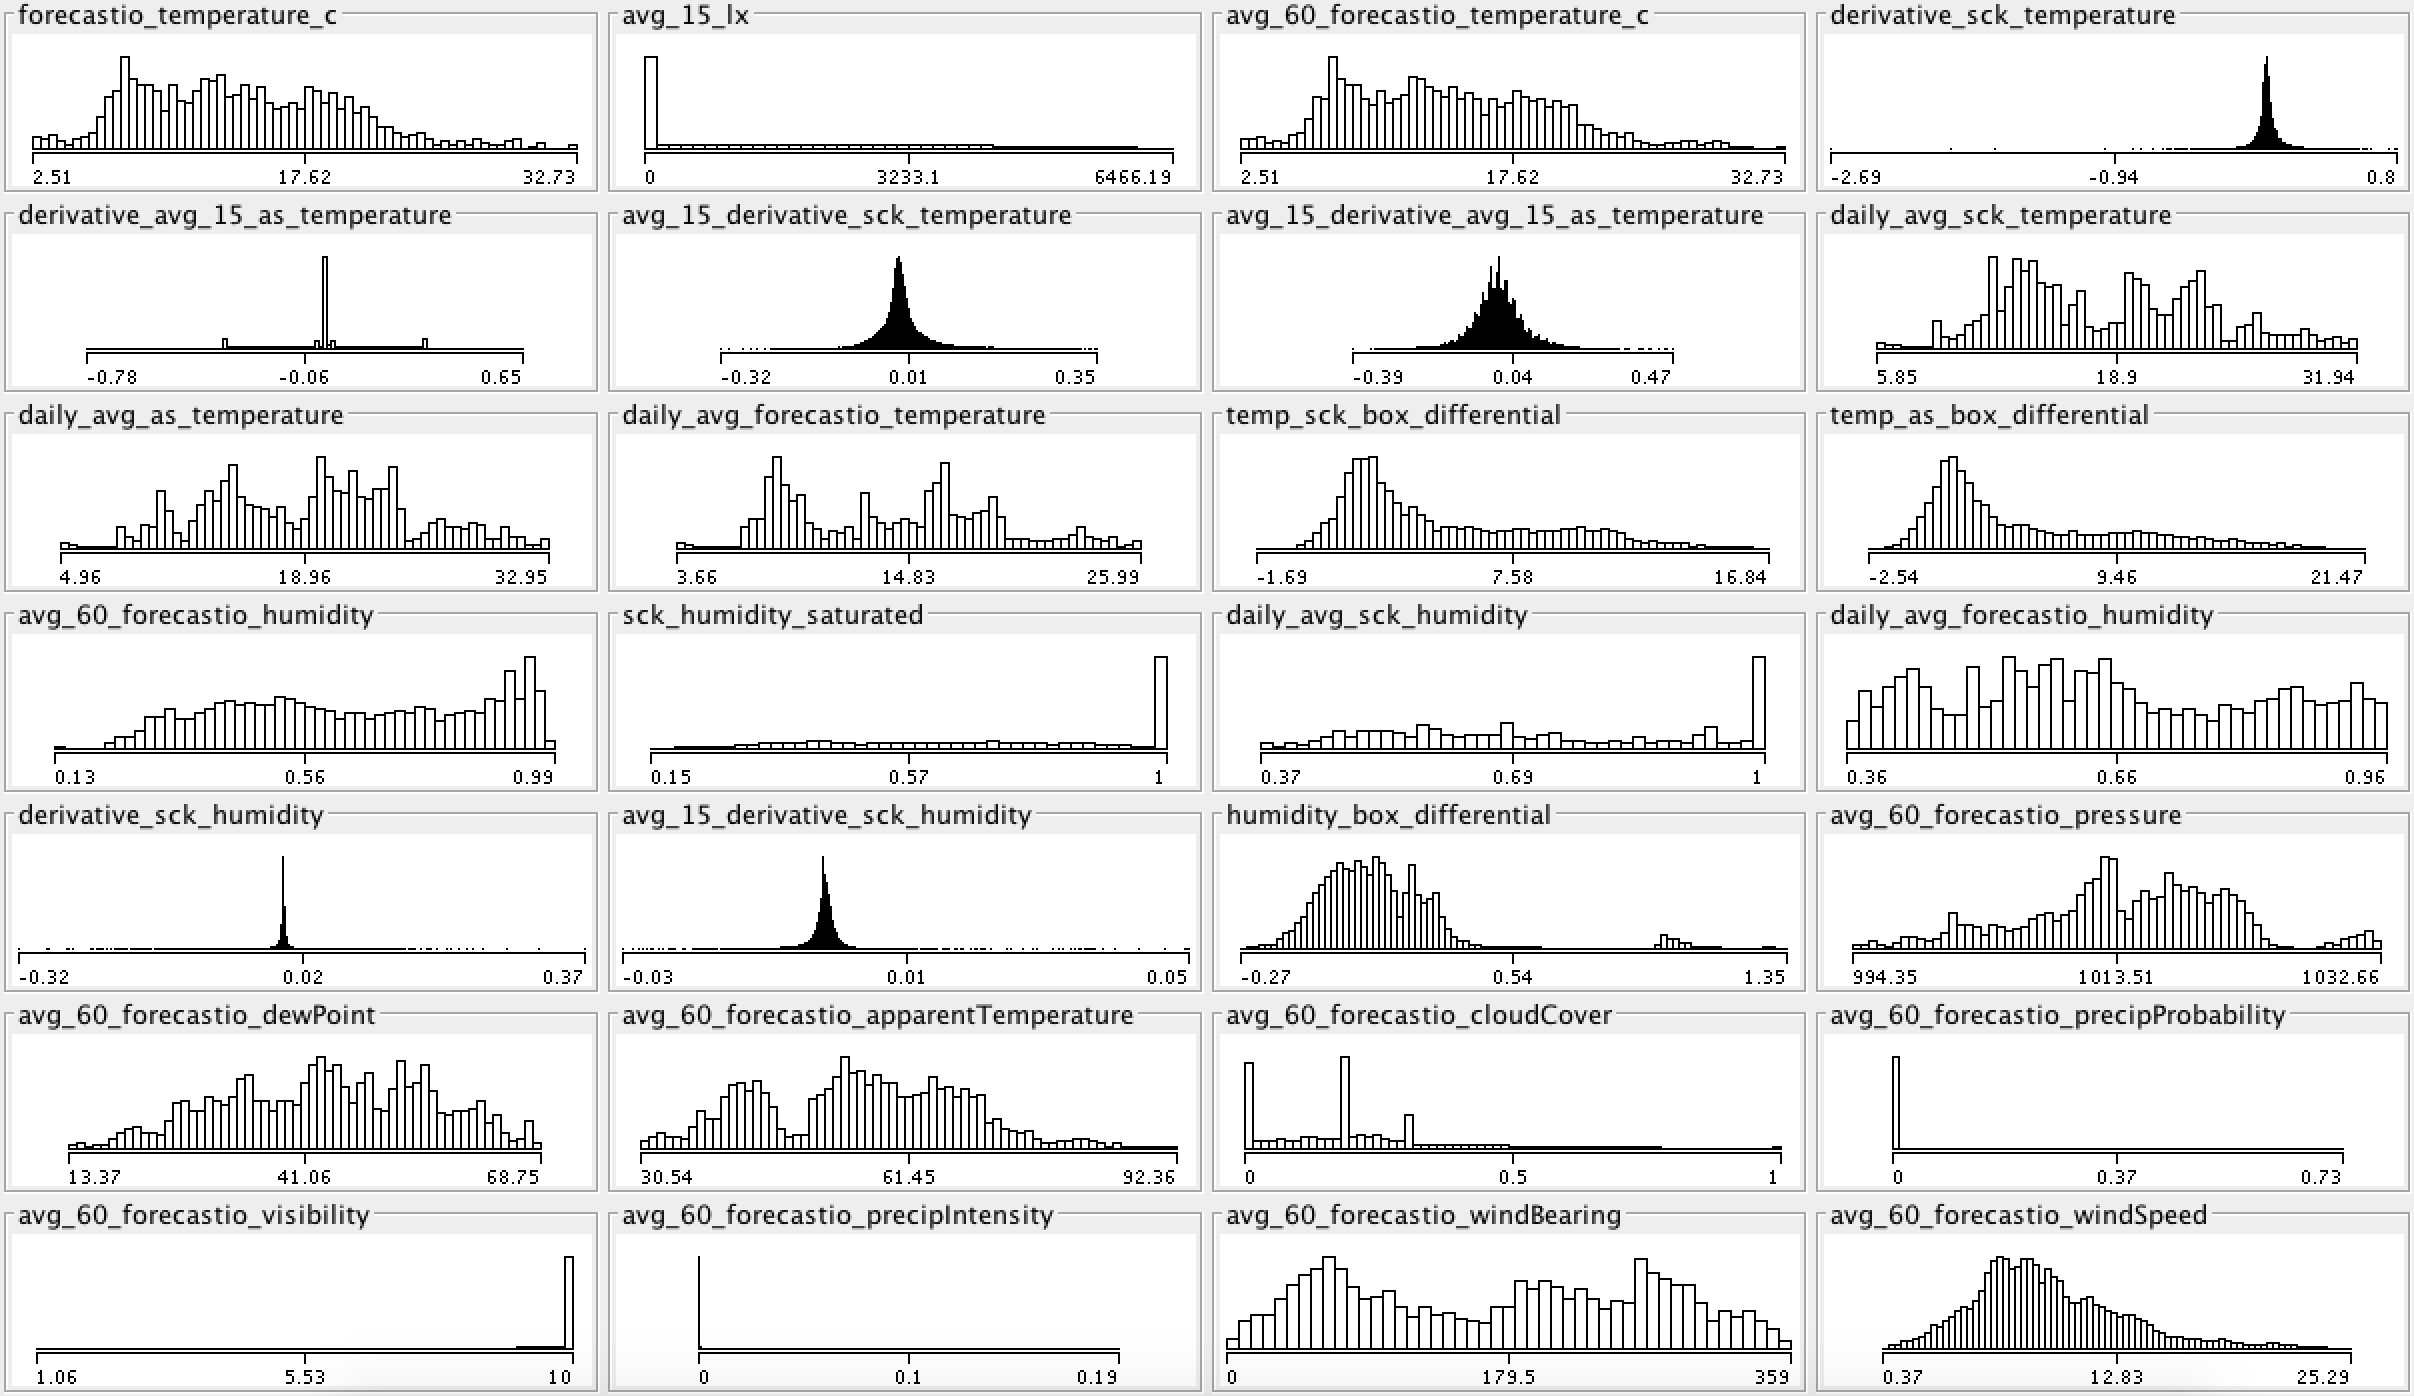
\includegraphics[width=\textwidth-4cc]{weka/features3}  
	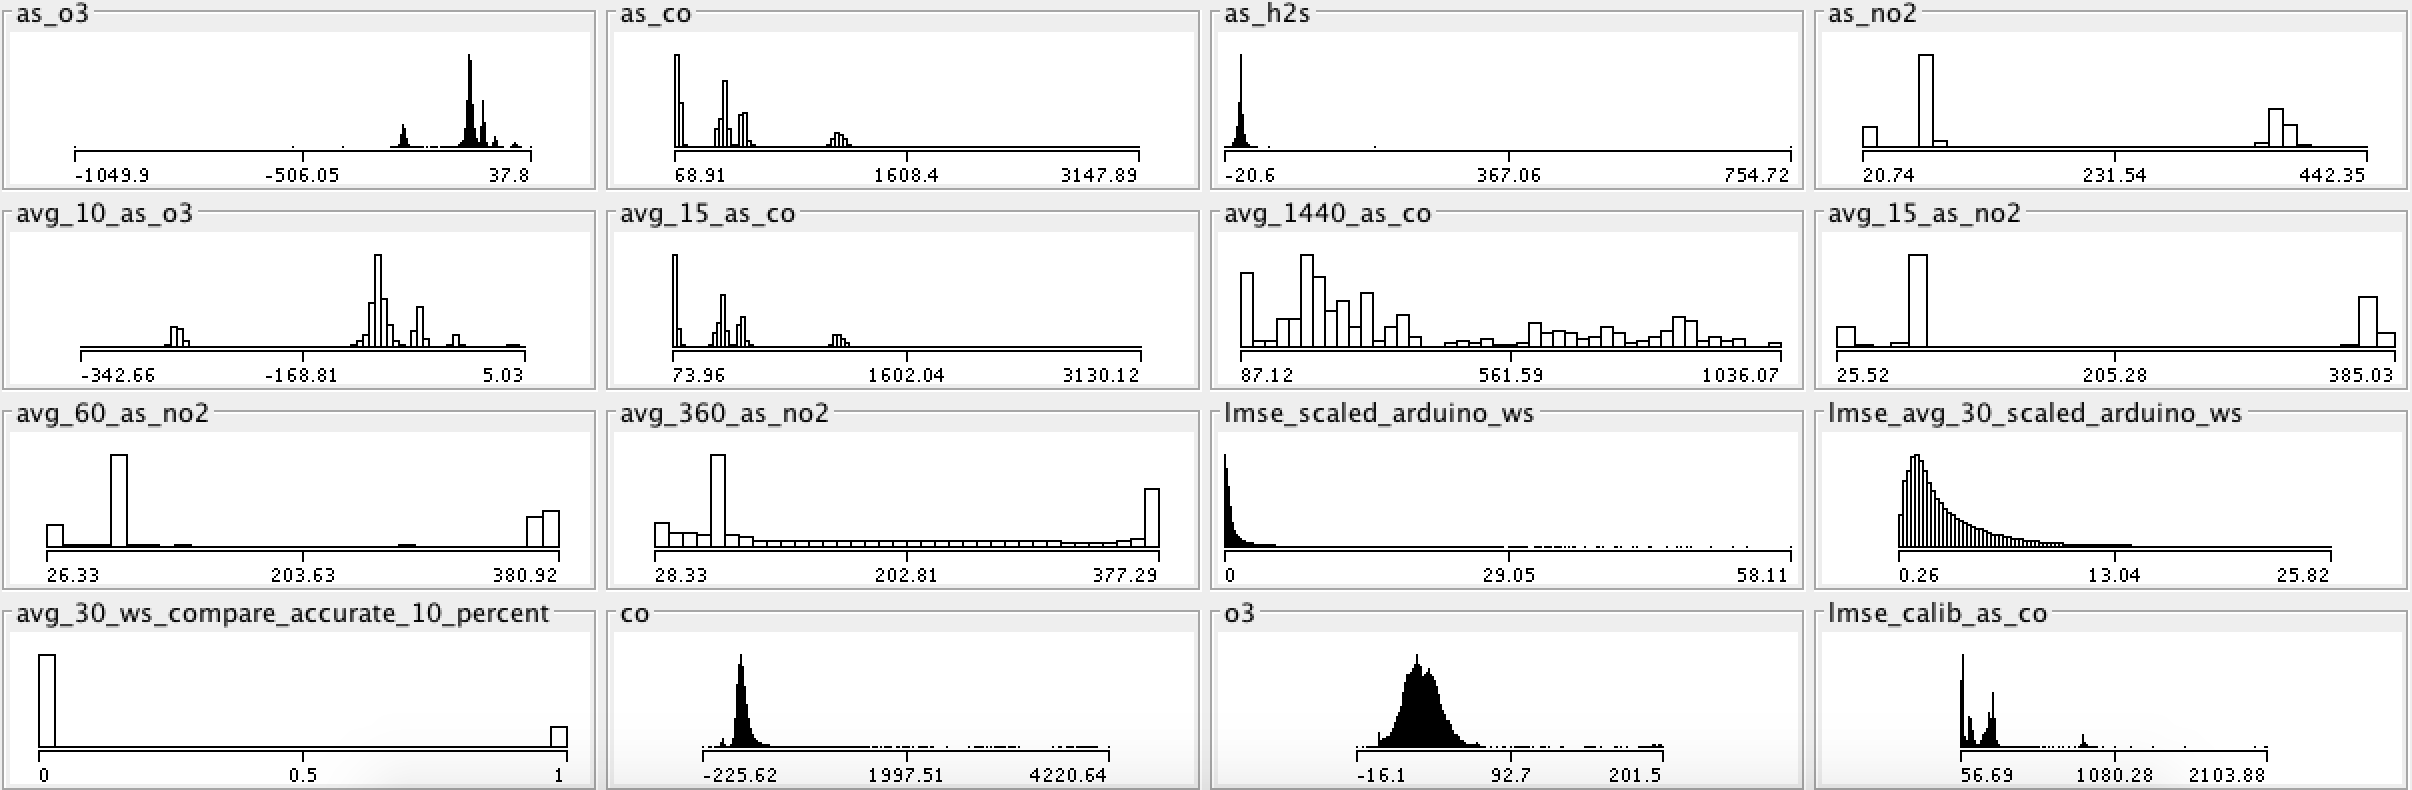
\includegraphics[width=\textwidth-4cc]{weka/features4}                  
         \caption{ML feature histograms plotted with WEKA Tool}
 	 \label{fig:weka_features}
\end{figure}



\section{Data Pre-Processing}

\section{Features}


The figure below includes most of the machine learning feature distributions plotted using Weka.

\FloatBarrier
\section{SmartCitizen CO}
\FloatBarrier

Following are additional plots from the SmartCitizen CO test outlining in more detail the LMSE calibration, the accuracy with a tighter 5\% threshold, a visualization of the prediction accuracy and confidence, and the top 15 random forest selected features.

\begin{figure}[!htb]
 	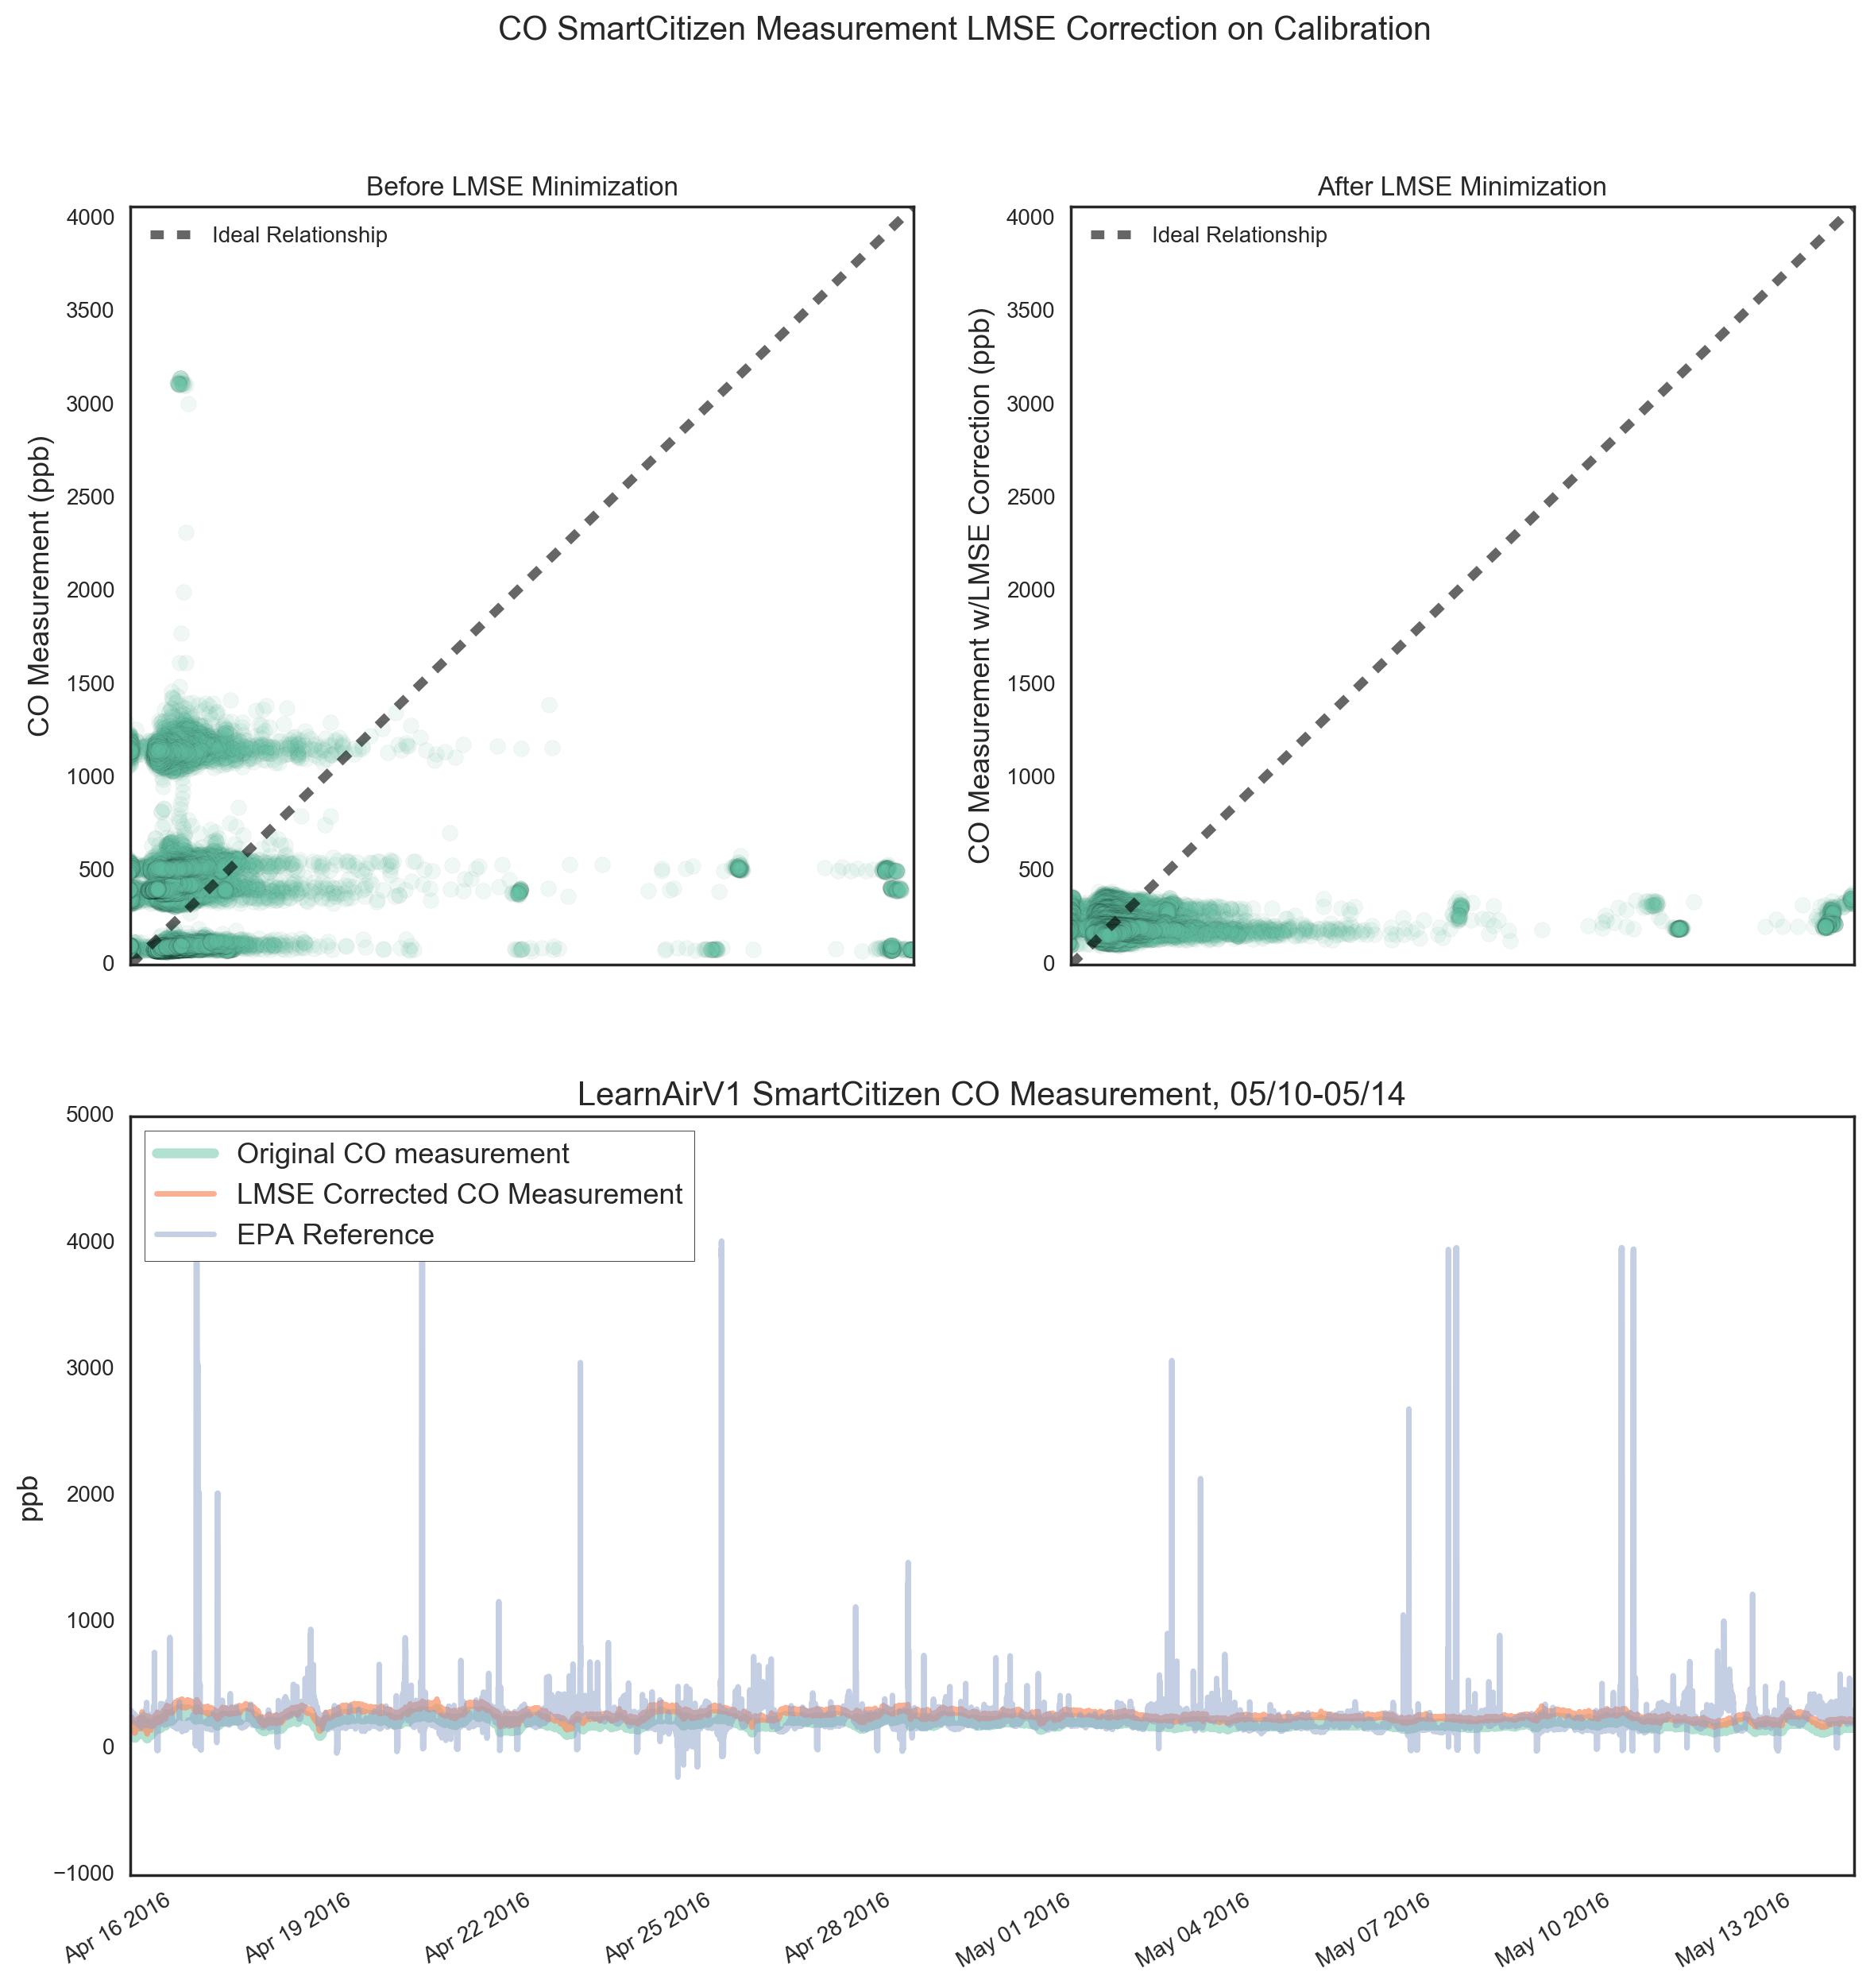
\includegraphics[width=\textwidth]{figs/sck_co_lmse}               
 	 \caption{SmartCitizen CO after LMSE Calibration}
  	\label{fig:sck_co_lmse}
\end{figure}

\begin{figure}[htb]
 	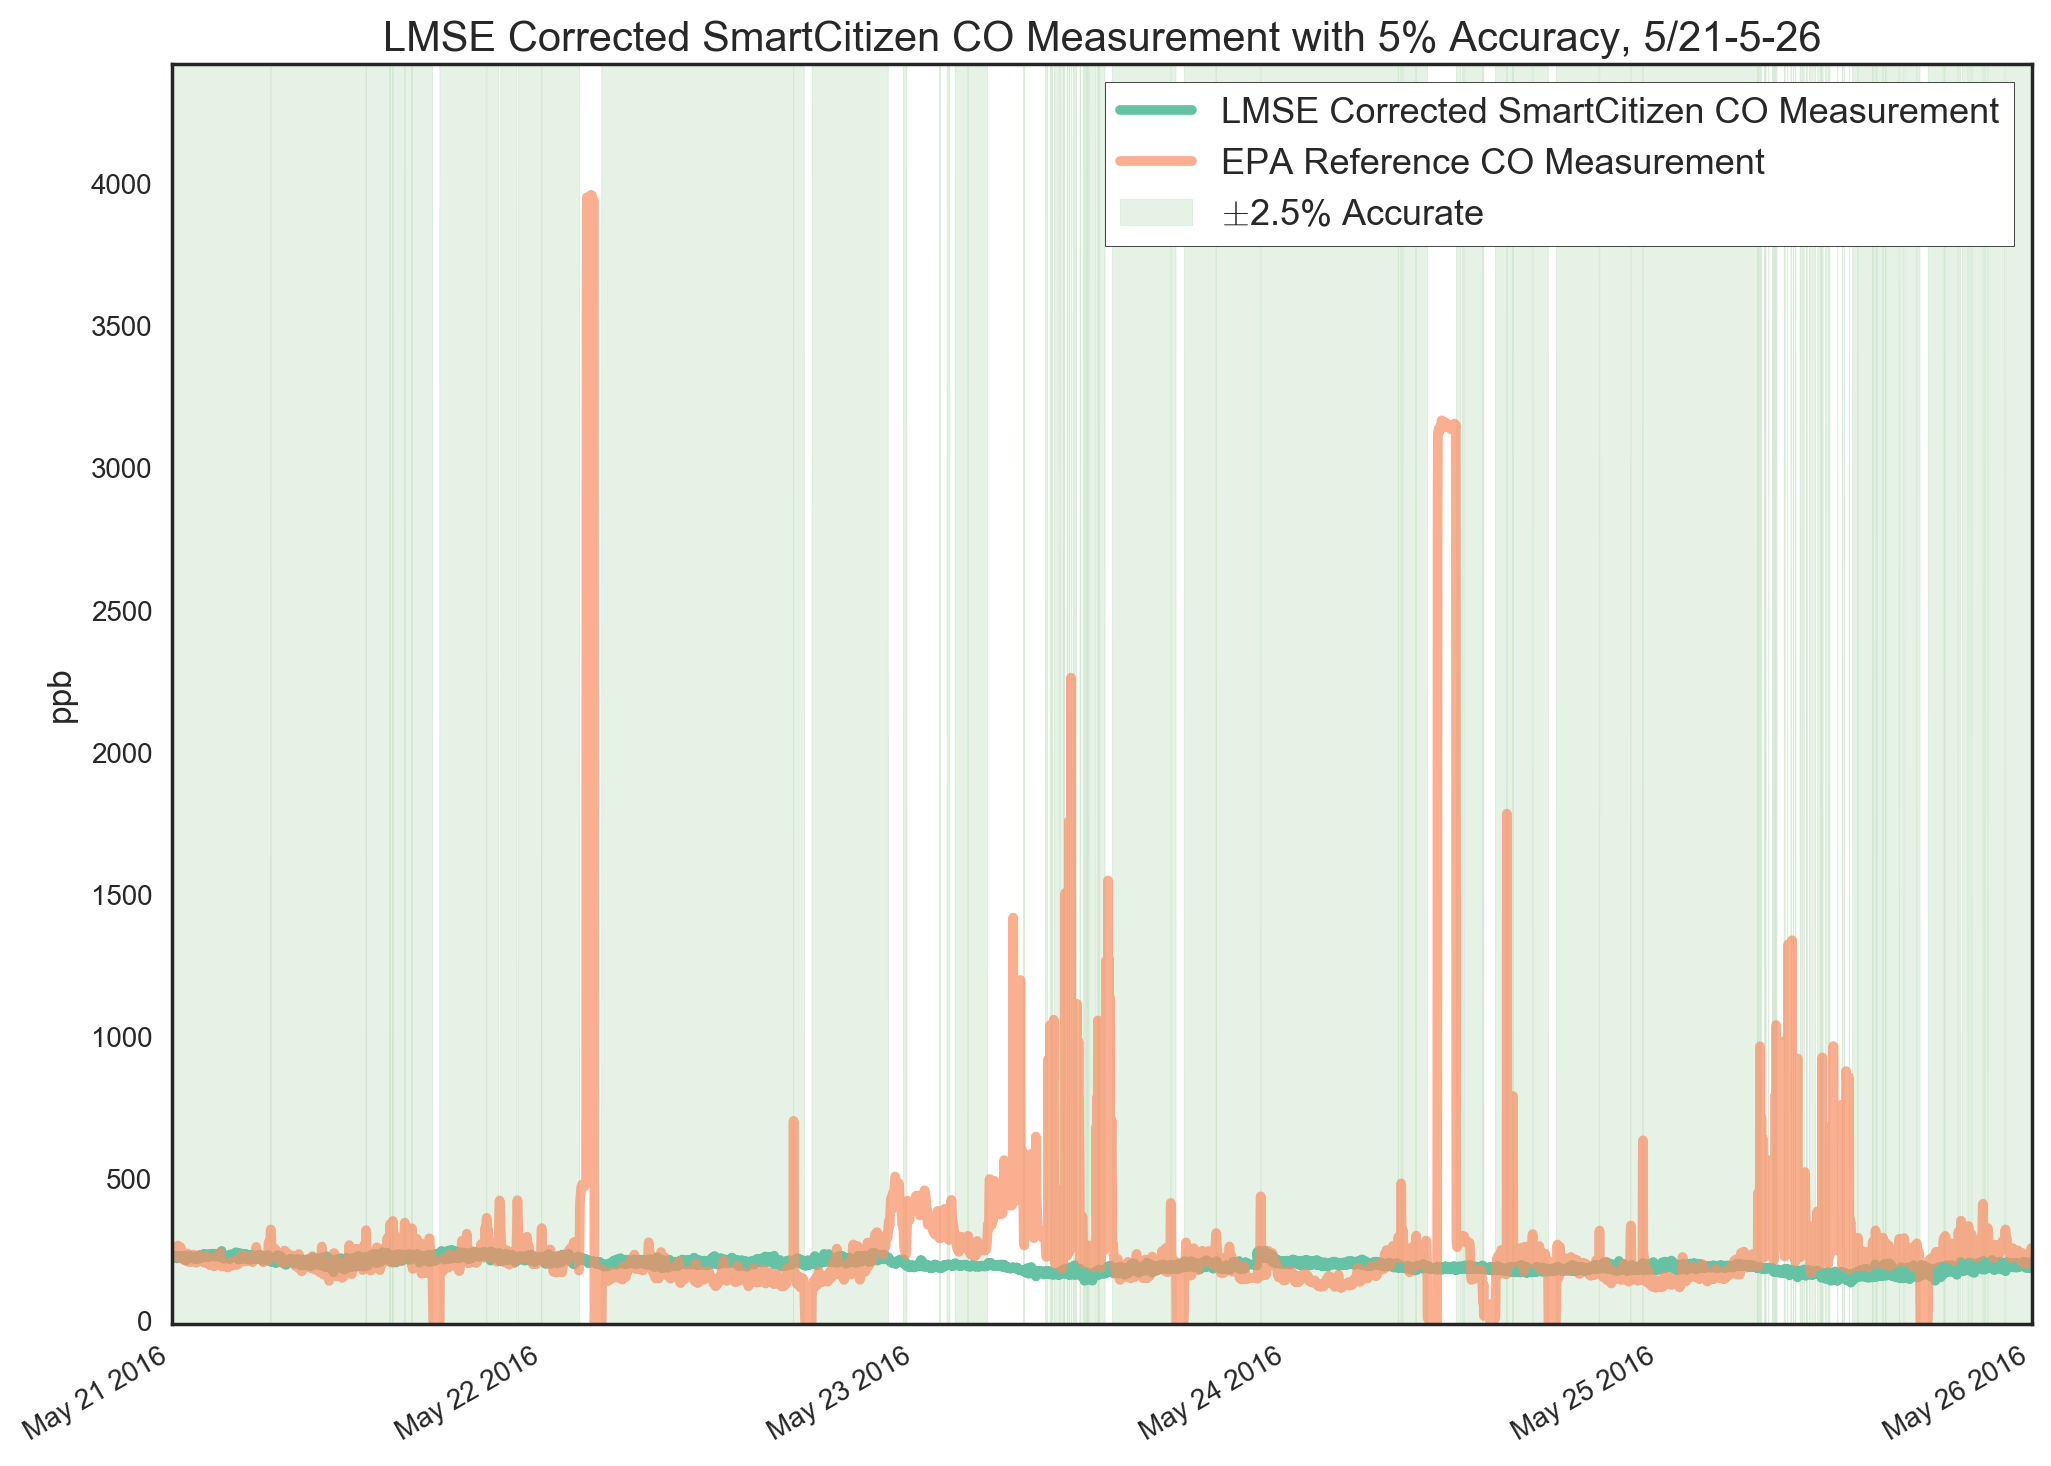
\includegraphics[width=\textwidth]{figs/sck_co_with_5_accuracy_zoomed}               
 	 \caption{SmartCitizen CO with 5\% Accuracy Threshold}
  	\label{fig:sck_co_with_5_accuracy_zoomed}
\end{figure}

\begin{figure}[htb]
 	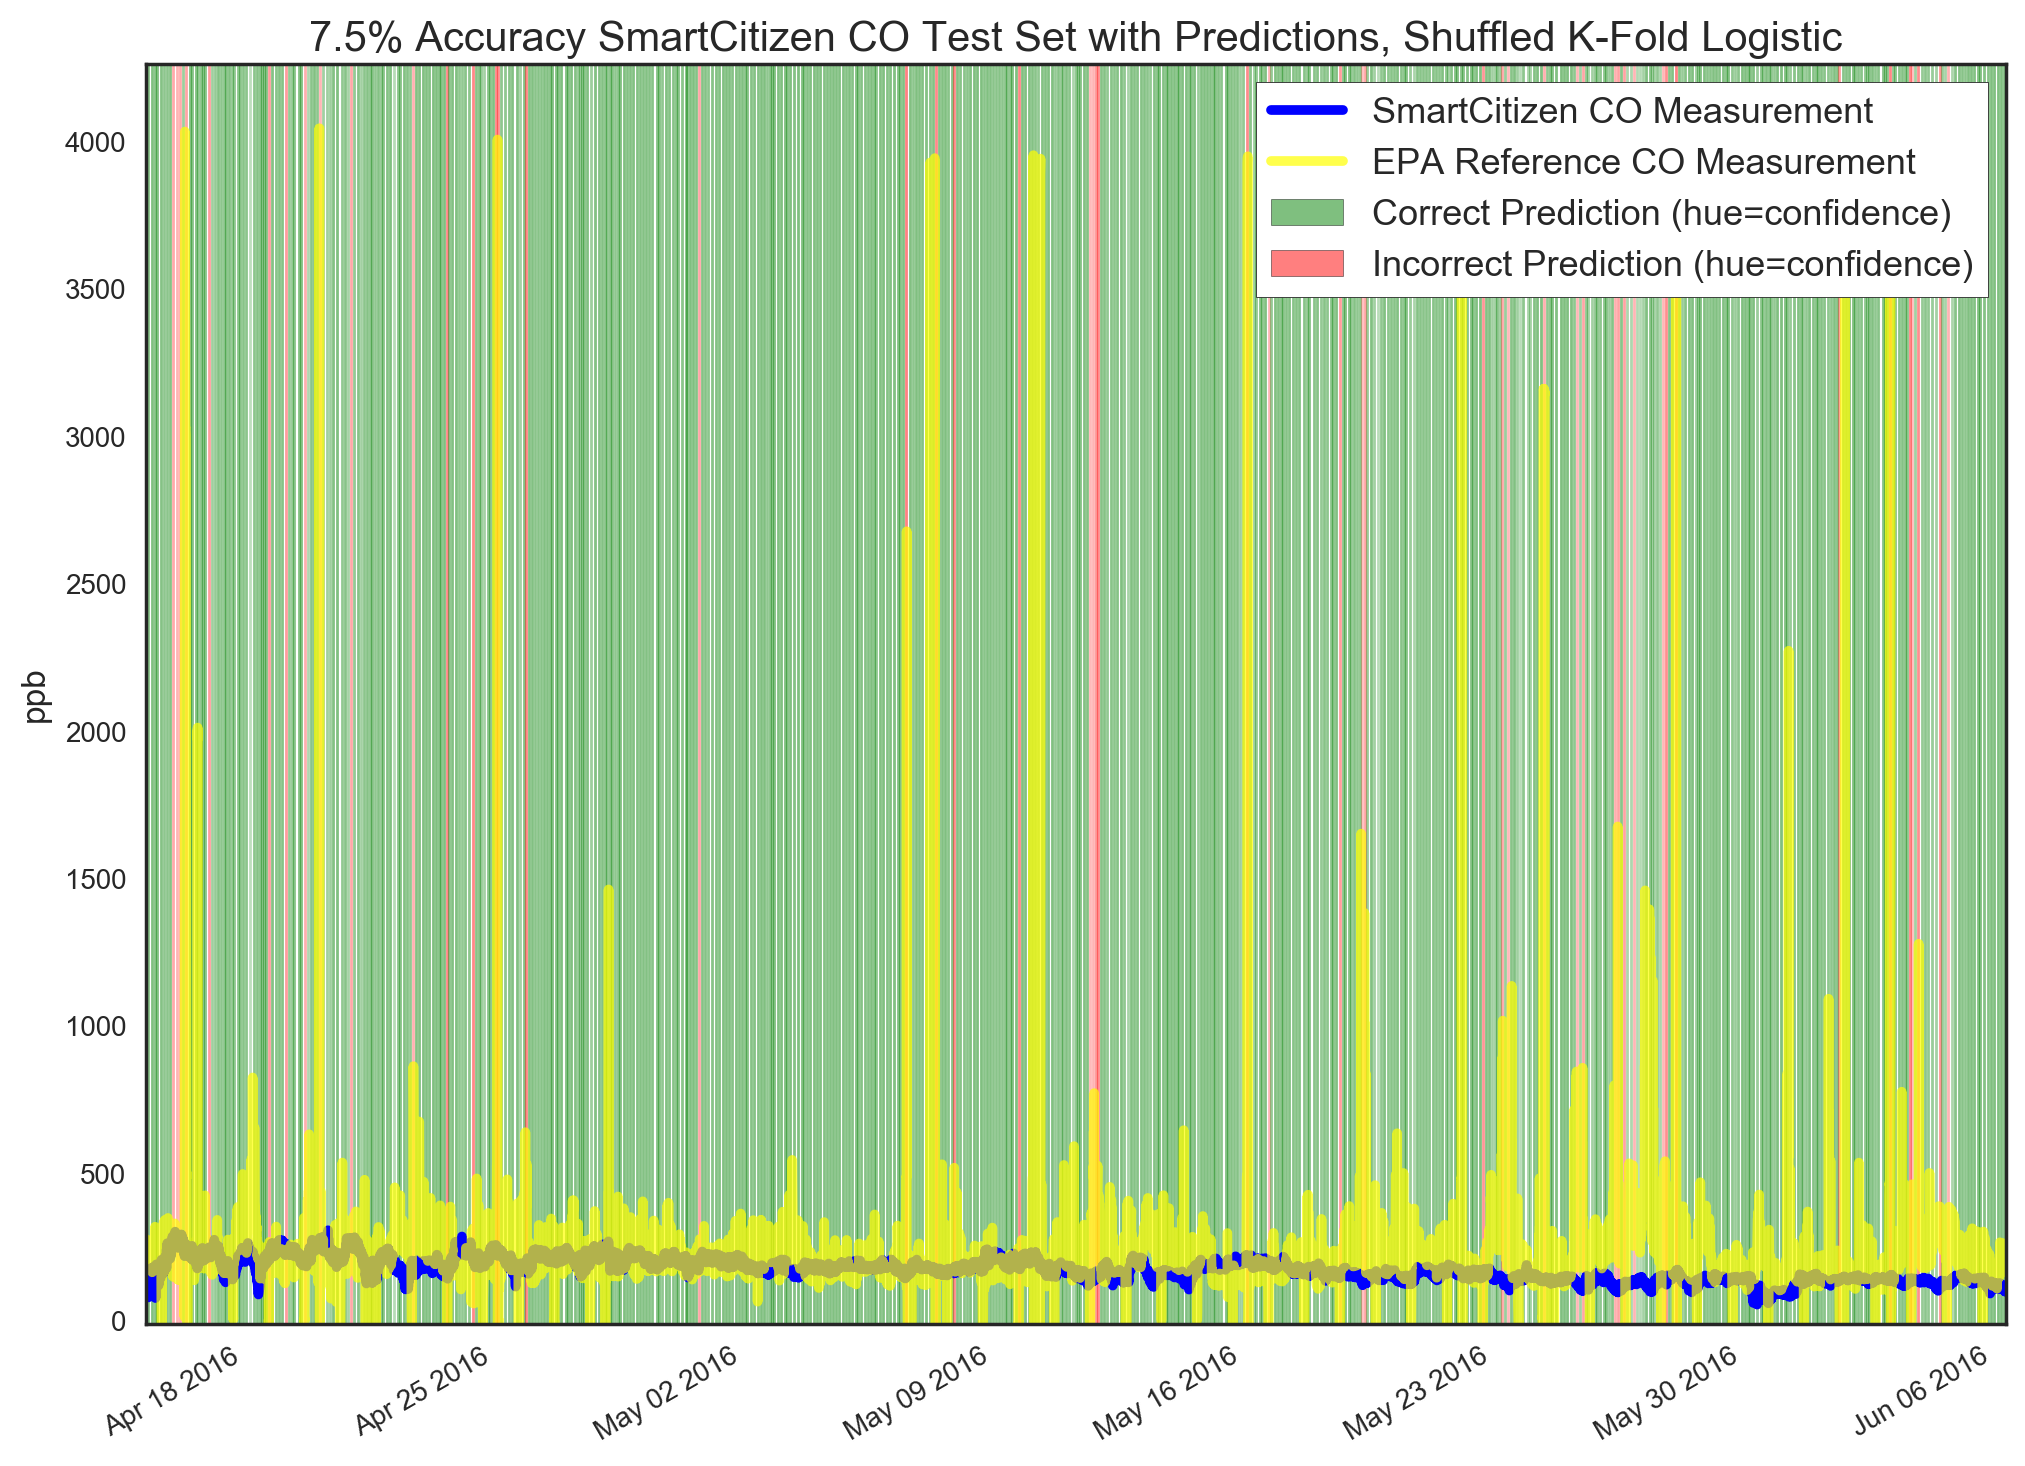
\includegraphics[width=\textwidth]{figs/sck_co_7p5_logistic_predictions}               
 	 \caption{SmartCitizen CO Prediction Accuracy}
  	\label{fig:sck_co_7p5_logistic_predictions}
\end{figure}

\begin{table}[H]
\centering
\begin{tabular}{lllllllll}
\\
\\
\toprule
Feature & Importance \\
\midrule
bkcarbon &  0.027481618644 \\
avg\_60\_bkcarbon &  0.0265308524121 \\
avg\_720\_bkcarbon &  0.0231734007362 \\
avg\_1440\_bkcarbon &  0.0213230536622 \\
avg\_60\_forecastio\_windSpeed &  0.0155772873357 \\
min\_since\_plugged\_in &  0.0151174982516 \\
temp\_sck\_box\_differential &  0.0148499597107 \\
avg\_60\_forecastio\_windBearing &  0.014573874136 \\
daily\_avg\_forecastio\_humidity &  0.0145367615821 \\
avg\_60\_forecastio\_dewPoint &  0.0138511147354 \\
avg\_60\_forecastio\_pressure &  0.0138476329536 \\
daily\_avg\_sck\_temperature &  0.0138353139286 \\
avg\_30\_ws &  0.0136031033823 \\
daily\_avg\_sck\_humidity &  0.0135231176757 \\
avg\_720\_lmse\_scaled\_sharpDust &  0.0132885608127 \\
\bottomrule
\end{tabular}
\label{tab:as1_co_randomforest_features}
\caption{Top 15 Features from Random Forest for SmartCitizen CO, used in Pruned Logistic Regression}
\end{table}

\begin{figure}[htb]
 	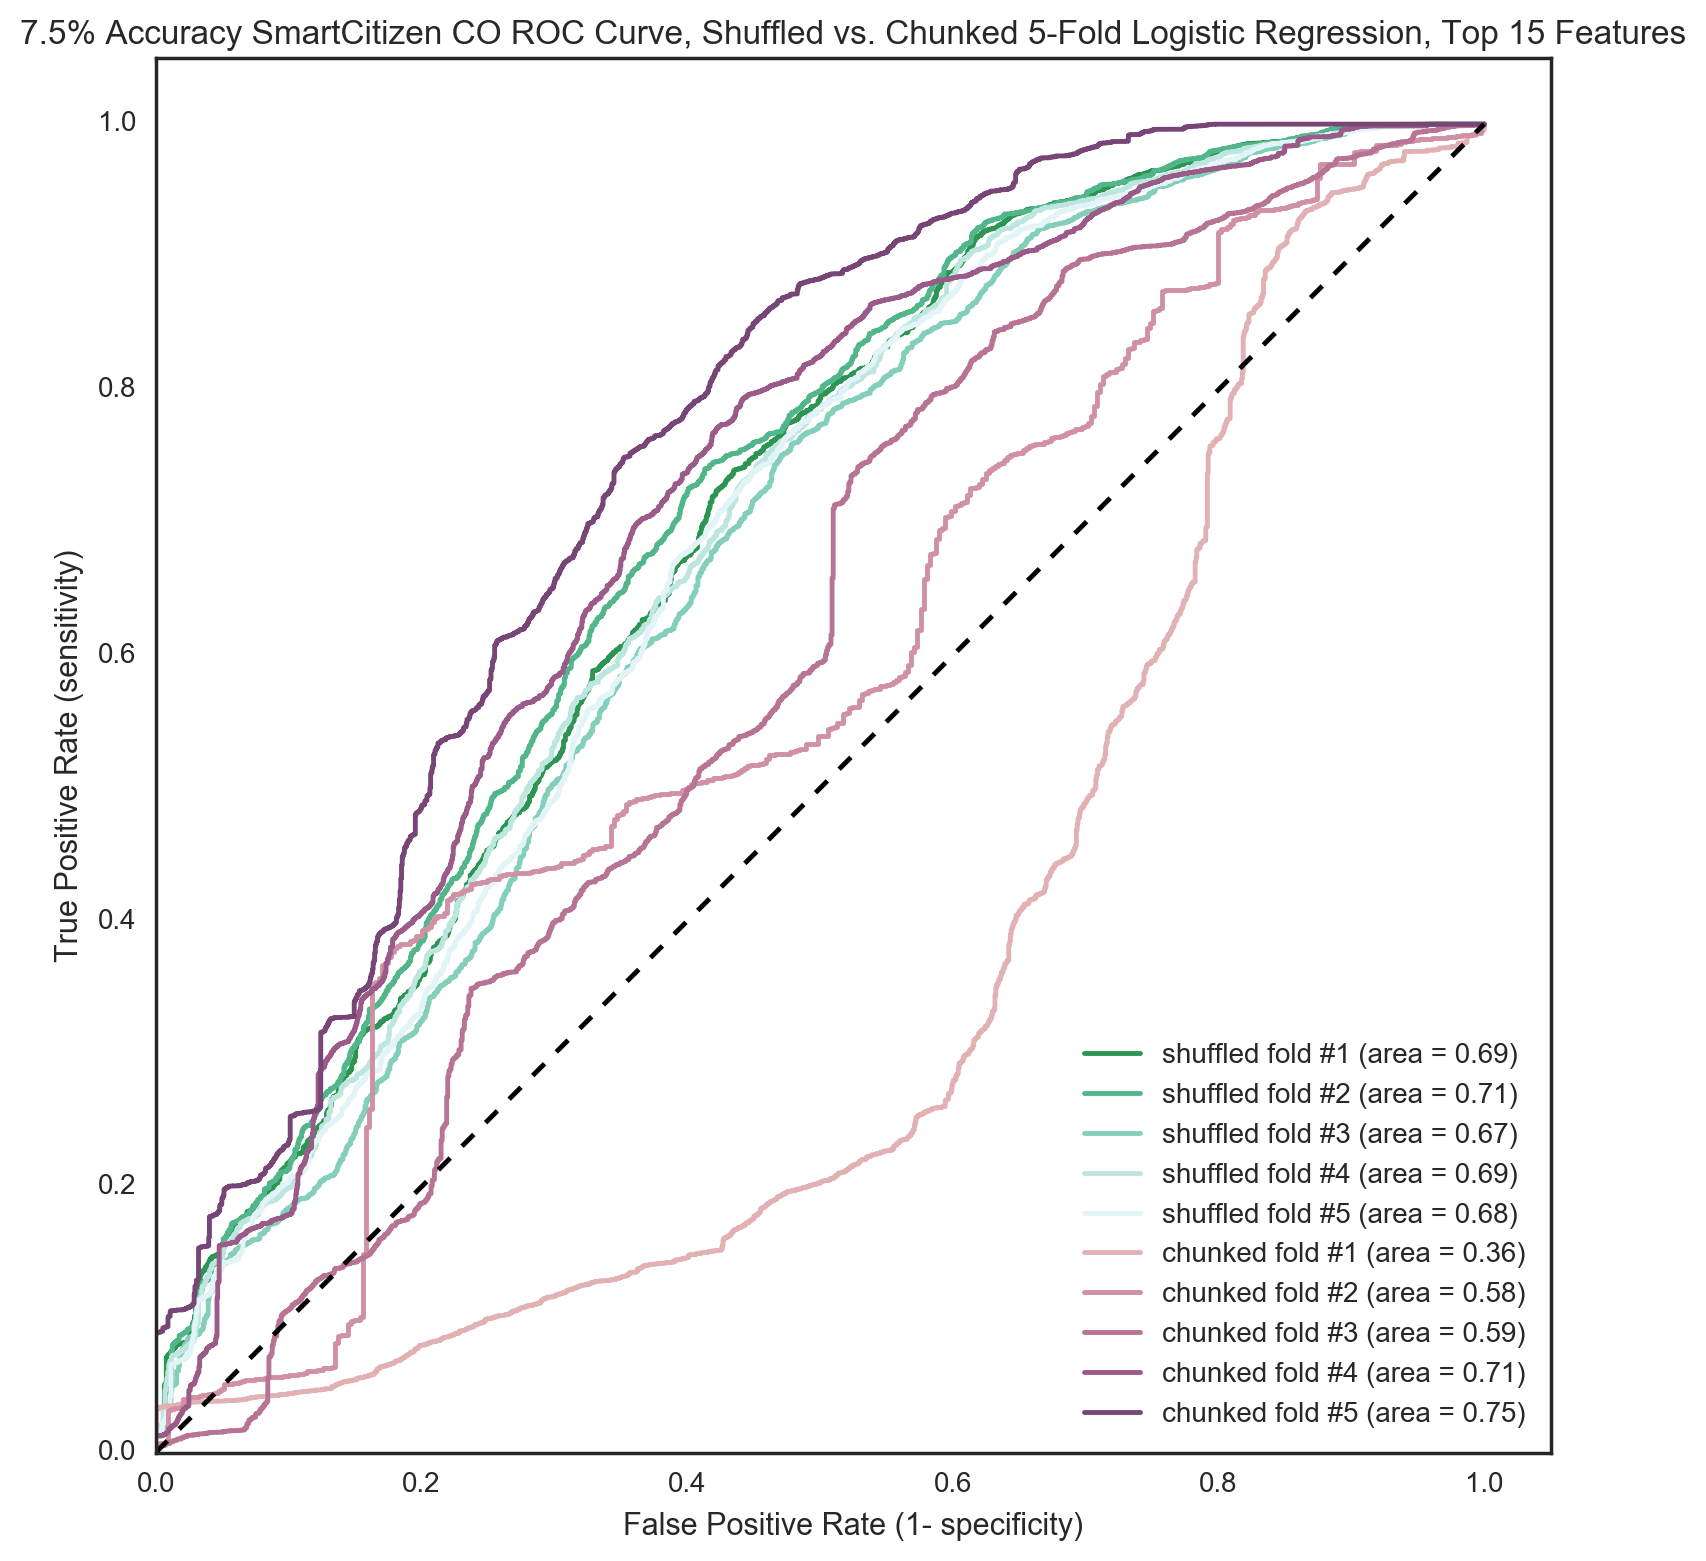
\includegraphics[width=\textwidth]{figs/sck_co_7p5_roc_pruned_features}               
 	 \caption{SmartCitizen CO ROC Using Top 15 Features}
  	\label{fig:sck_co_7p5_roc_pruned_features}
\end{figure}

\FloatBarrier
\section{SmartCitizen NO2}
\FloatBarrier

Following are additional plots from the SmartCitizen NO2 test outlining in more detail the LMSE calibration, the accuracy with a tighter 4\% threshold, a visualization of the prediction accuracy and confidence, and the top 15 random forest selected features.

\begin{figure}[htb]
 	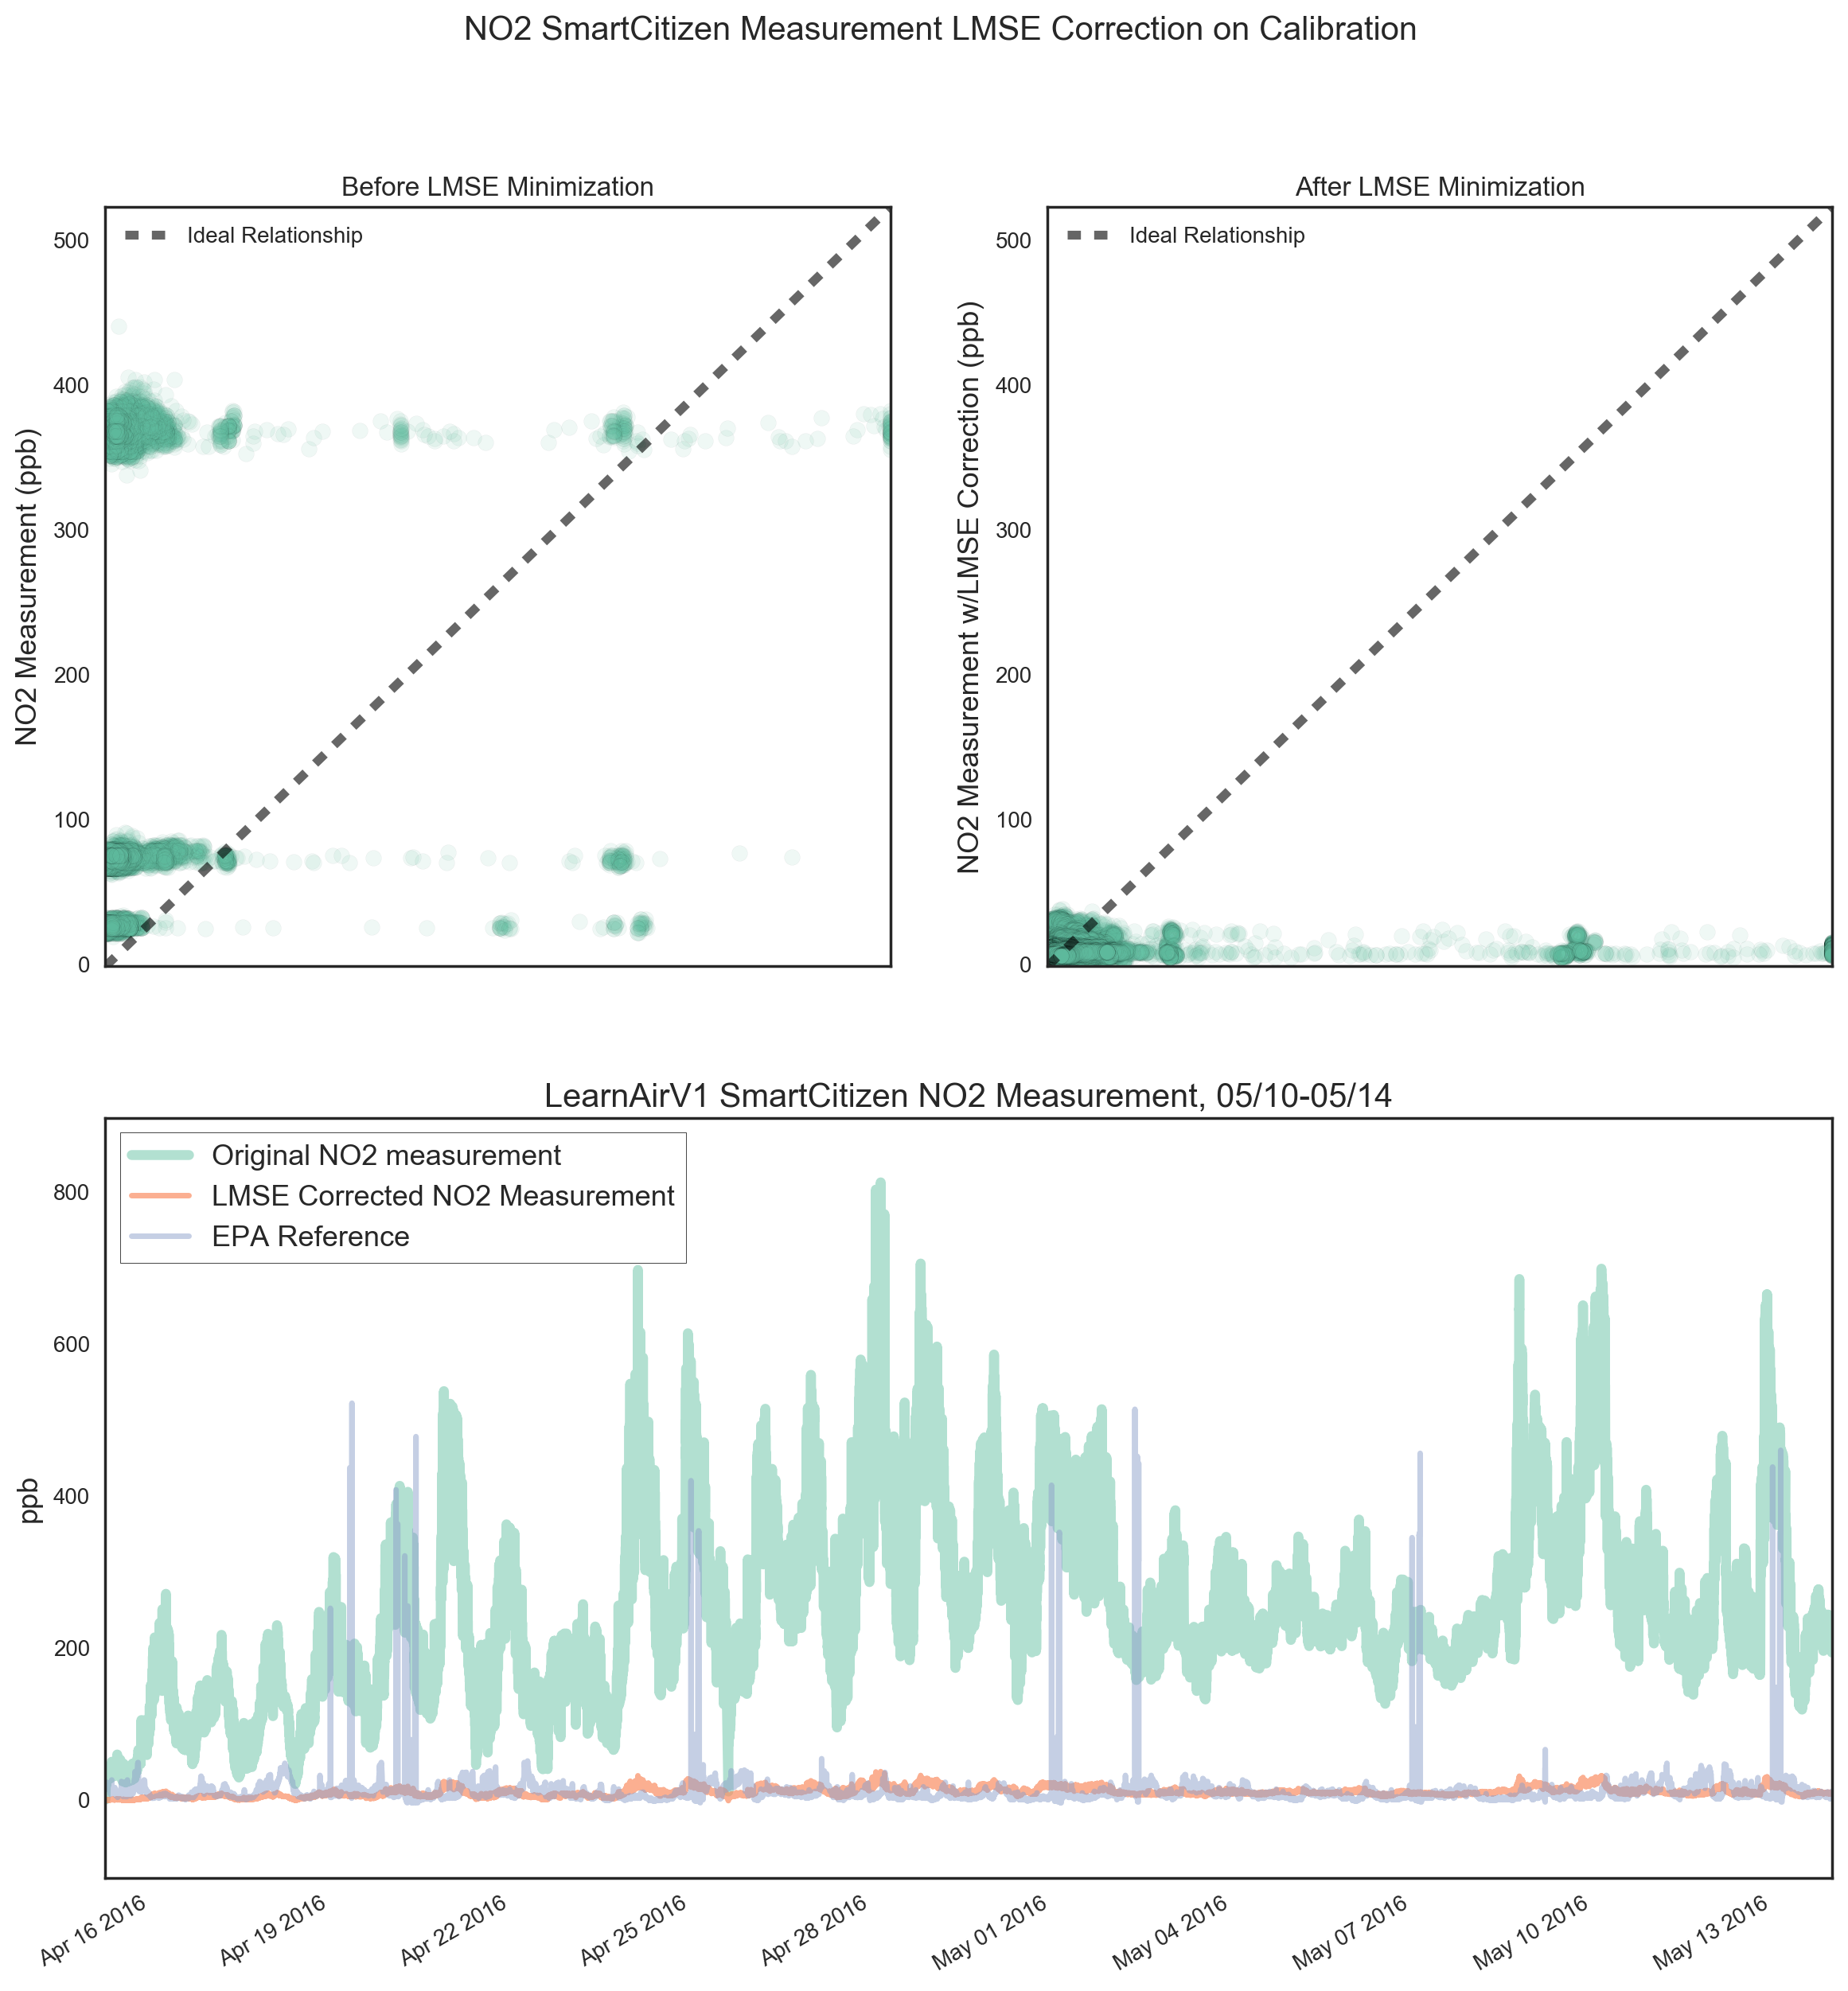
\includegraphics[width=\textwidth]{figs/sck_no2_lmse}               
 	 \caption{SmartCitizen NO2 after LMSE Calibration}
  	\label{fig:sck_no2_lmse}
\end{figure}

\begin{figure}[htb]
 	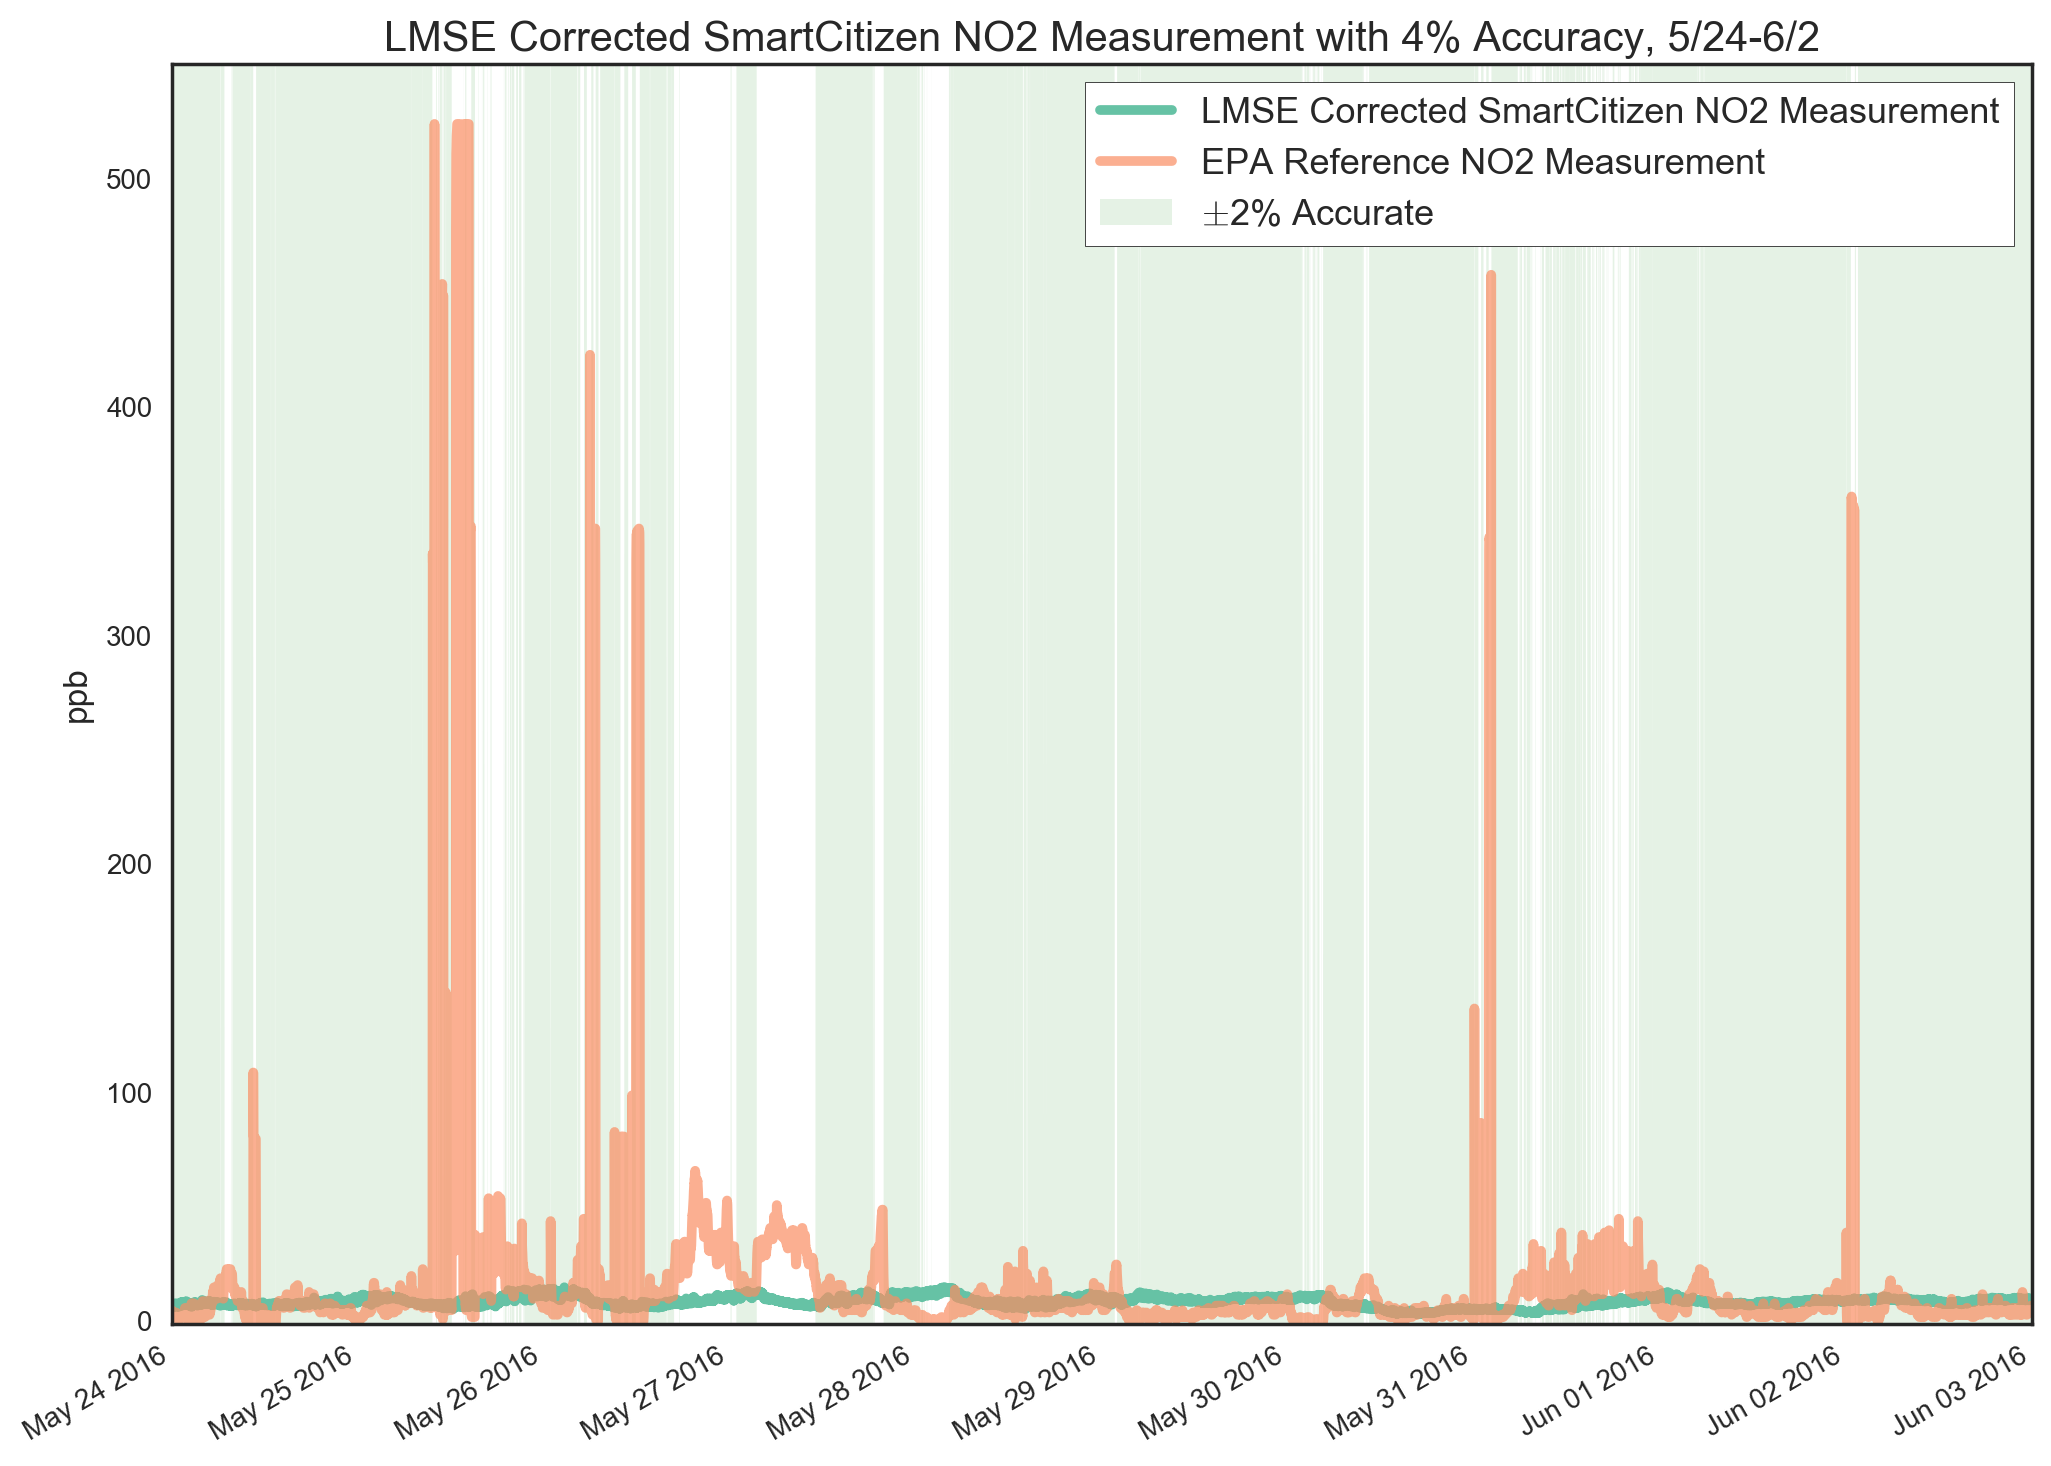
\includegraphics[width=\textwidth]{figs/sck_no2_with_4_accuracy_zoomed}               
 	 \caption{SmartCitizen NO2 with 4\% Accuracy Threshold}
  	\label{fig:sck_no2_with_4_accuracy_zoomed}
\end{figure}

\begin{figure}[htb]
 	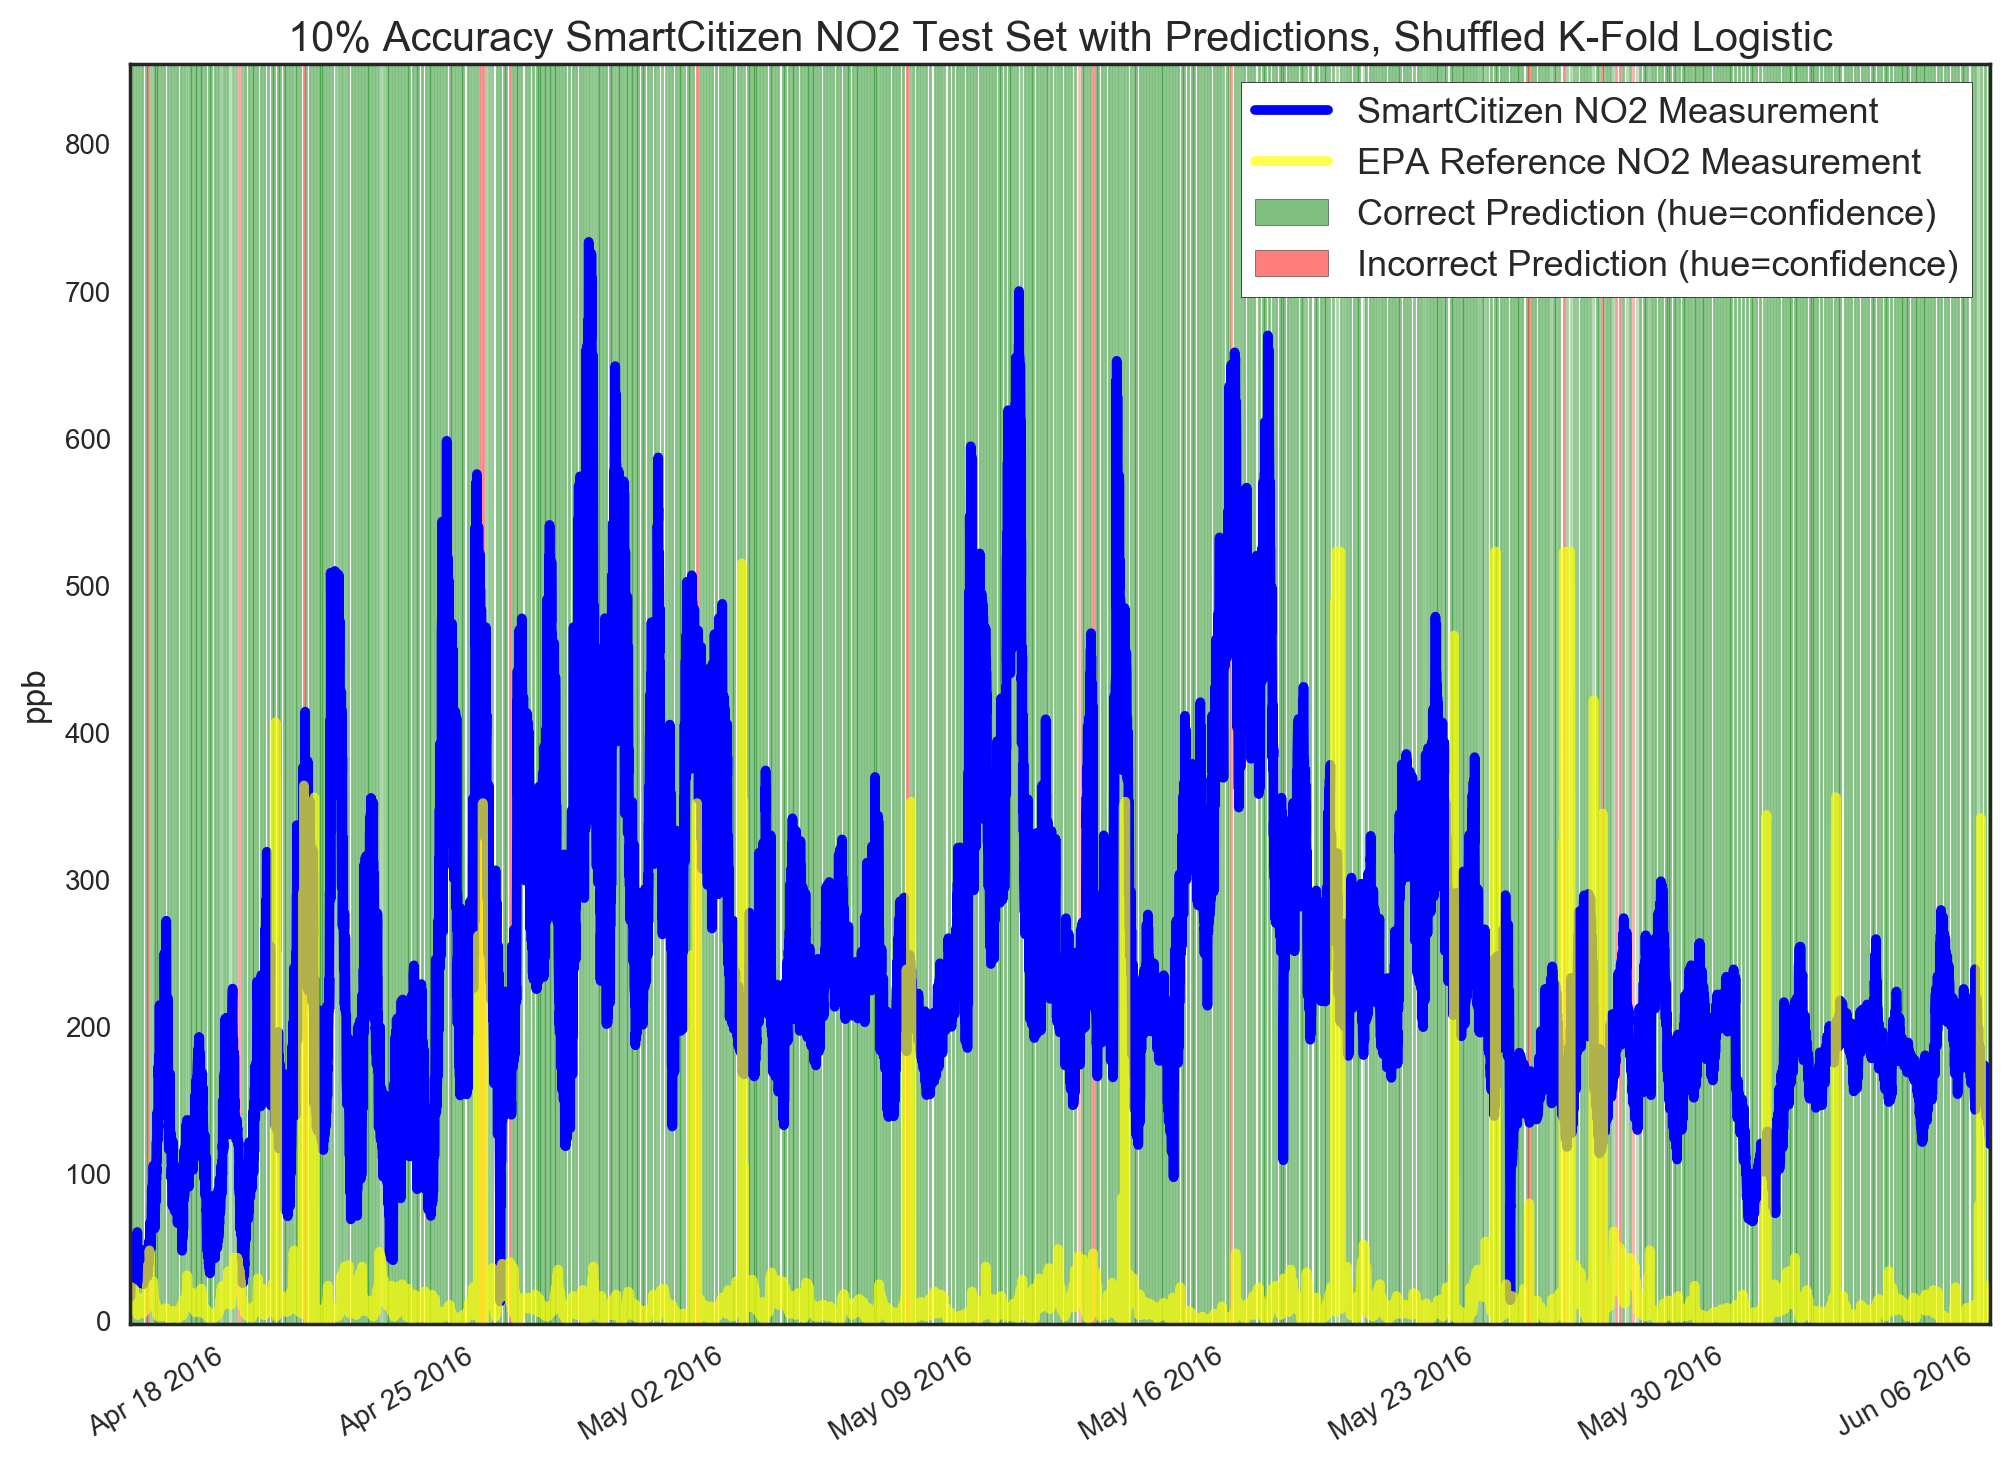
\includegraphics[width=\textwidth]{figs/sck_no2_10_logistic_predictions}               
 	 \caption{SmartCitizen NO2 Prediction Accuracy}
  	\label{fig:sck_no2_10_logistic_predictions}
\end{figure}

\begin{table}[H]
\centering
\begin{tabular}{lllllllll}
\\
\\
\toprule
Feature & Importance \\
\midrule

bkcarbon & 0.0459890536212 \\
avg\_60\_bkcarbon & 0.0433384018273 \\
avg\_720\_bkcarbon & 0.024690468695 \\
avg\_1440\_bkcarbon & 0.0210702674105 \\
avg\_60\_forecastio\_windSpeed & 0.0207714428351 \\
min\_since\_plugged\_in & 0.0173782542533 \\
avg\_60\_forecastio\_windBearing & 0.0172875801677 \\
forecastio\_windSpeed & 0.0170176630128 \\
avg\_1440\_lmse\_calib\_as\_co & 0.0162266191466 \\
daily\_avg\_sck\_humidity & 0.0160827543221 \\
avg\_60\_forecastio\_pressure & 0.0157403595739 \\
avg\_720\_lmse\_scaled\_sharpDust & 0.0154263296837 \\
avg\_1440\_lmse\_scaled\_sharpDust & 0.0153038668128 \\
daily\_avg\_as\_temperature & 0.0151434934355 \\
daily\_avg\_forecastio\_temperature & 0.0148922895233 \\
\bottomrule
\end{tabular}
\label{tab:sck_no2_randomforest_features}
\caption{Top 15 Features from Random Forest for SmartCitizen NO2, used in Pruned Logistic Regression}
\end{table}

\begin{figure}[htb]
 	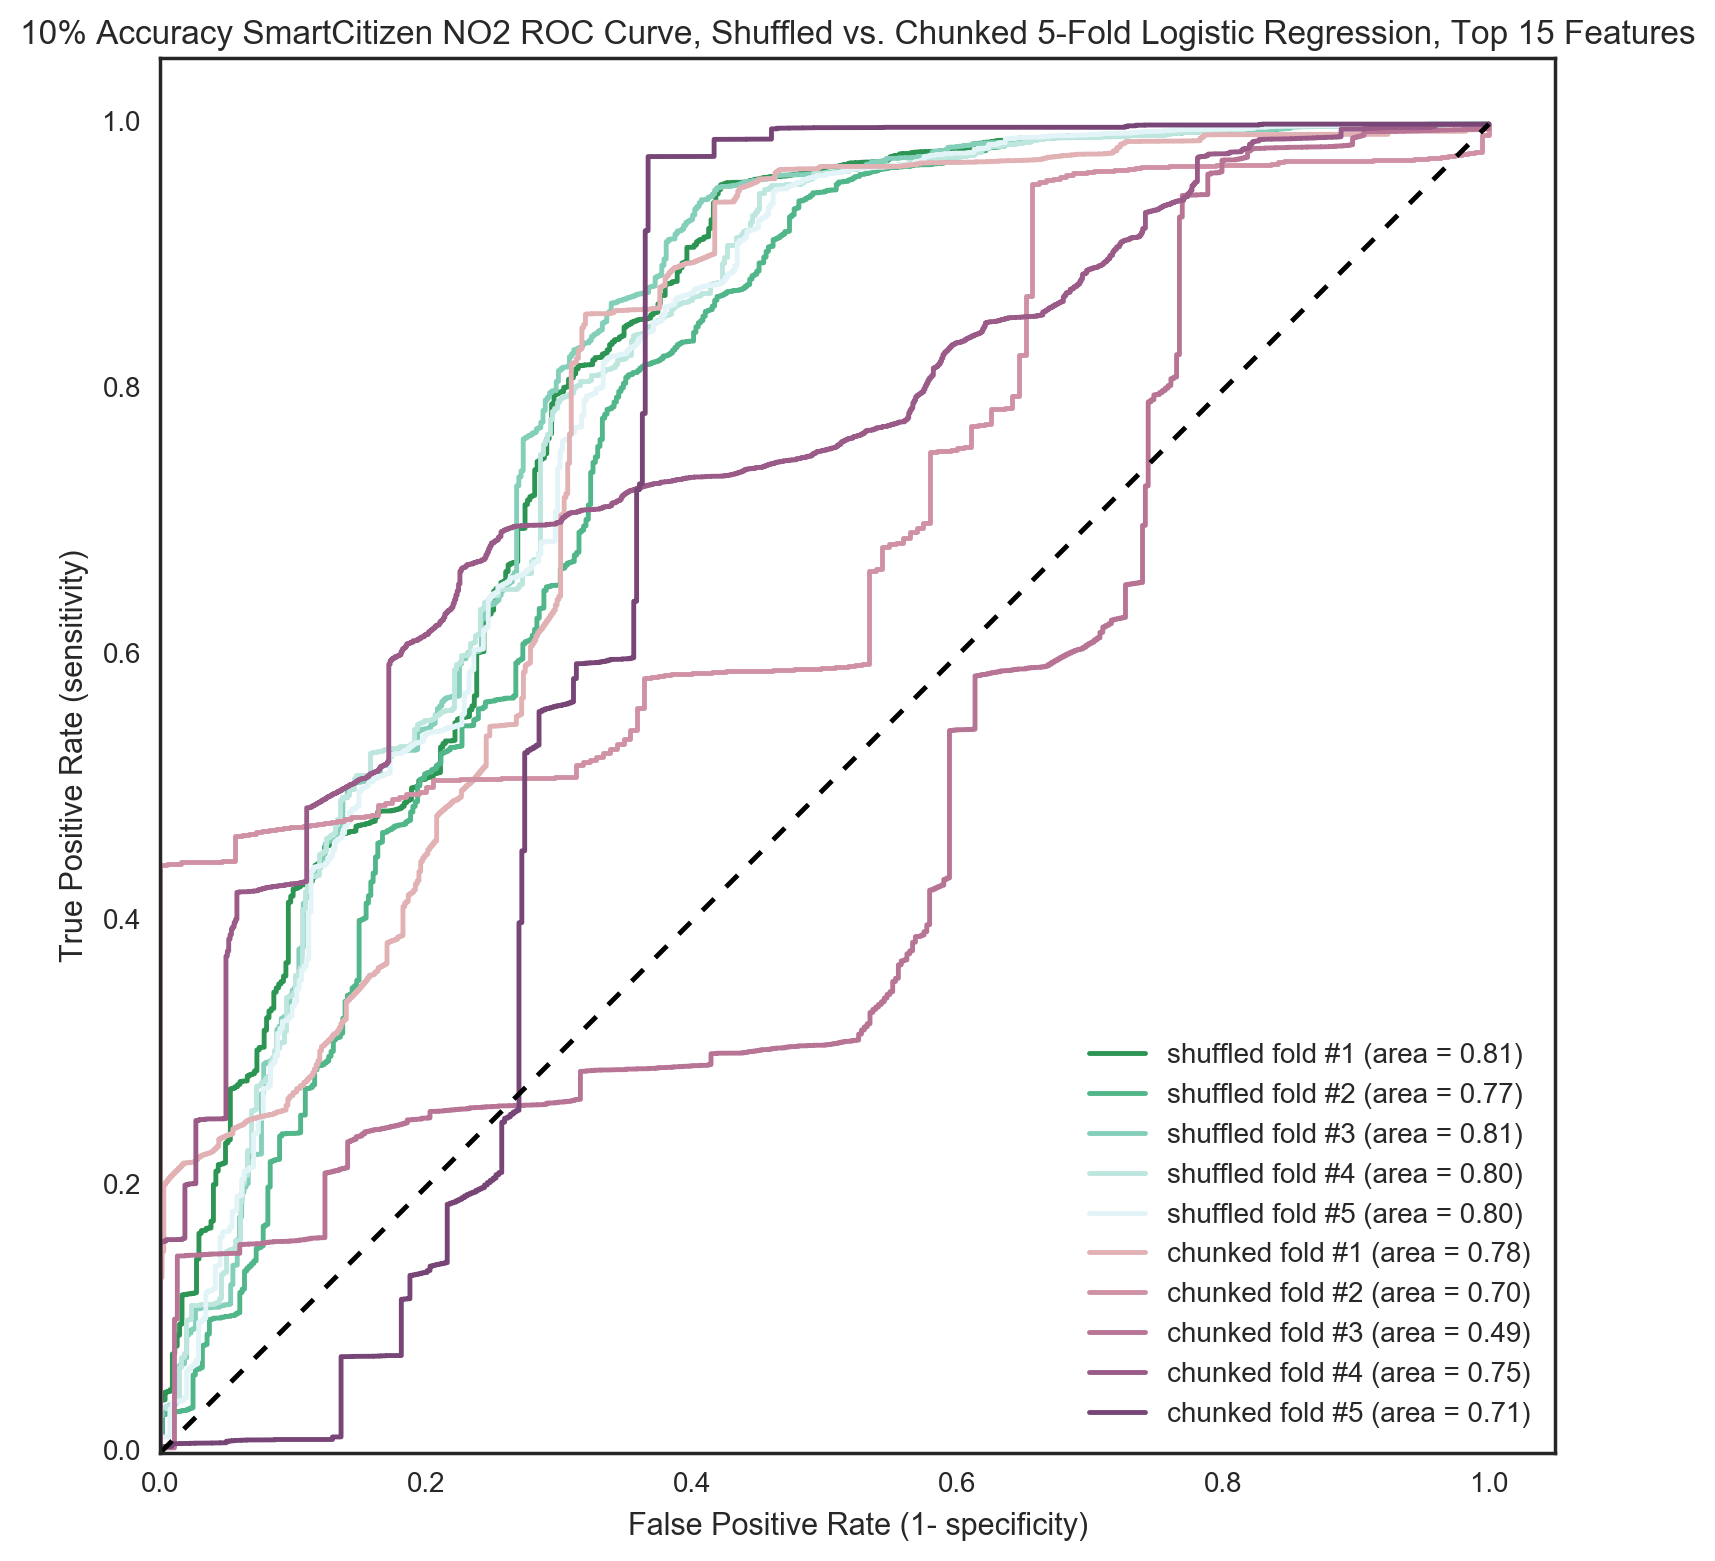
\includegraphics[width=\textwidth]{figs/sck_no2_10_roc_pruned_features}               
 	 \caption{SmartCitizen NO2 ROC Using Top 15 Features}
  	\label{fig:sck_no2_10_roc_pruned_features}
\end{figure}


\FloatBarrier
\section{Sharp Dust Sensor}
\FloatBarrier

Following are additional plots from the Sharp dust sensor test outlining the complete raw data, a visualization of the prediction accuracy and confidence, and the top 15 random forest selected features.

\begin{figure}[htb]
 	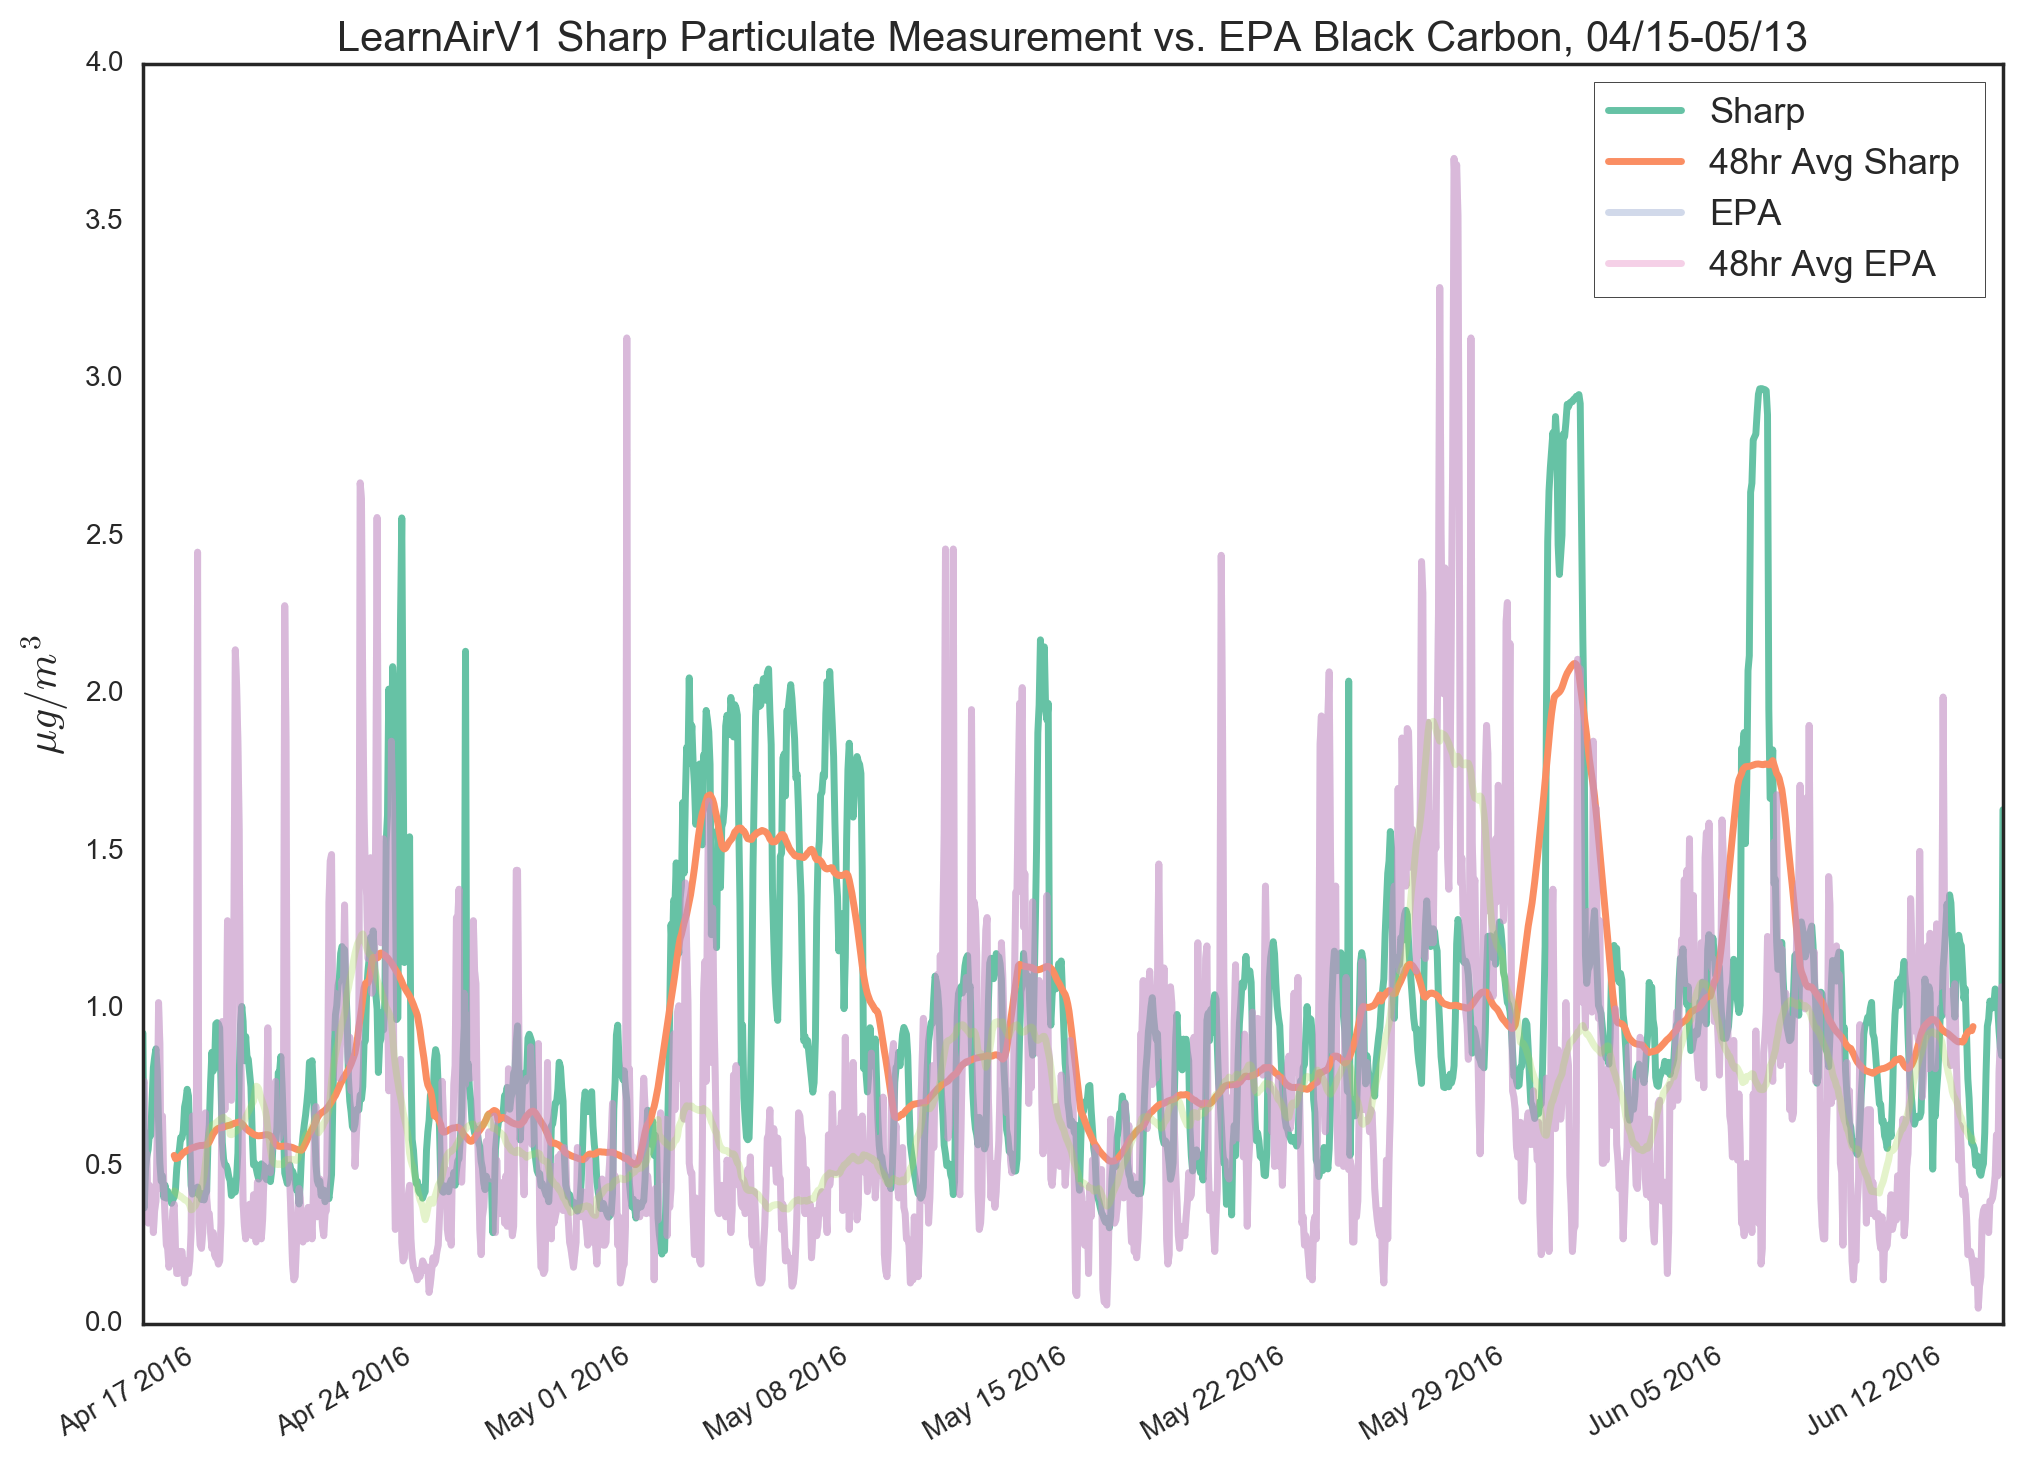
\includegraphics[width=\textwidth]{figs/sharp_raw}               
 	 \caption{Sharp Raw Particulate Data}
  	\label{fig:sharp_raw}
\end{figure}


\begin{figure}[htb]
 	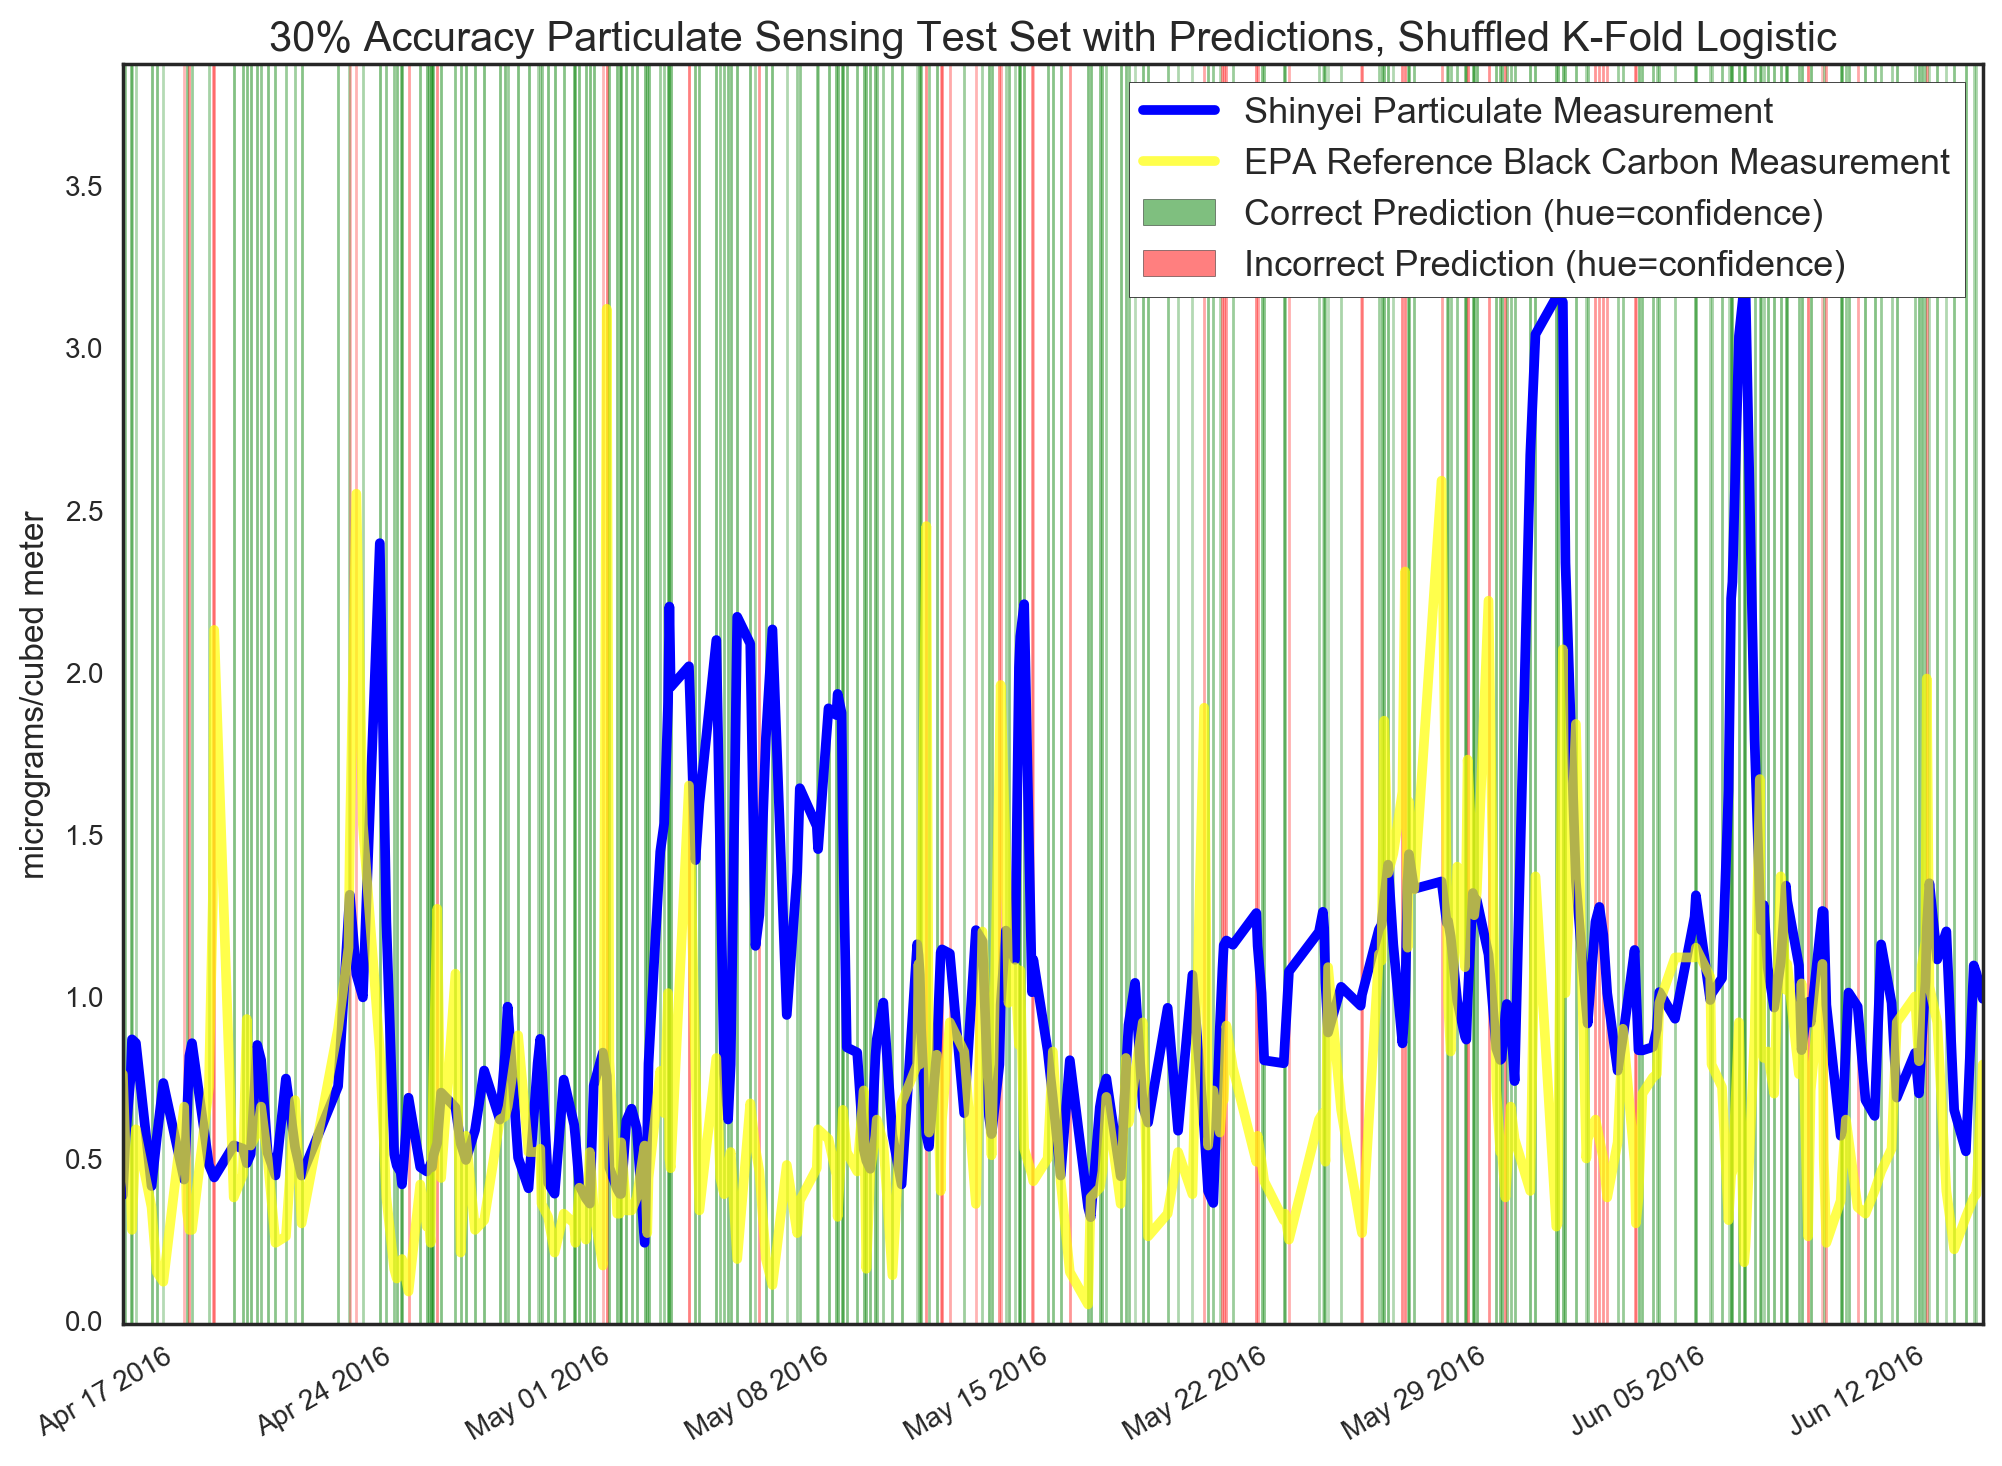
\includegraphics[width=\textwidth]{figs/sharp_goals_30_logistic_predictions}               
 	 \caption{Sharp Particulate Prediction Accuracy}
  	\label{fig:sharp_30_logistic_predictions}
\end{figure}

\begin{table}[H]
\centering
\begin{tabular}{lllllllll}
\\
\\
\toprule
Feature & Importance \\
\midrule
 scaled\_sharpDust &  0.039935725943 \\
 avg\_12\_scaled\_sharpDust &  0.0390147943972 \\
 sharpDust &  0.0390147211728 \\
 lmse\_scaled\_sharpDust &  0.0381632767126 \\
 avg\_48\_scaled\_sharpDust &  0.0225005941711 \\
 lmse\_avg\_48\_scaled\_sharpDust &  0.0207695248823 \\
 sck\_humidity &  0.0163292725576 \\
 Humidity ( \% RAW) &  0.0162400825573 \\
 no2 &  0.0149758603207 \\
 daily\_avg\_sck\_humidity &  0.0138699992039 \\
 daily\_avg\_forecastio\_humidity &  0.0132135840929 \\
 humidity\_box\_differential &  0.0119641893085 \\
 co &  0.0118968560369 \\
 sck\_humidity\_saturated &  0.0103888721788 \\
 avg\_60\_forecastio\_humidity &  0.0102980544091 \\
\bottomrule
\end{tabular}
\label{tab:sharp_randomforest_features}
\caption{Top 15 Features from Random Forest for Sharp Sensor, used in Pruned Logistic Regression}
\end{table}

Following are ROC curves for the Sharp sensor using just the top 15 features (for both the hour and 48 hour averaged data), as well as ROC curves and features for tighter tolerances (15\% instead of 30\% of full-scale).

\begin{figure}[htb]
 	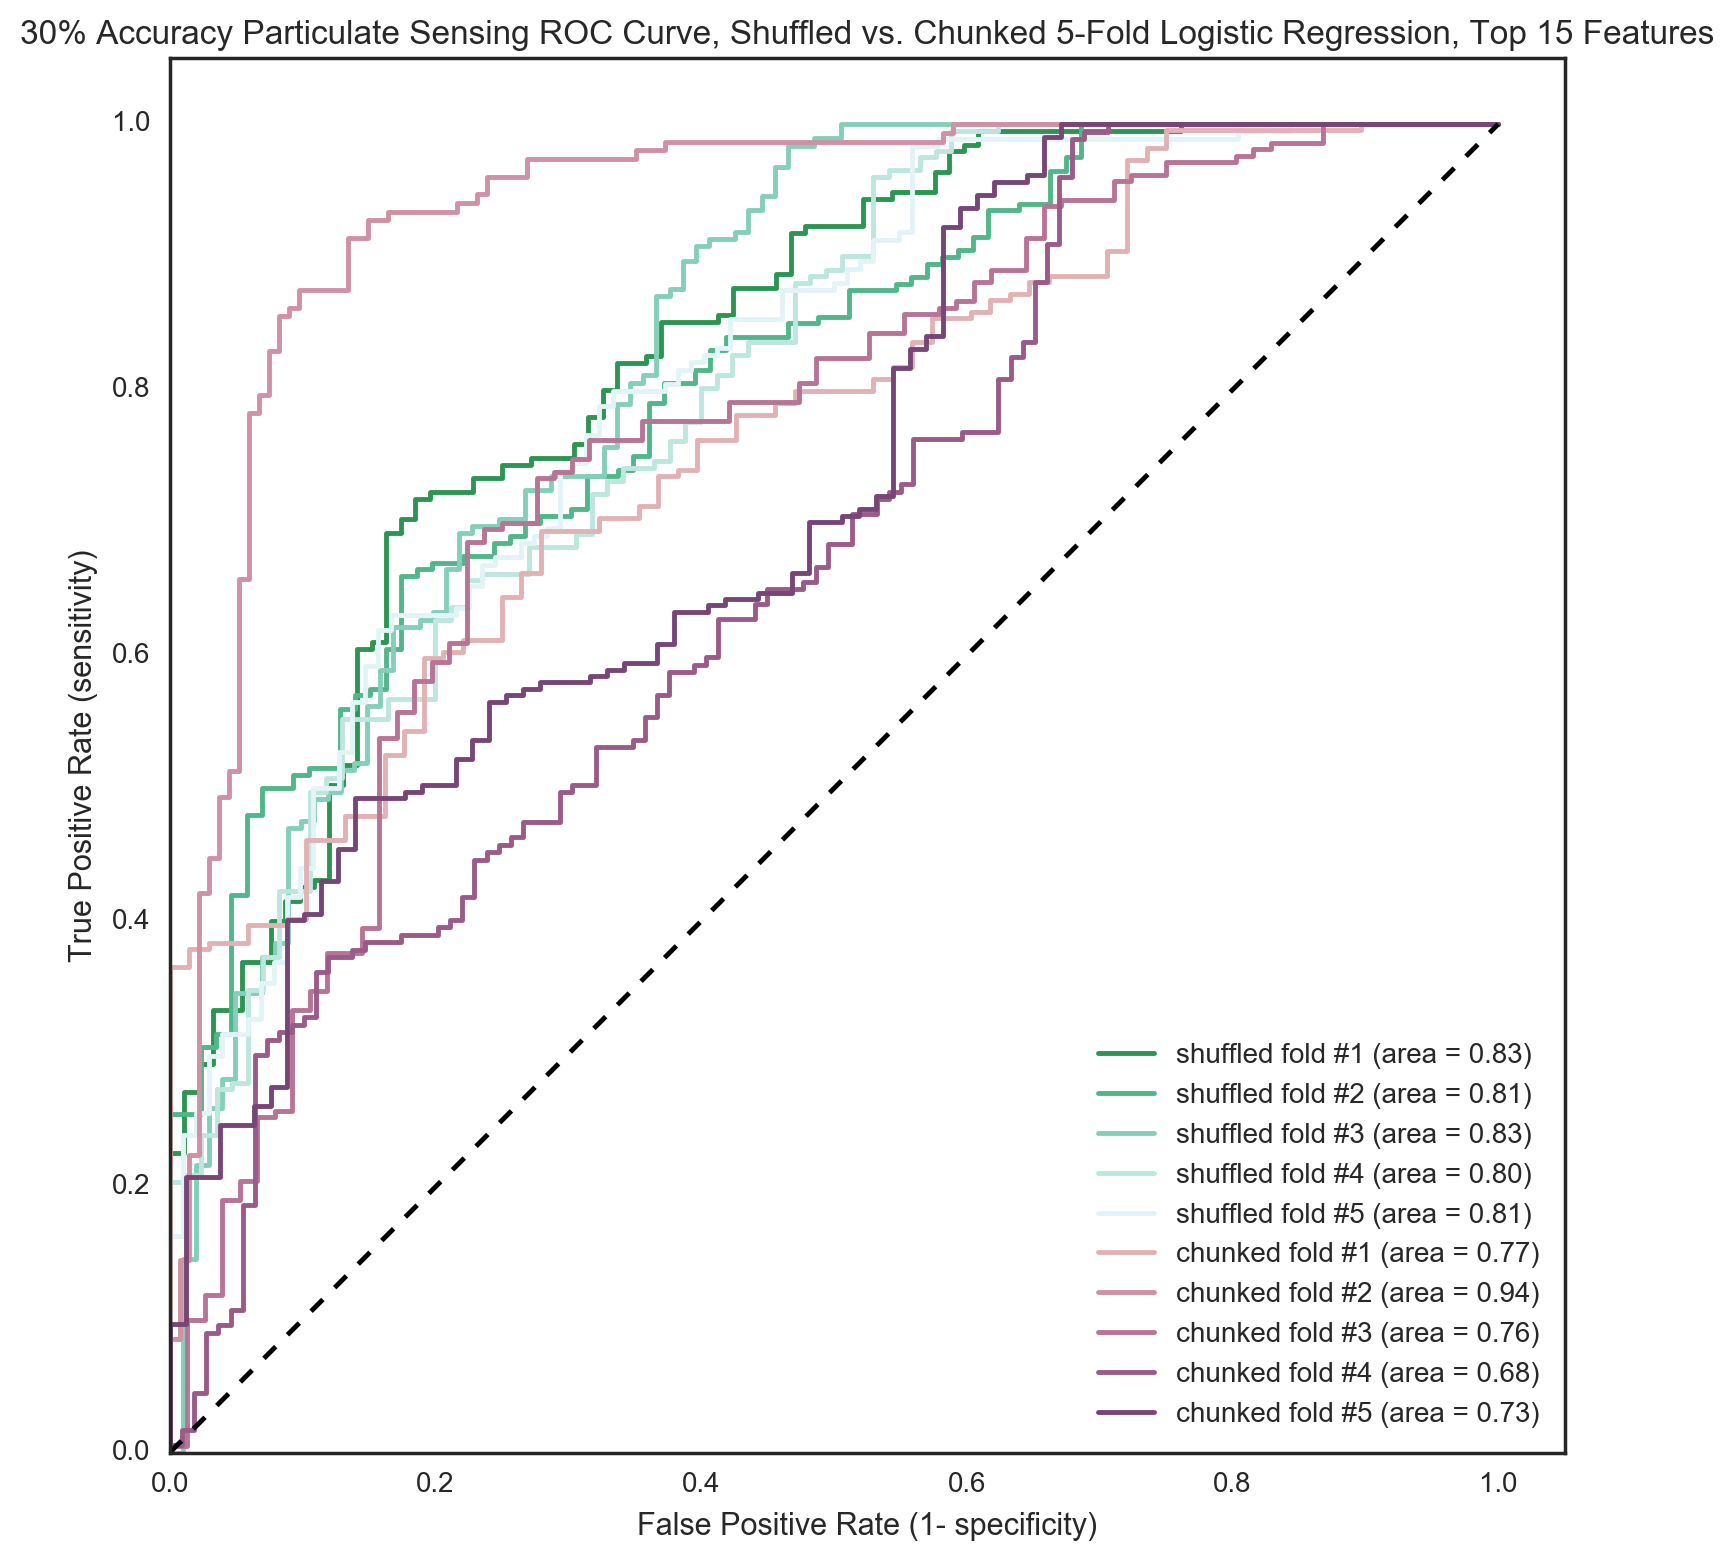
\includegraphics[width=\textwidth]{figs/sharp_goals_30_roc_pruned_features}               
 	 \caption{Sharp Particulate ROC Using Top 15 Features}
  	\label{fig:sharp_30_roc_pruned_features}
\end{figure}


\begin{figure}[htb]
 	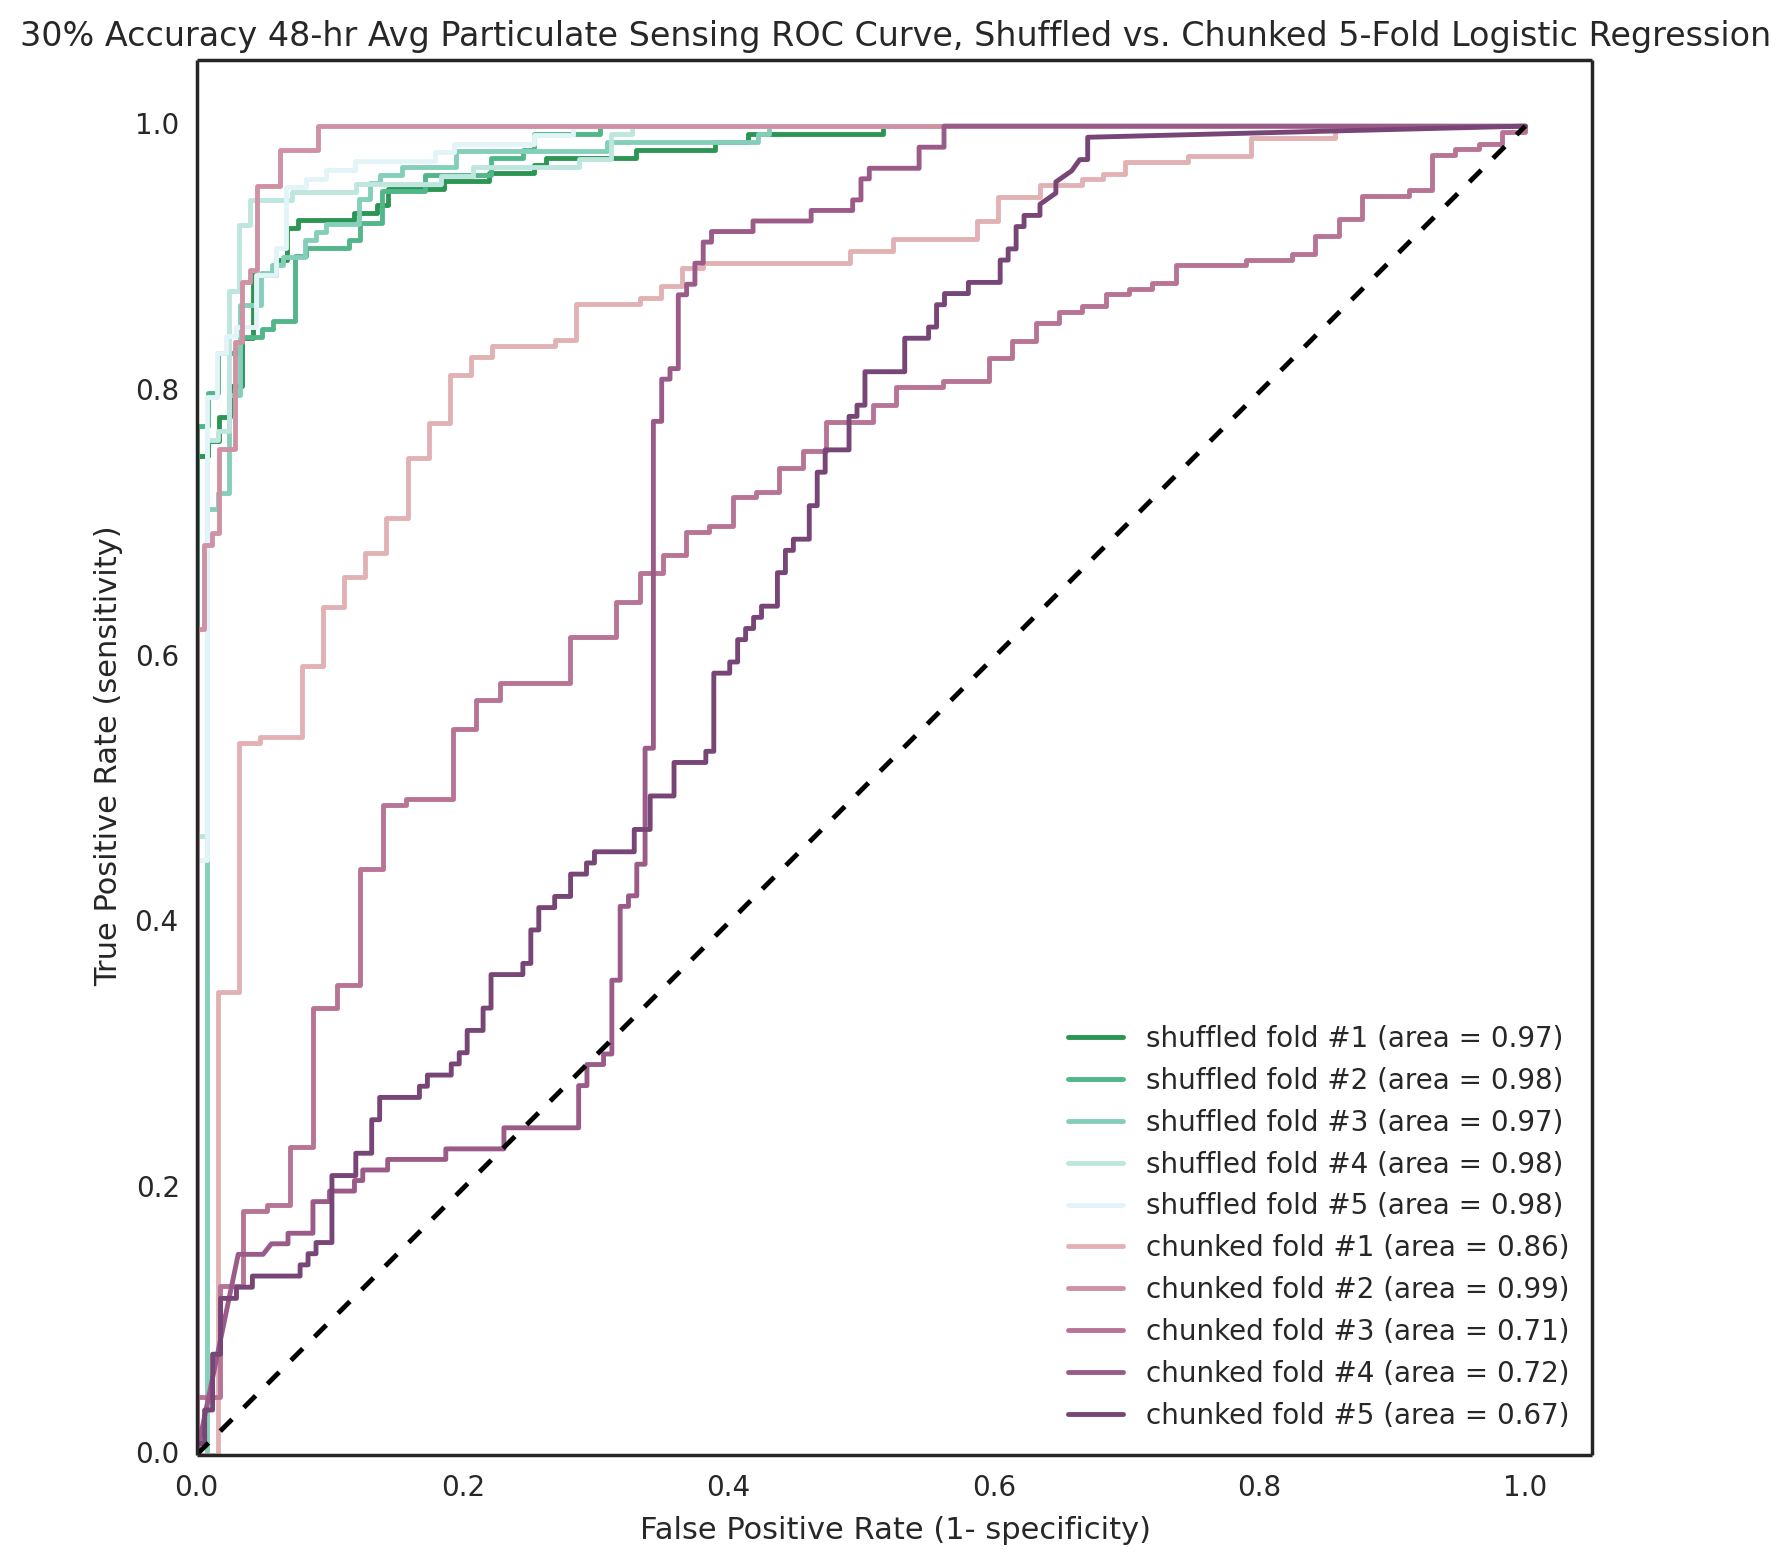
\includegraphics[width=\textwidth]{figs/sharp_48_avg_goals_30_roc}               
 	 \caption{48-hour Average Sharp Particulate ROC}
  	\label{fig:sharp_48_avg_goals_30_roc}
\end{figure}

\begin{figure}[htb]
 	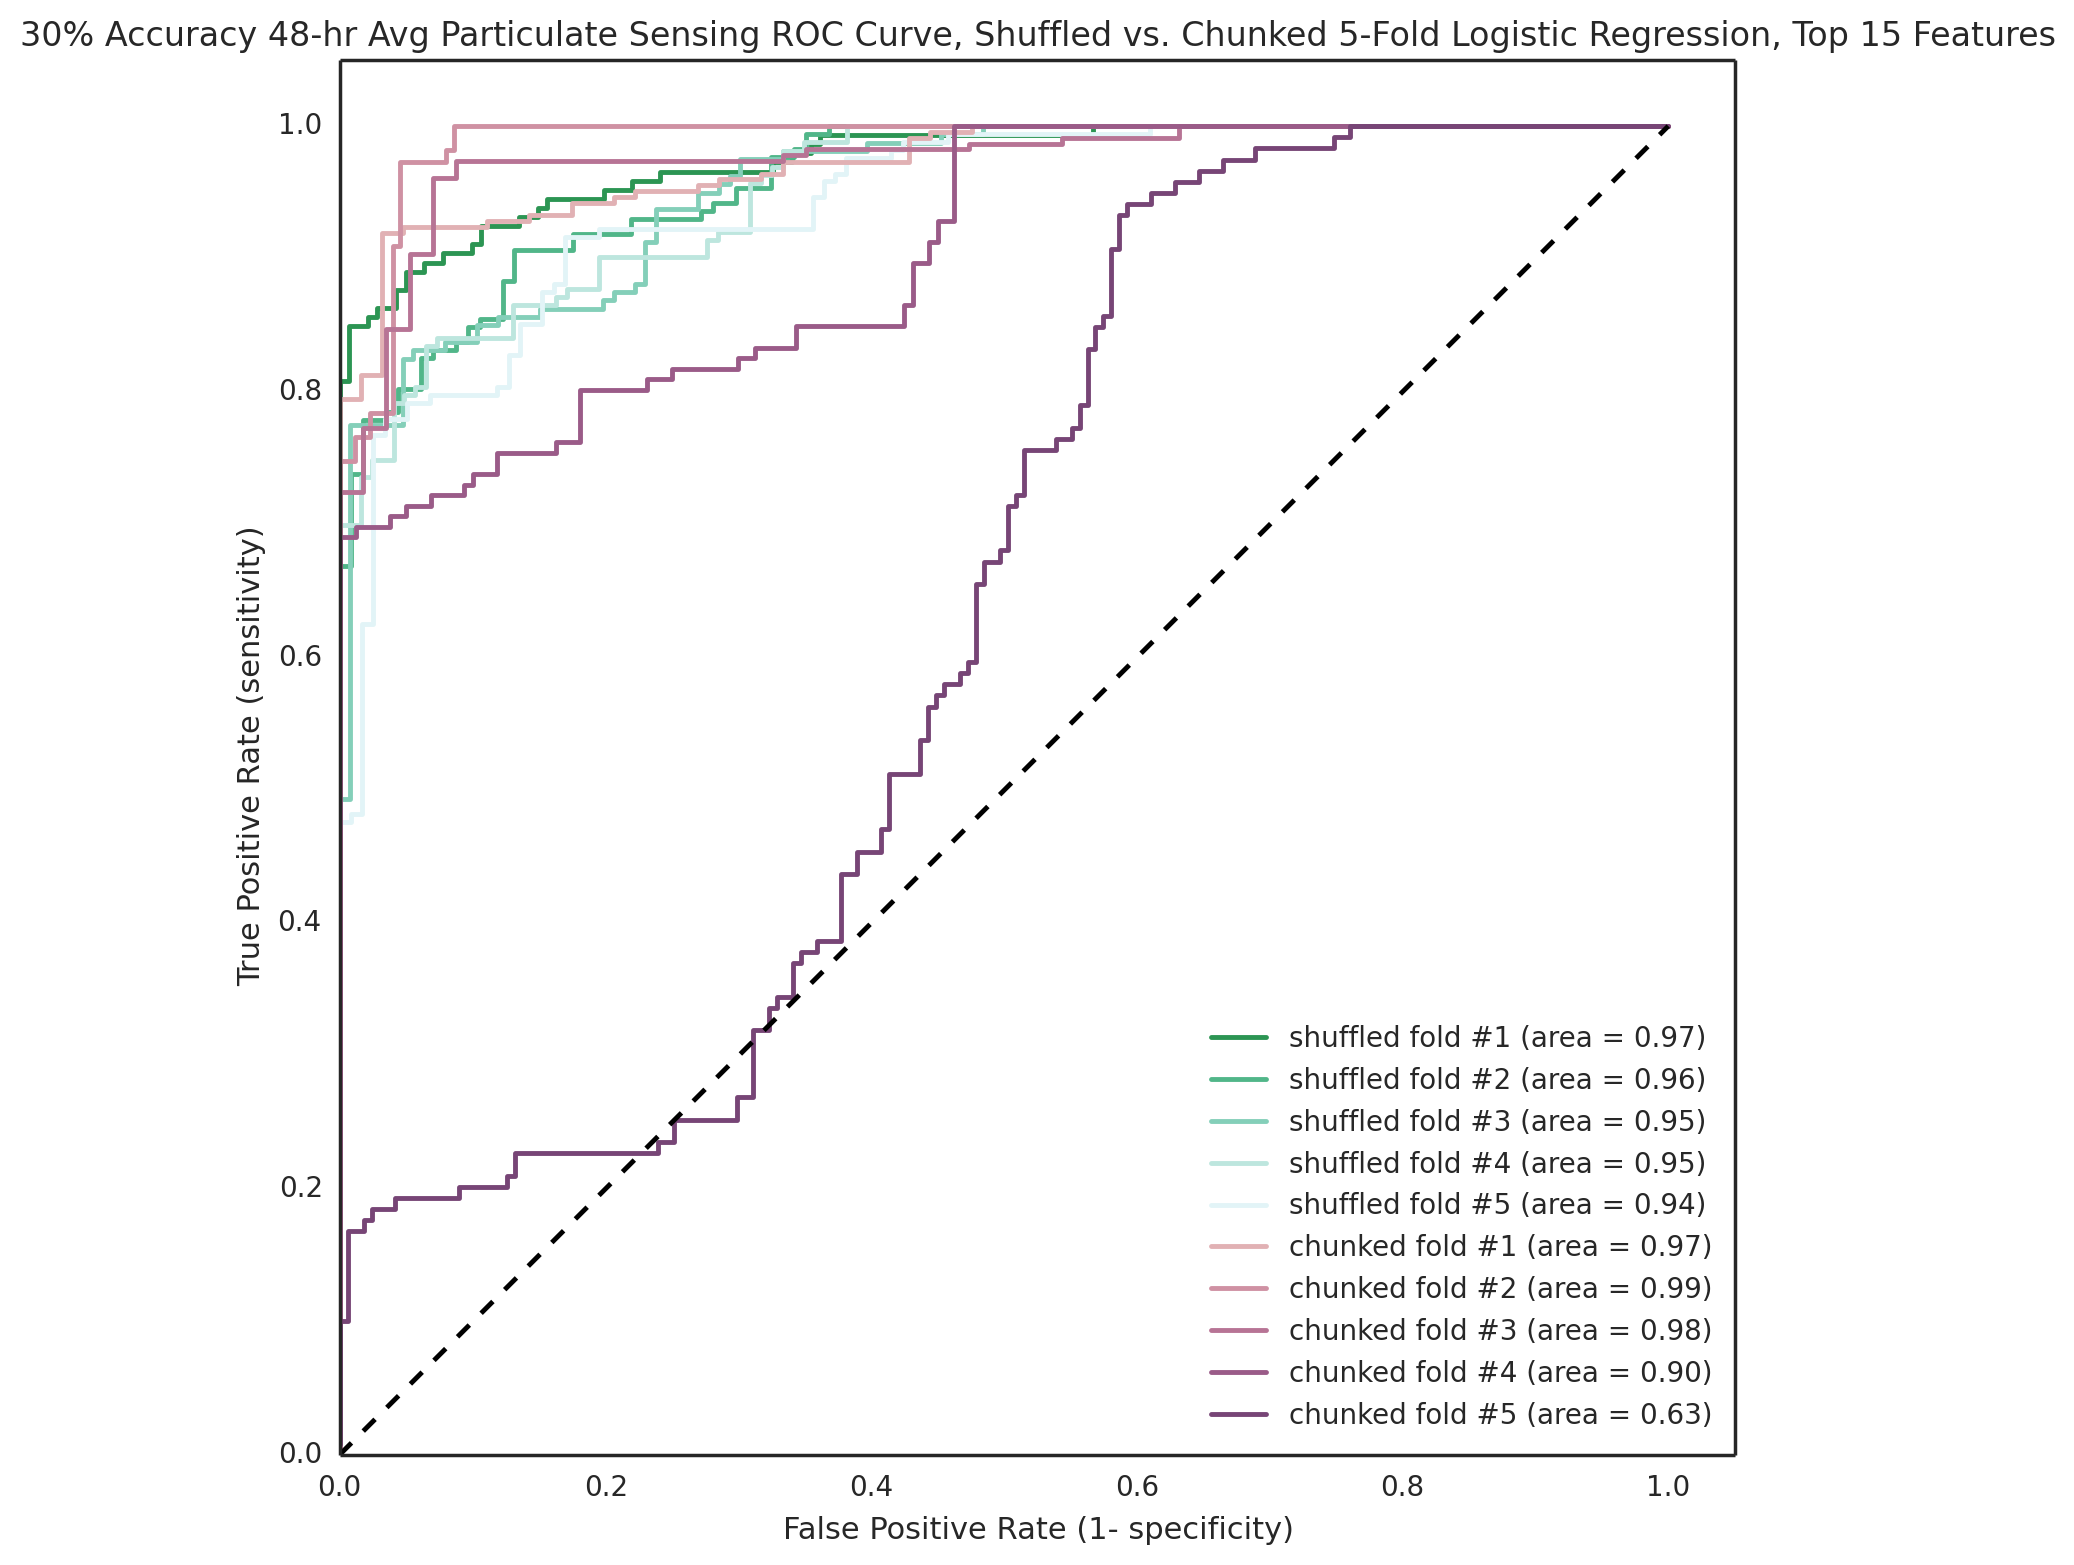
\includegraphics[width=\textwidth]{figs/sharp_48_avg_goals_30_roc_pruned_features}               
 	 \caption{48-hour Average Sharp Particulate ROC Using Top 15 Features}
  	\label{fig:sharp_48_avg_goals_30_roc_pruned_features}
\end{figure}

\begin{figure}[htb]
 	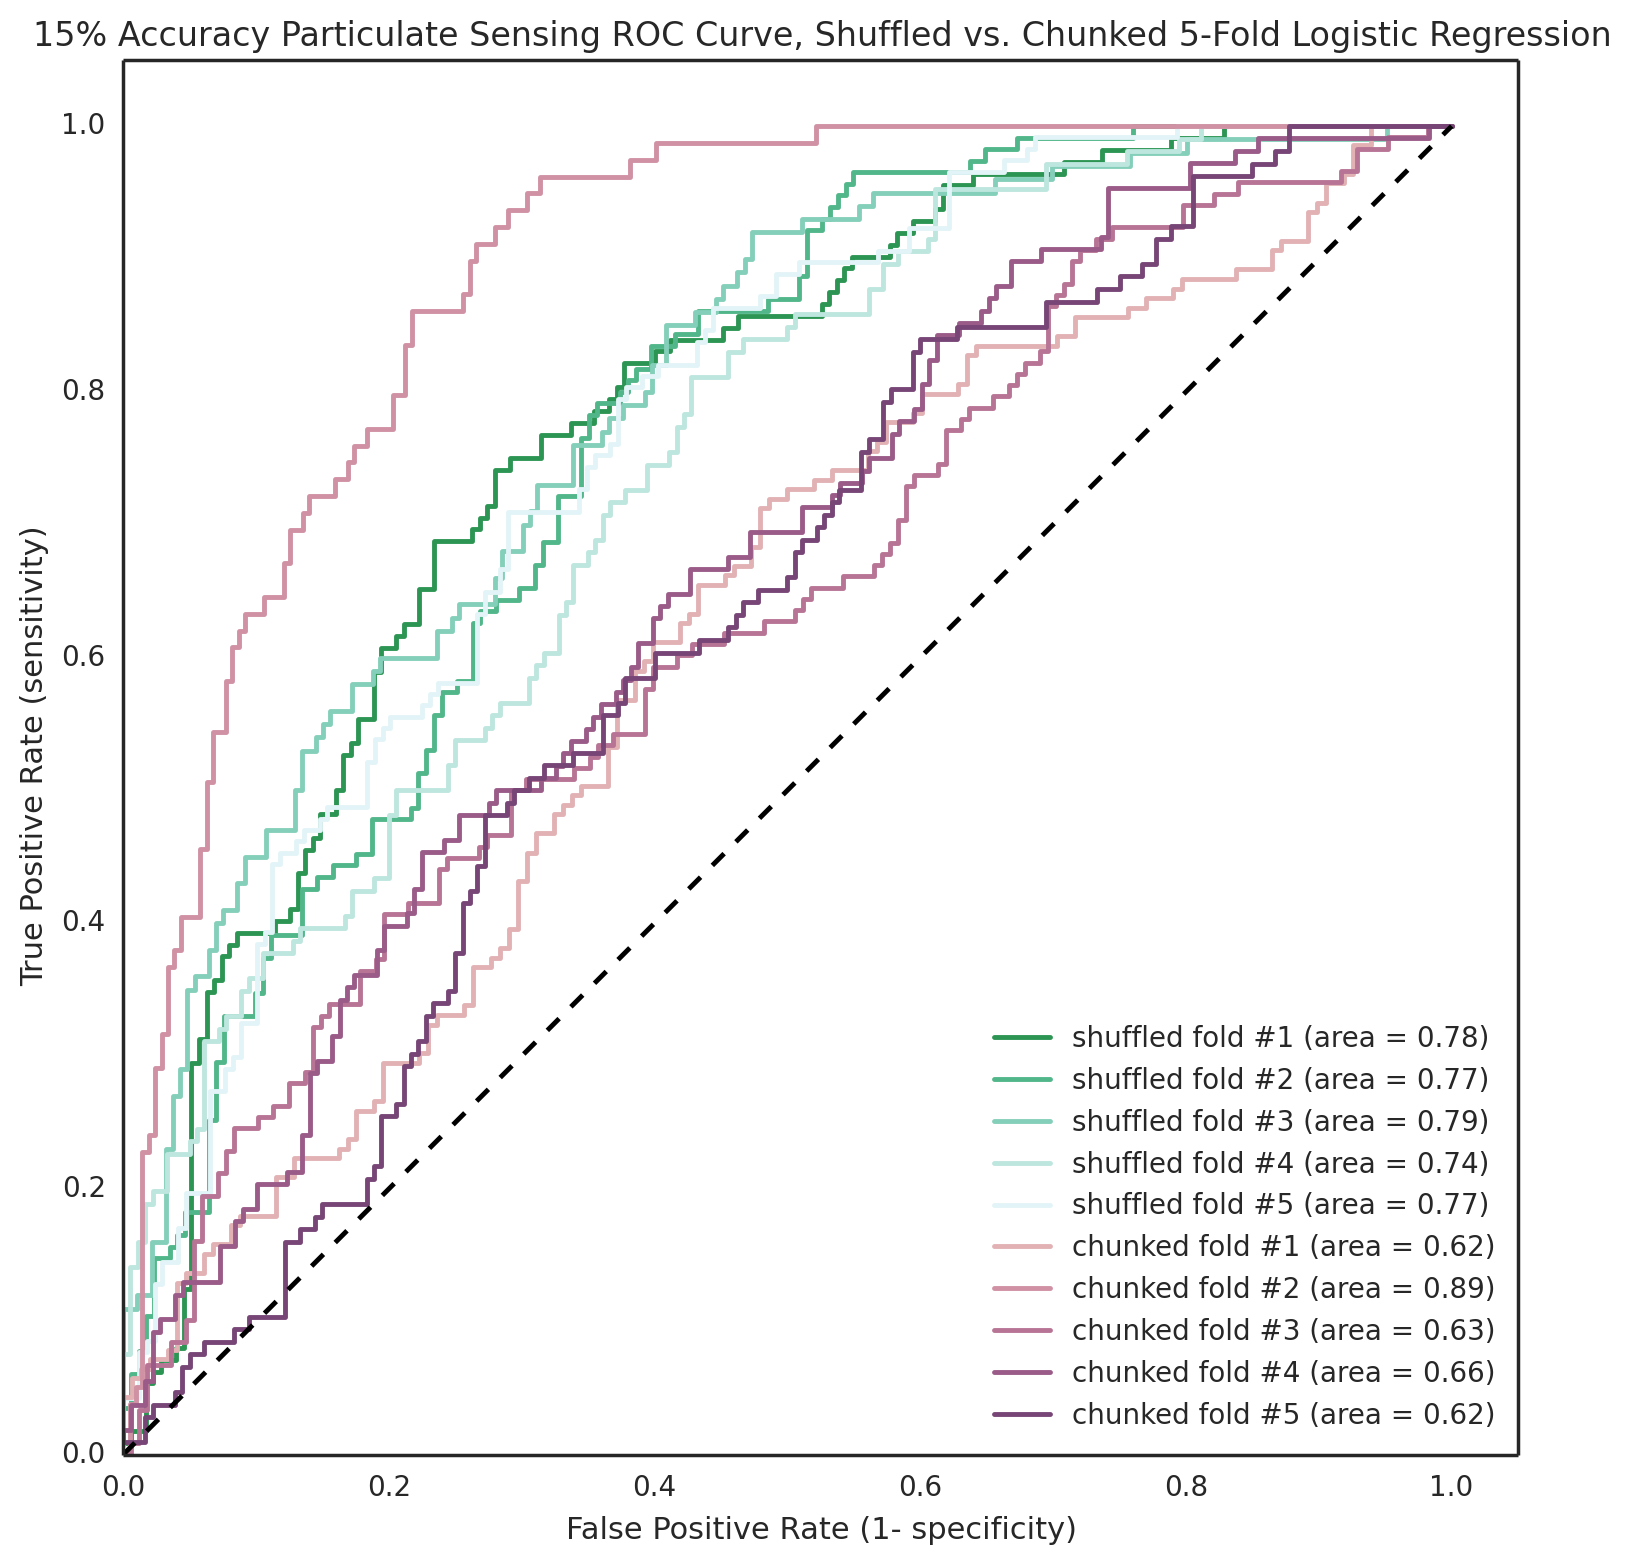
\includegraphics[width=\textwidth]{figs/sharp_goals_15_roc}               
 	 \caption{Reduced Tolerance Sharp Particulate ROC}
  	\label{fig:sharp_goals_15_roc}
\end{figure}

\begin{figure}[htb]
 	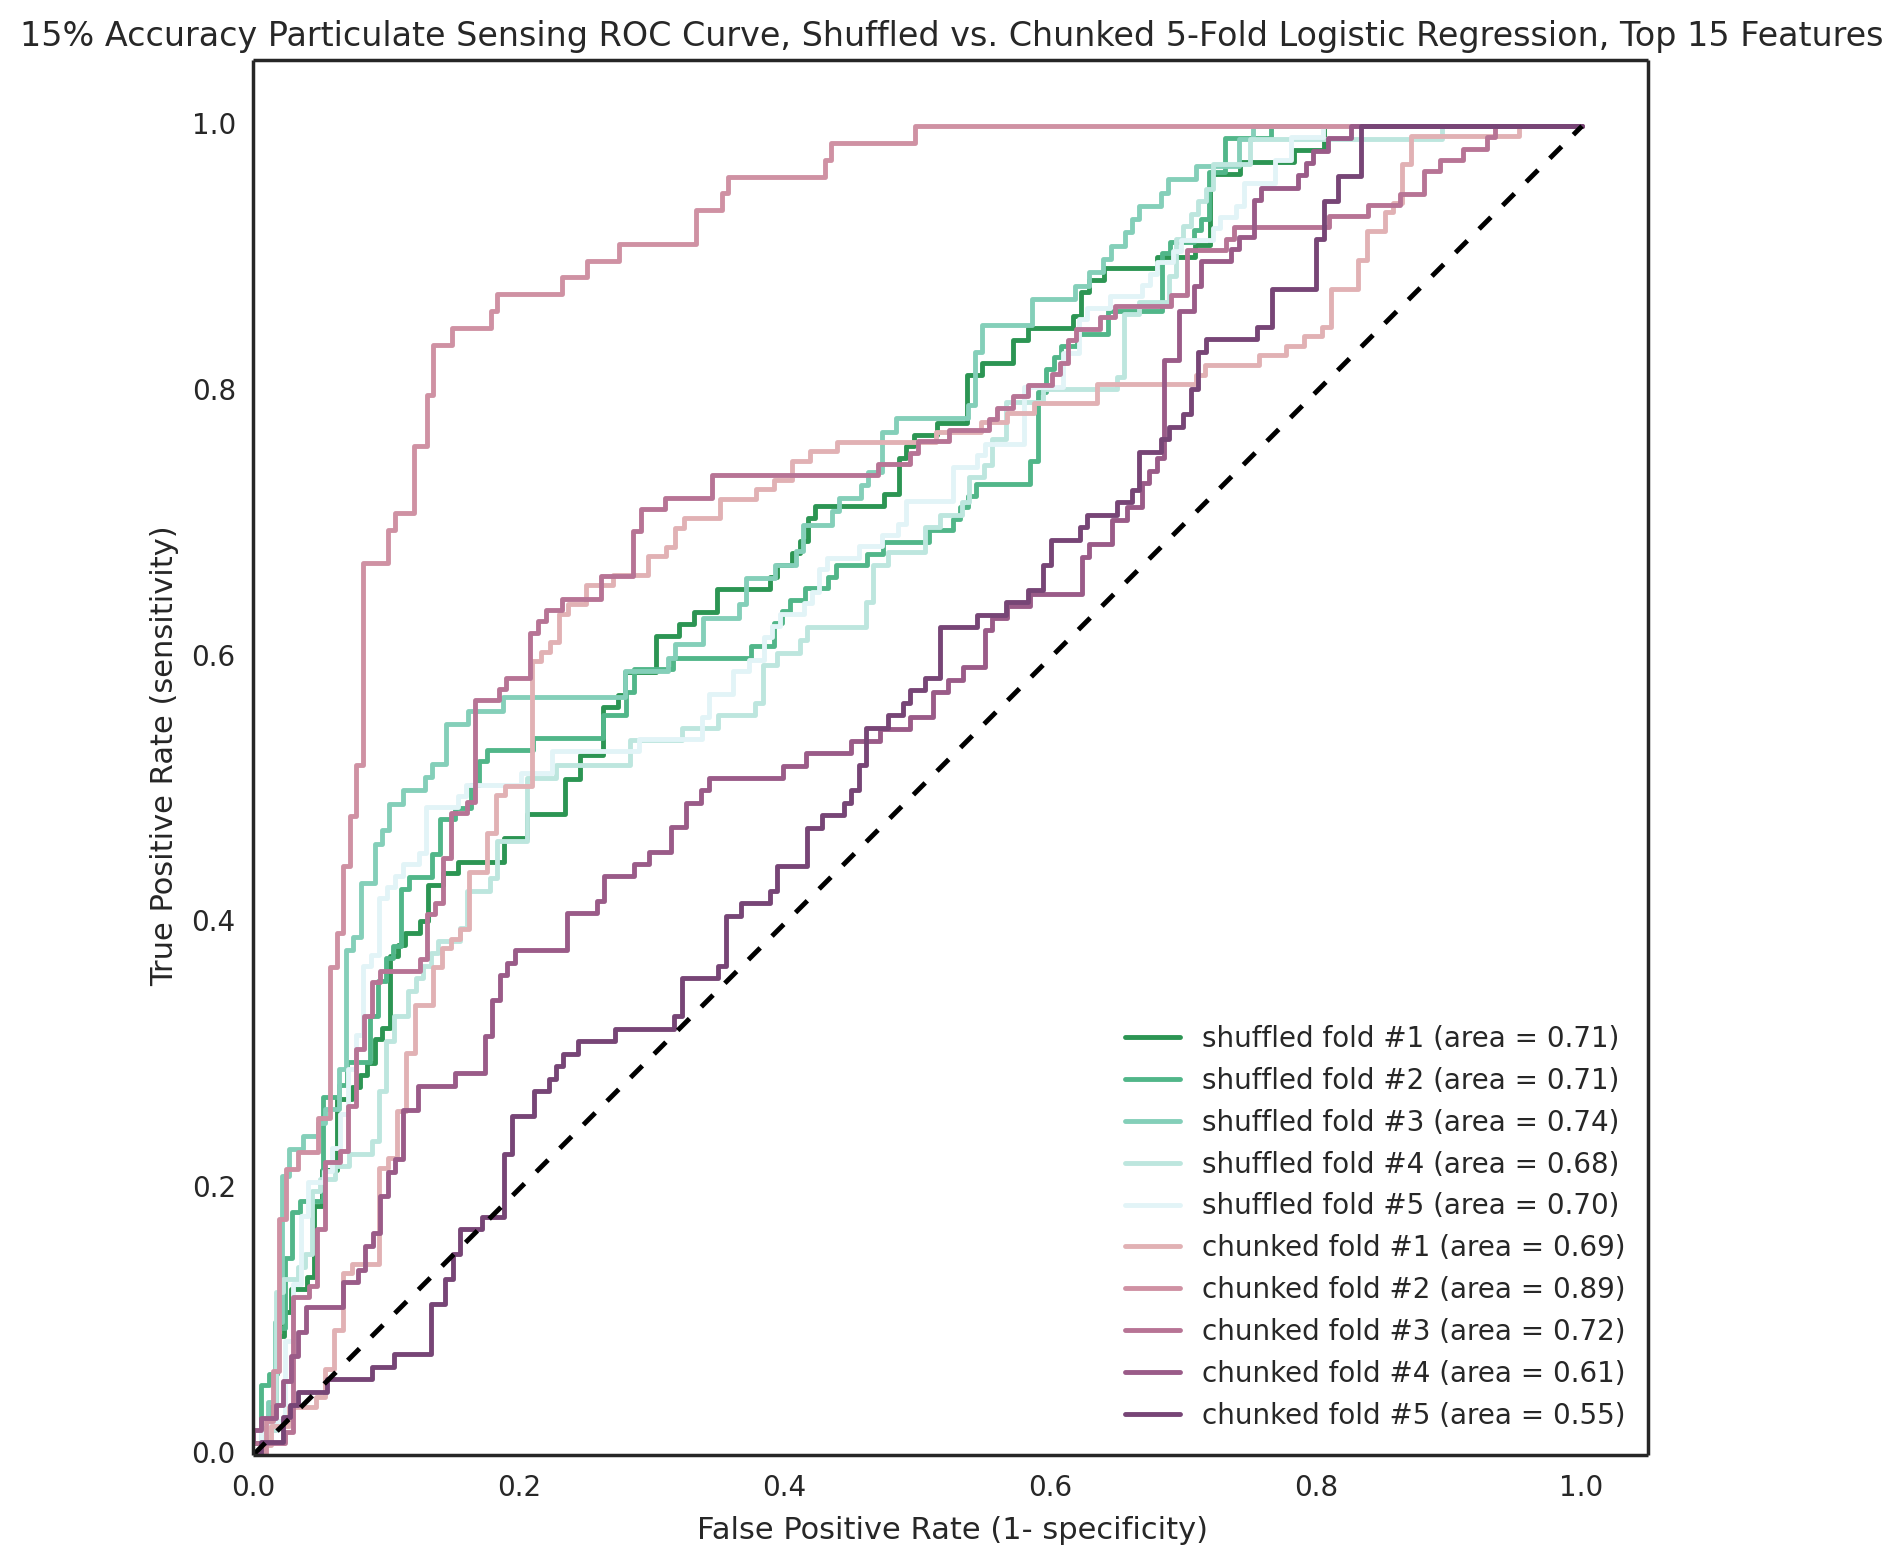
\includegraphics[width=\textwidth]{figs/sharp_goals_15_roc_pruned_features}               
 	 \caption{Reduced Tolerance Sharp Particulate ROC Using Top 15 Features}
  	\label{fig:sharp_goals_15_roc_pruned_features}
\end{figure}

\FloatBarrier
\section{AlphaSense CO}
\FloatBarrier

Following are additional plots from the AlphaSense CO test outlining the complete raw data and LMSE process, the accuracy with a tighter 7.5\% threshold, a visualization of the prediction accuracy and confidence, and the top 15 random forest selected features for both sensors tested.  Additionally, the ROC plots using just the top 15 features is included for both sensors.

\begin{figure}[htb]
 	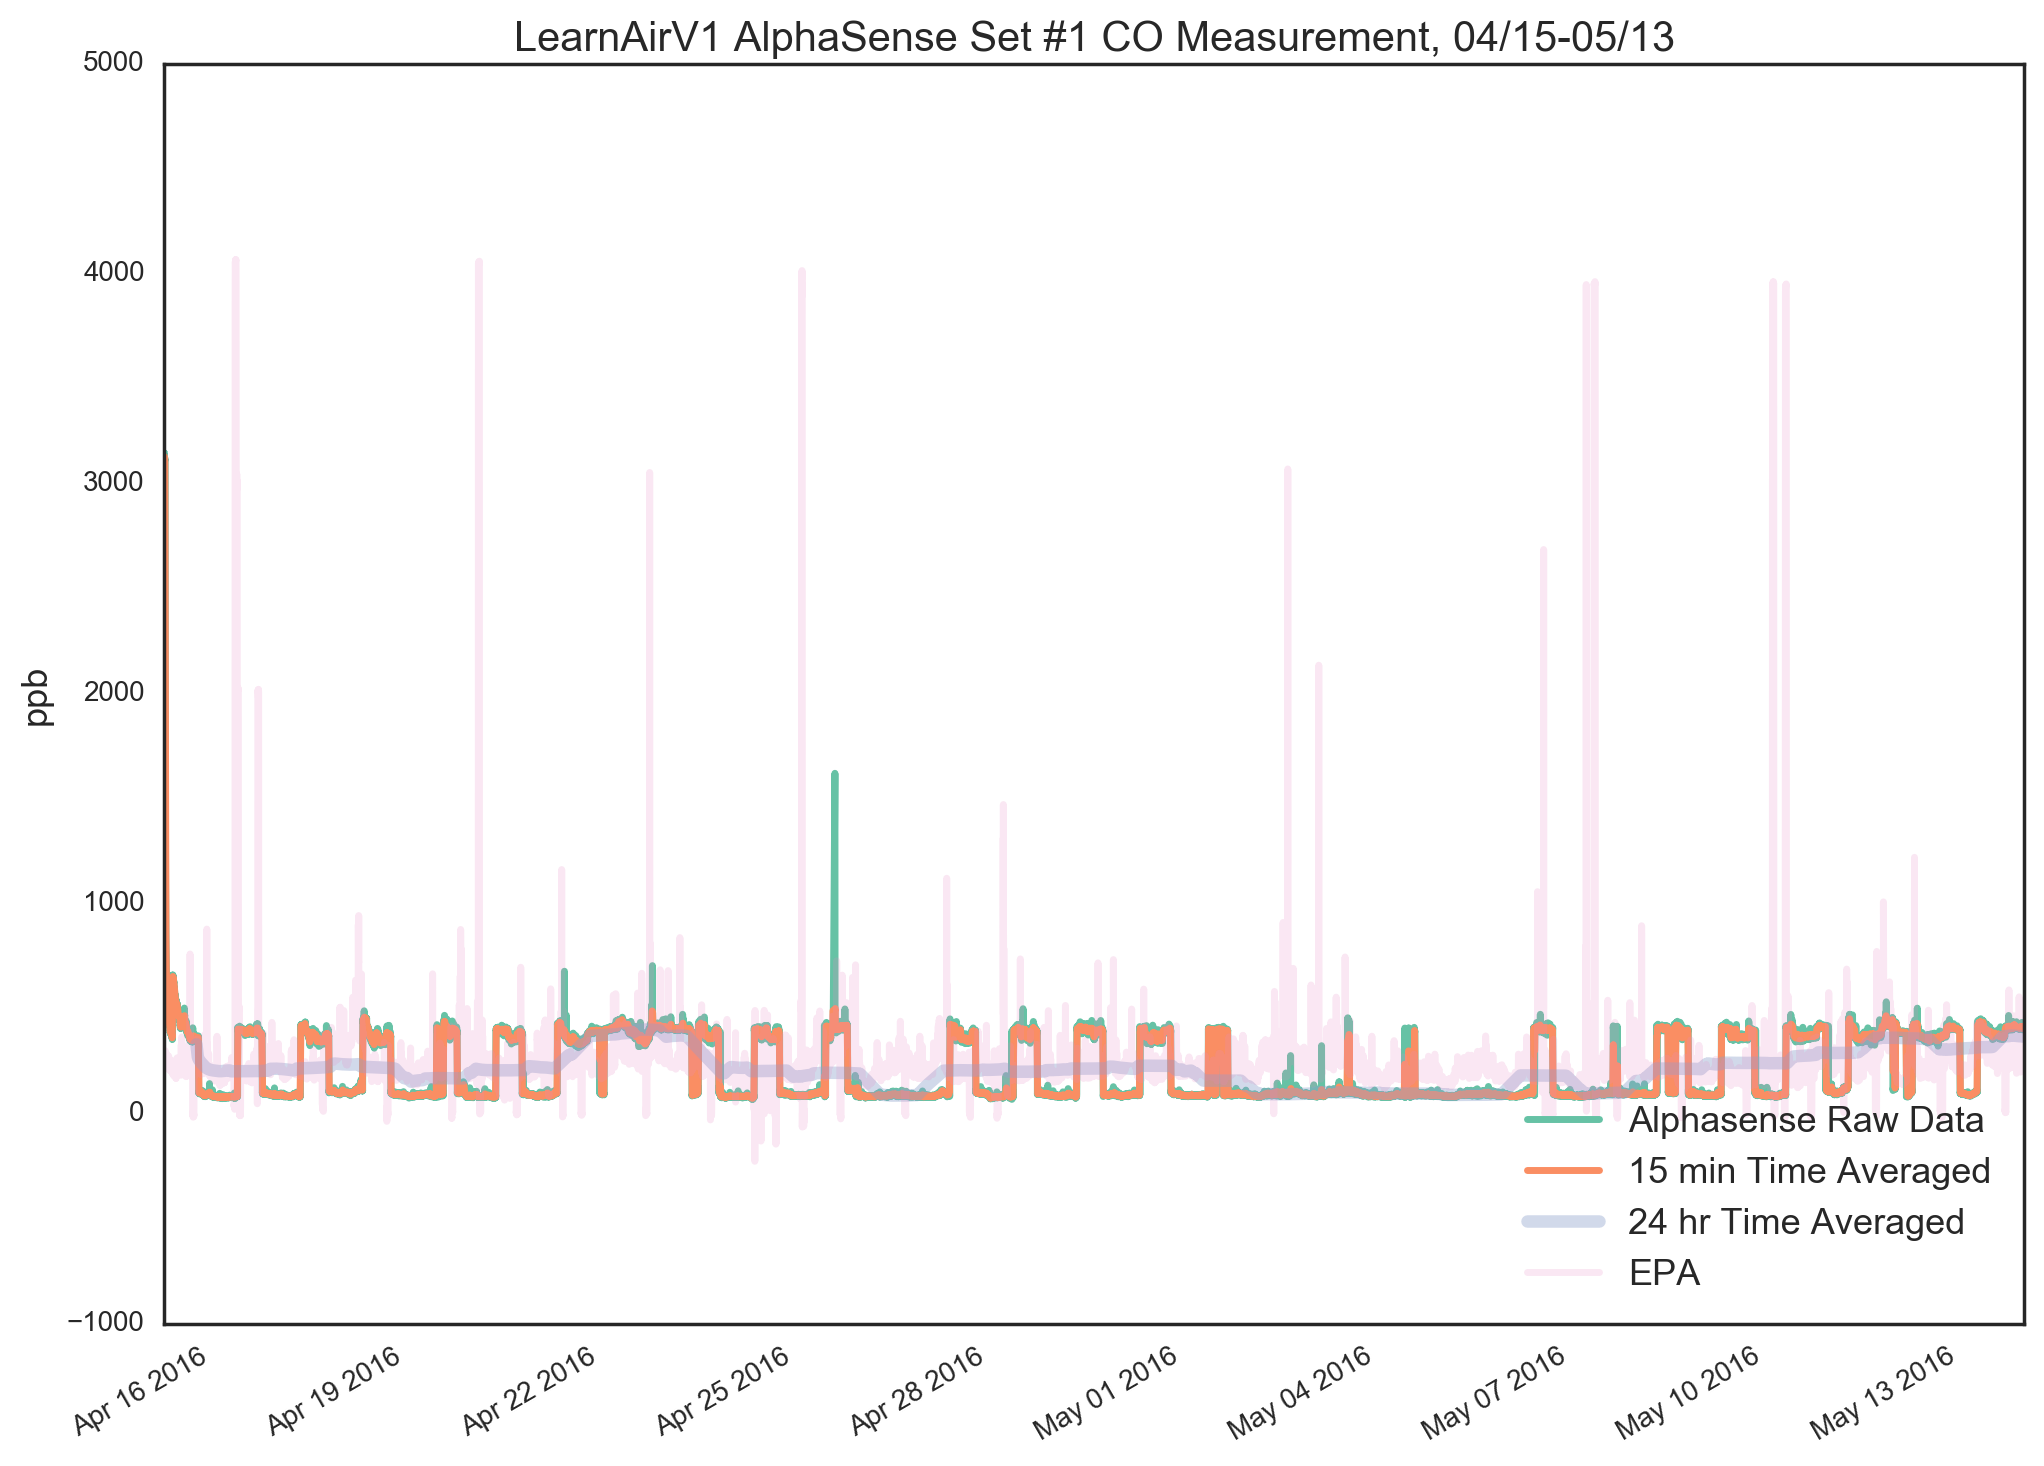
\includegraphics[width=\textwidth]{figs/as_co_raw}               
 	 \caption{AlphaSense CO Sensor #1 Raw Data}
  	\label{fig:as_co_raw}
\end{figure}

\begin{figure}[htb]
 	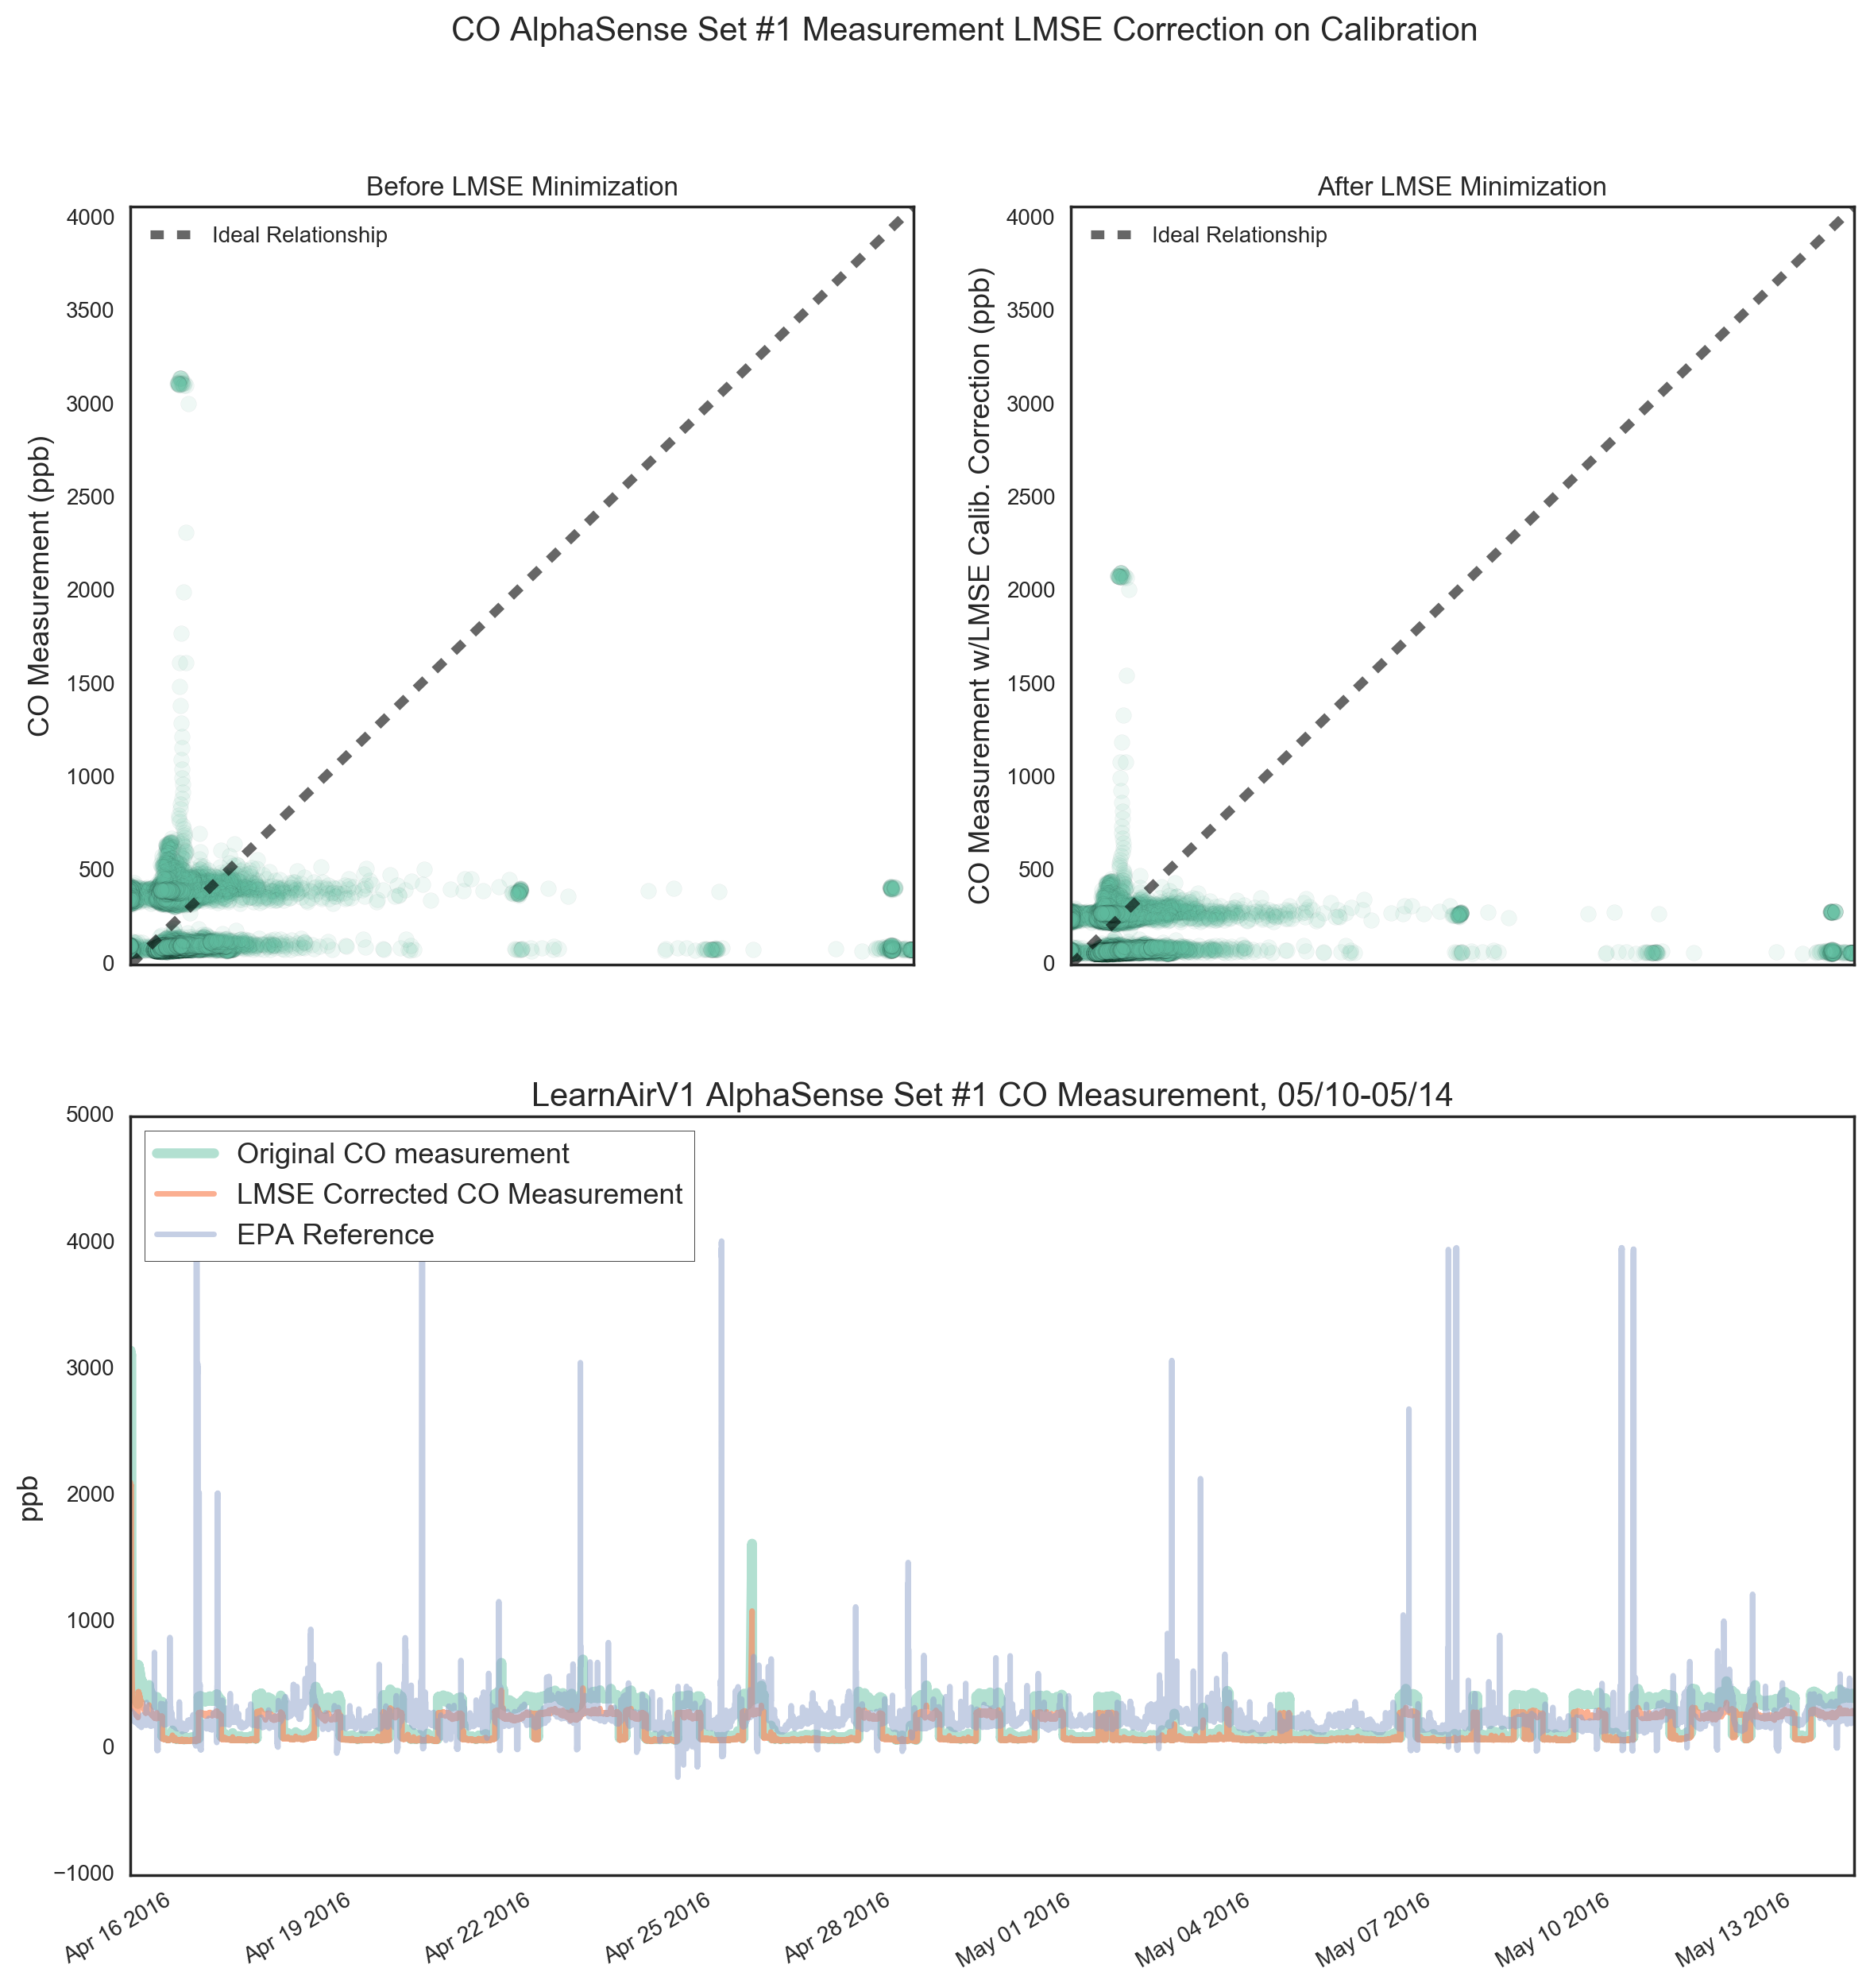
\includegraphics[width=\textwidth]{figs/as1_co_lmse}               
 	 \caption{AlphaSense CO Sensor #1 after LMSE Calibration}
  	\label{fig:as1_co_lmse}
\end{figure}

\begin{figure}[htb]
 	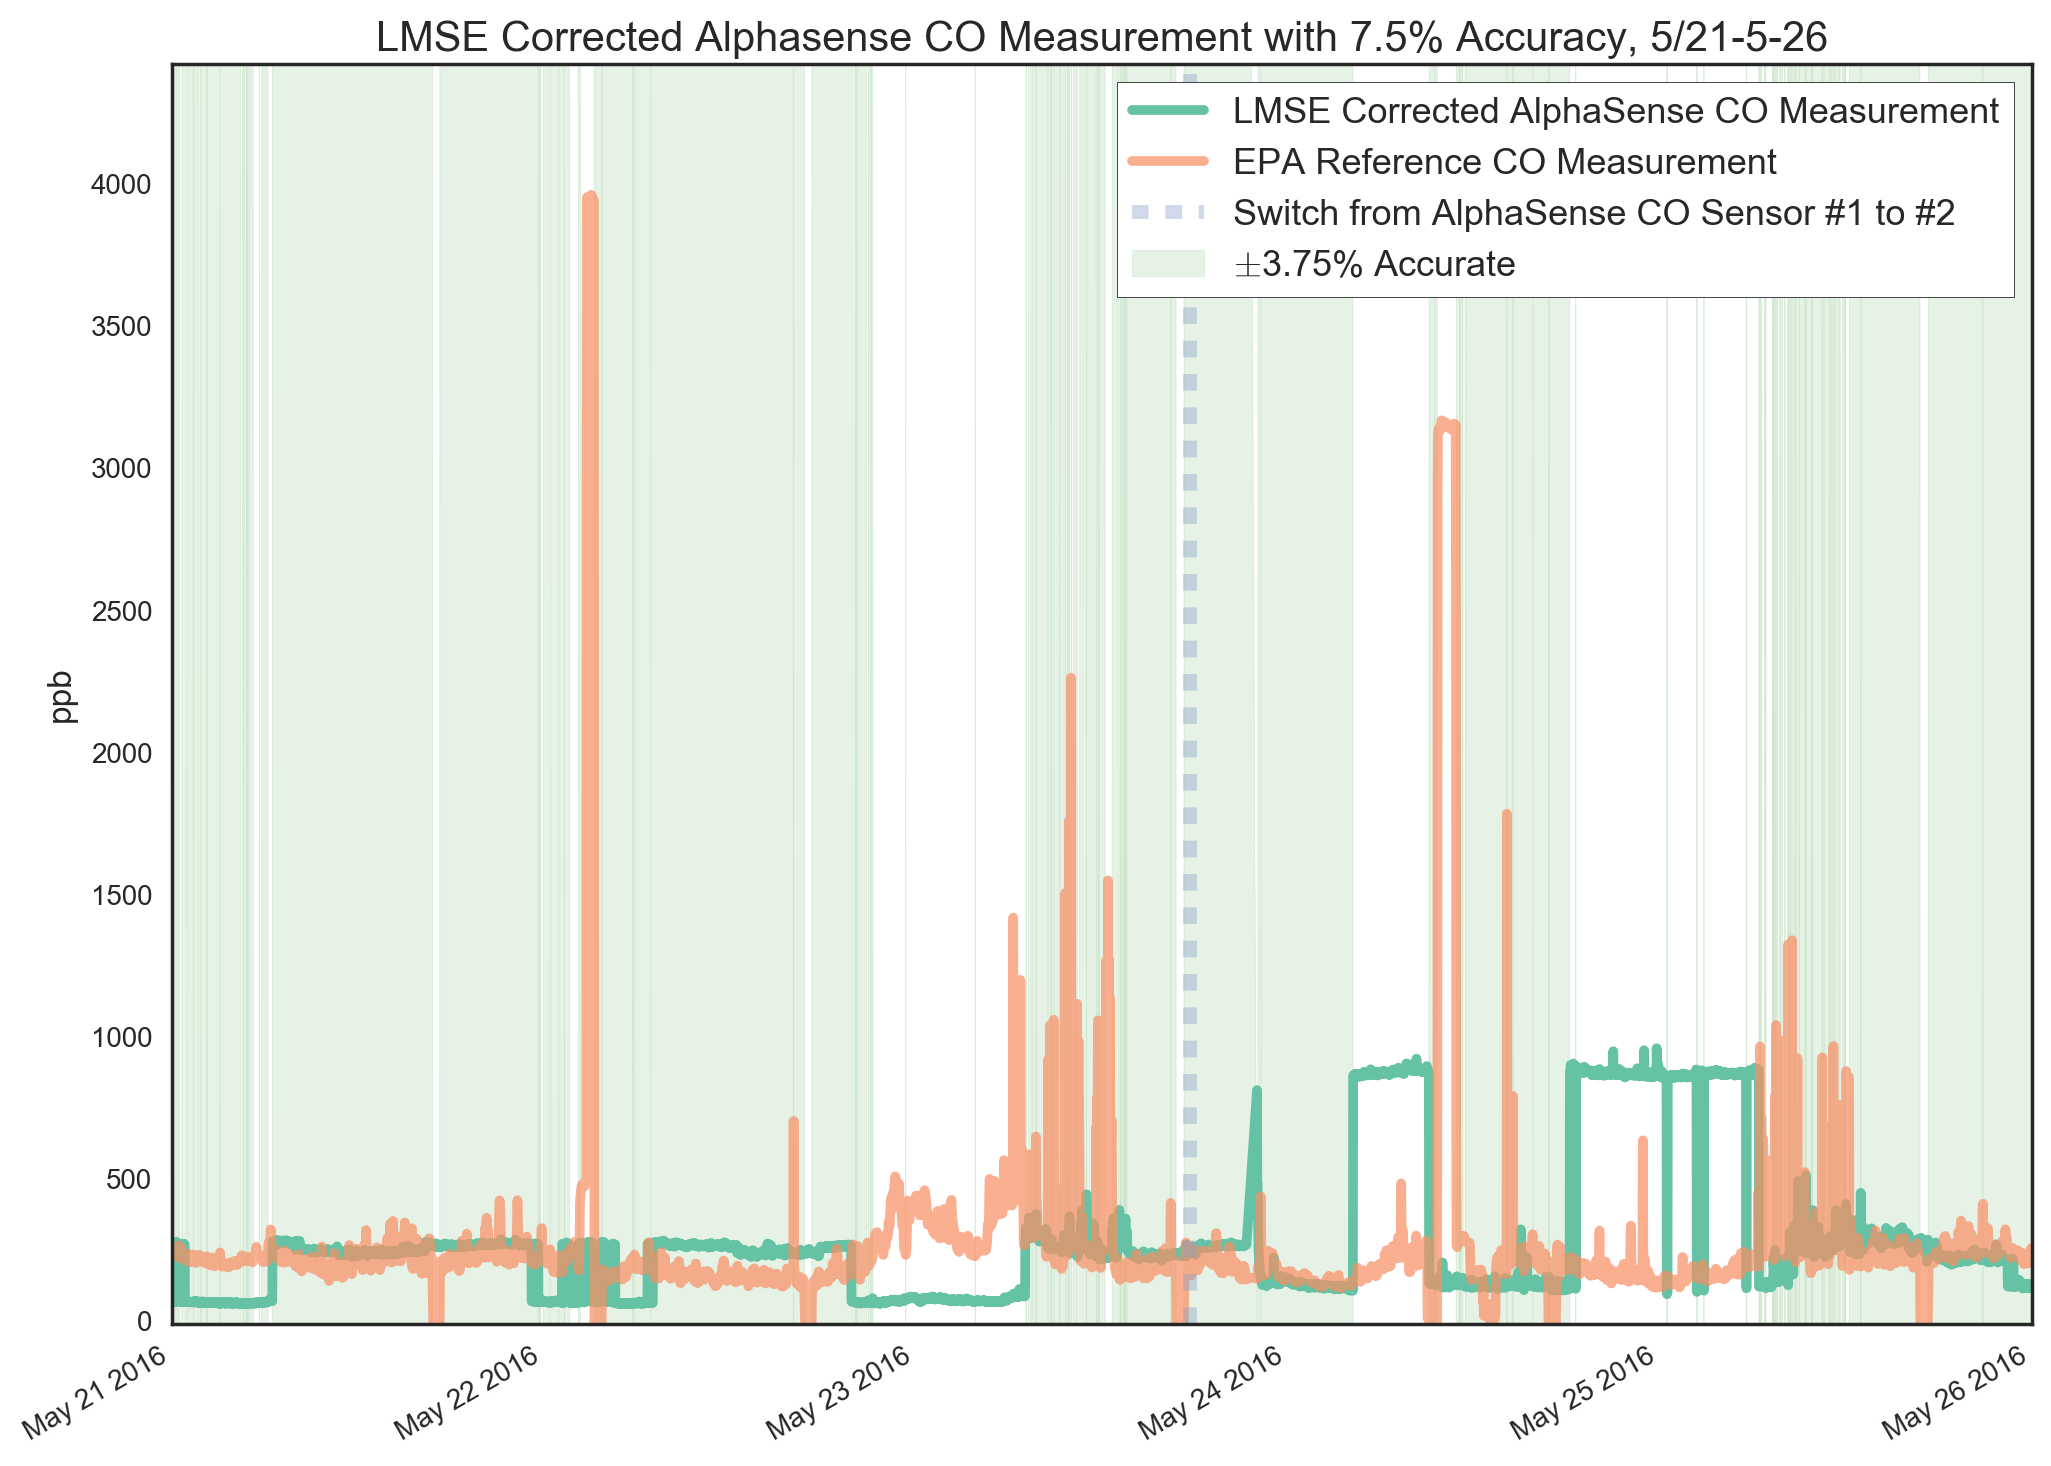
\includegraphics[width=\textwidth]{figs/as_co_with_7p5_accuracy_zoomed}               
 	 \caption{AlphaSense CO Sensor #1 and #2 with 7.5\% Accuracy Threshold}
  	\label{fig:as_co_with_7p5_accuracy_zoomed}
\end{figure}

\begin{figure}[htb]
 	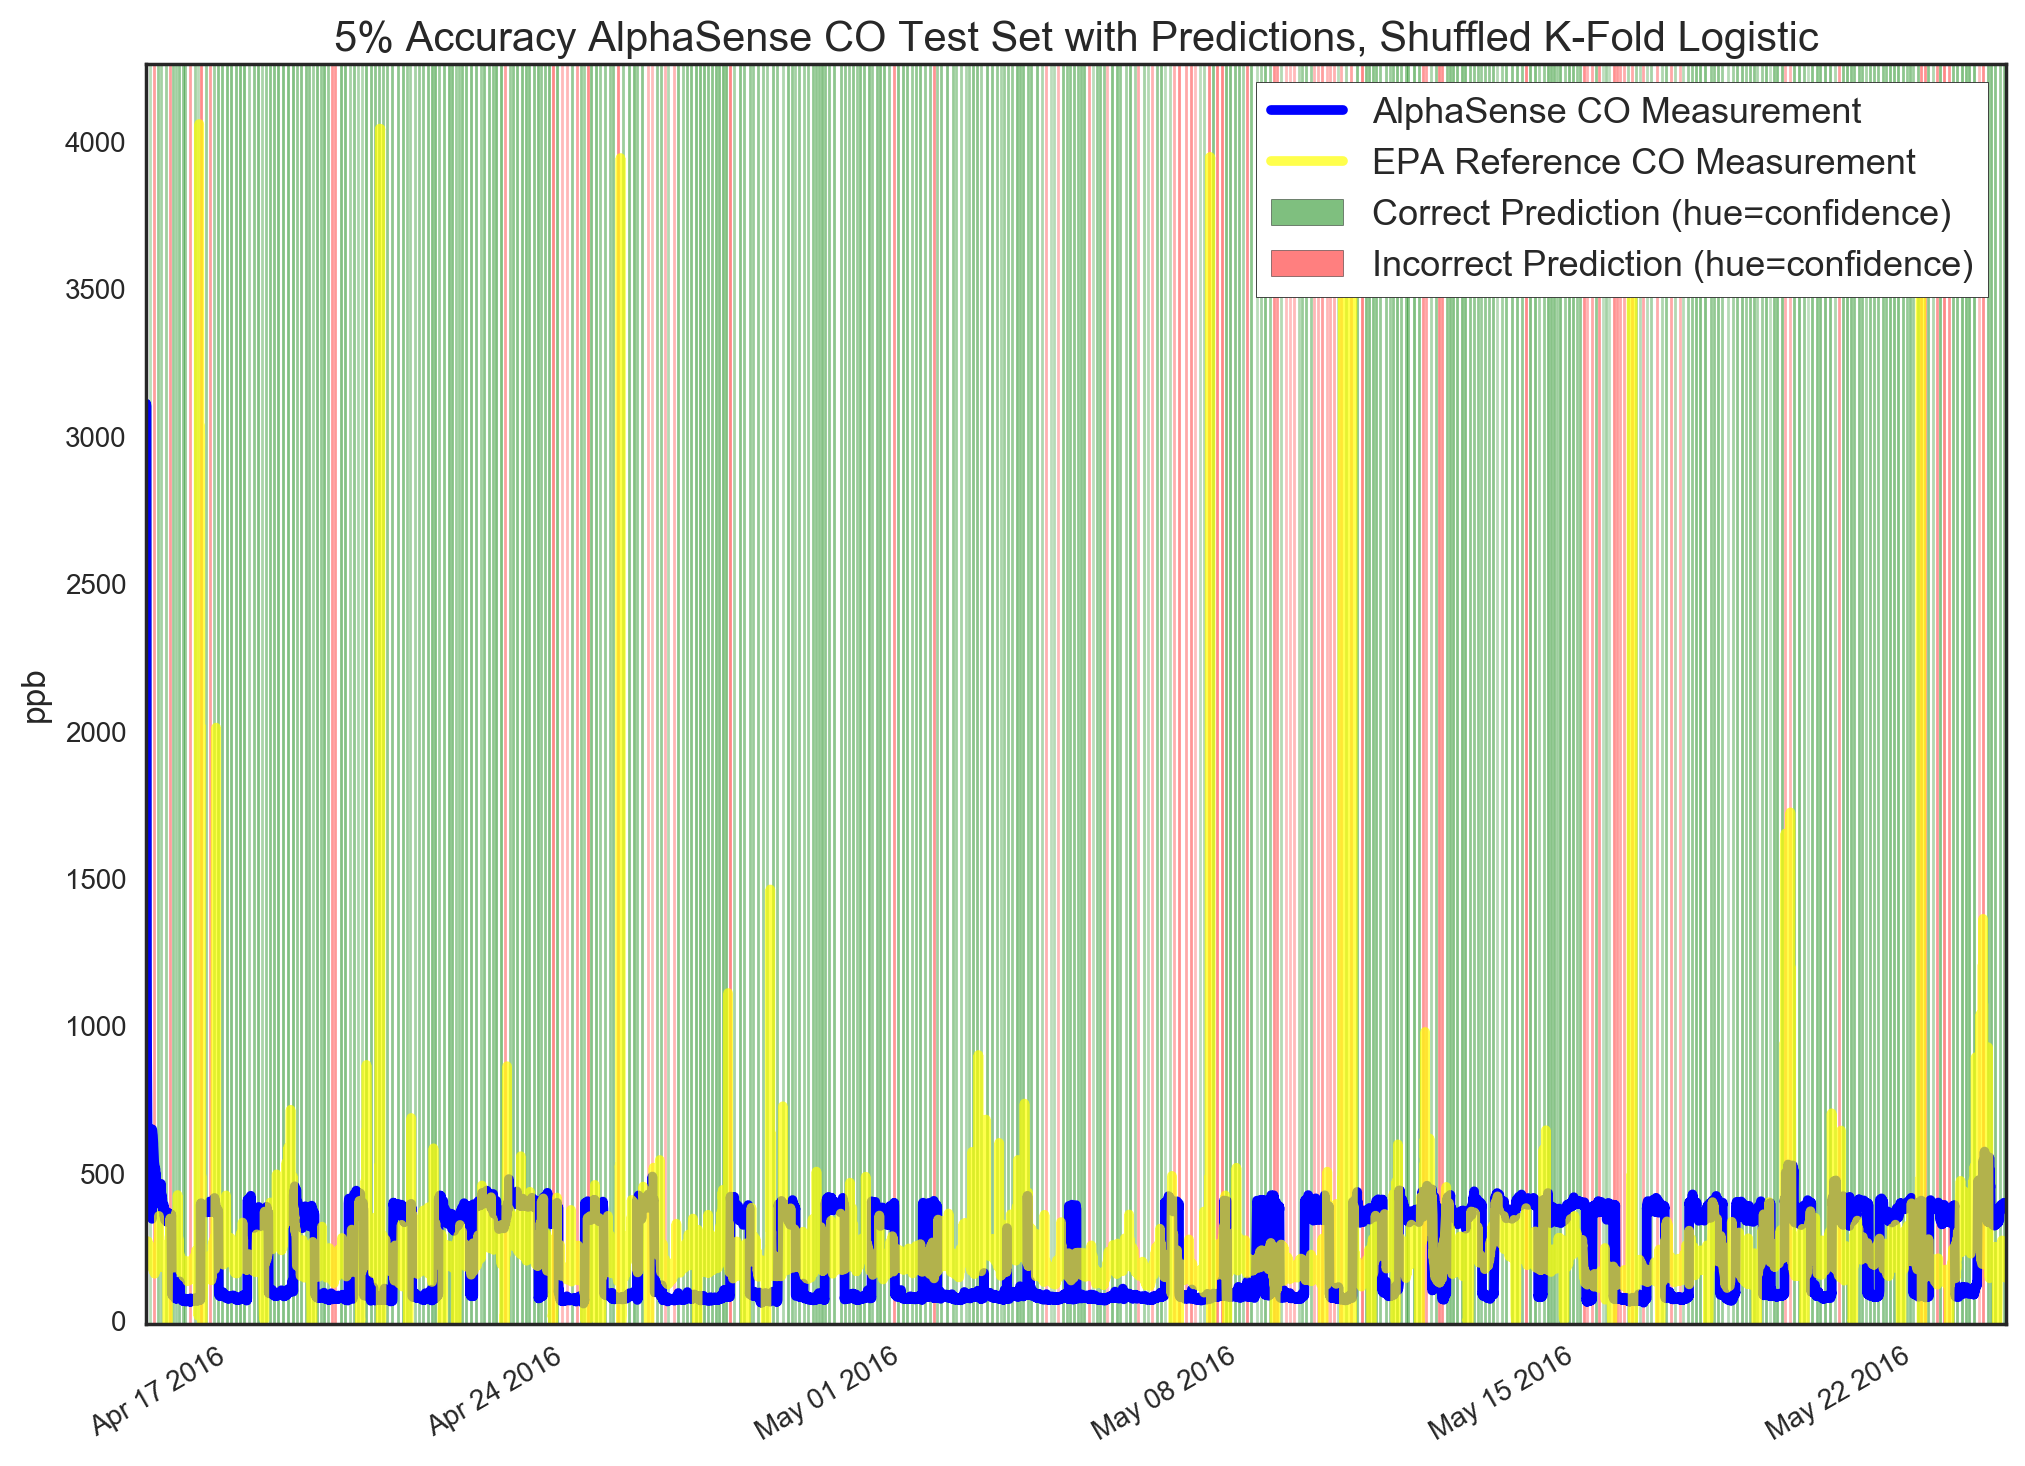
\includegraphics[width=\textwidth]{figs/as1_co_5_logistic_predictions}               
 	 \caption{AlphaSense CO Sensor #1 Prediction Accuracy}
  	\label{fig:as1_co_5_logistic_predictions}
\end{figure}

\begin{table}[]
\centering
\small
\begin{tabular}{lllllllll}
\\
\\
\toprule
Feature & Importance \\
\midrule
lmse\_calib\_as\_co & 0.0331983839664 \\
avg\_15\_lmse\_calib\_as\_co & 0.0331946346979 \\
avg\_15\_as\_co & 0.0322602817136 \\
as\_co & 0.0310204625161 \\
sck\_temperature & 0.0271023795431 \\
avg\_15\_as\_temperature & 0.0251288063362 \\
Temperature ( C RAW) & 0.024693128613 \\
avg\_60\_forecastio\_temperature_c & 0.0207050630804 \\
forecastio\_temperature\_c & 0.0192957142054 \\
as\_temperature & 0.018952457567 \\
avg\_60\_forecastio\_apparentTemperature & 0.017952895033 \\
alphaTemp & 0.0177934801727 \\
temp\_as\_box\_differential & 0.017581796276 \\
forecastio\_temperature & 0.0159096583245 \\
temp\_sck\_box\_differential & 0.0150463135619 \\
\bottomrule
\end{tabular}
\label{tab:as1_co_randomforest_features}
\caption{Top 15 Features from Random Forest for CO Sensor #1, used in Pruned Logistic Regression}
\end{table}



\begin{figure}[htb]
 	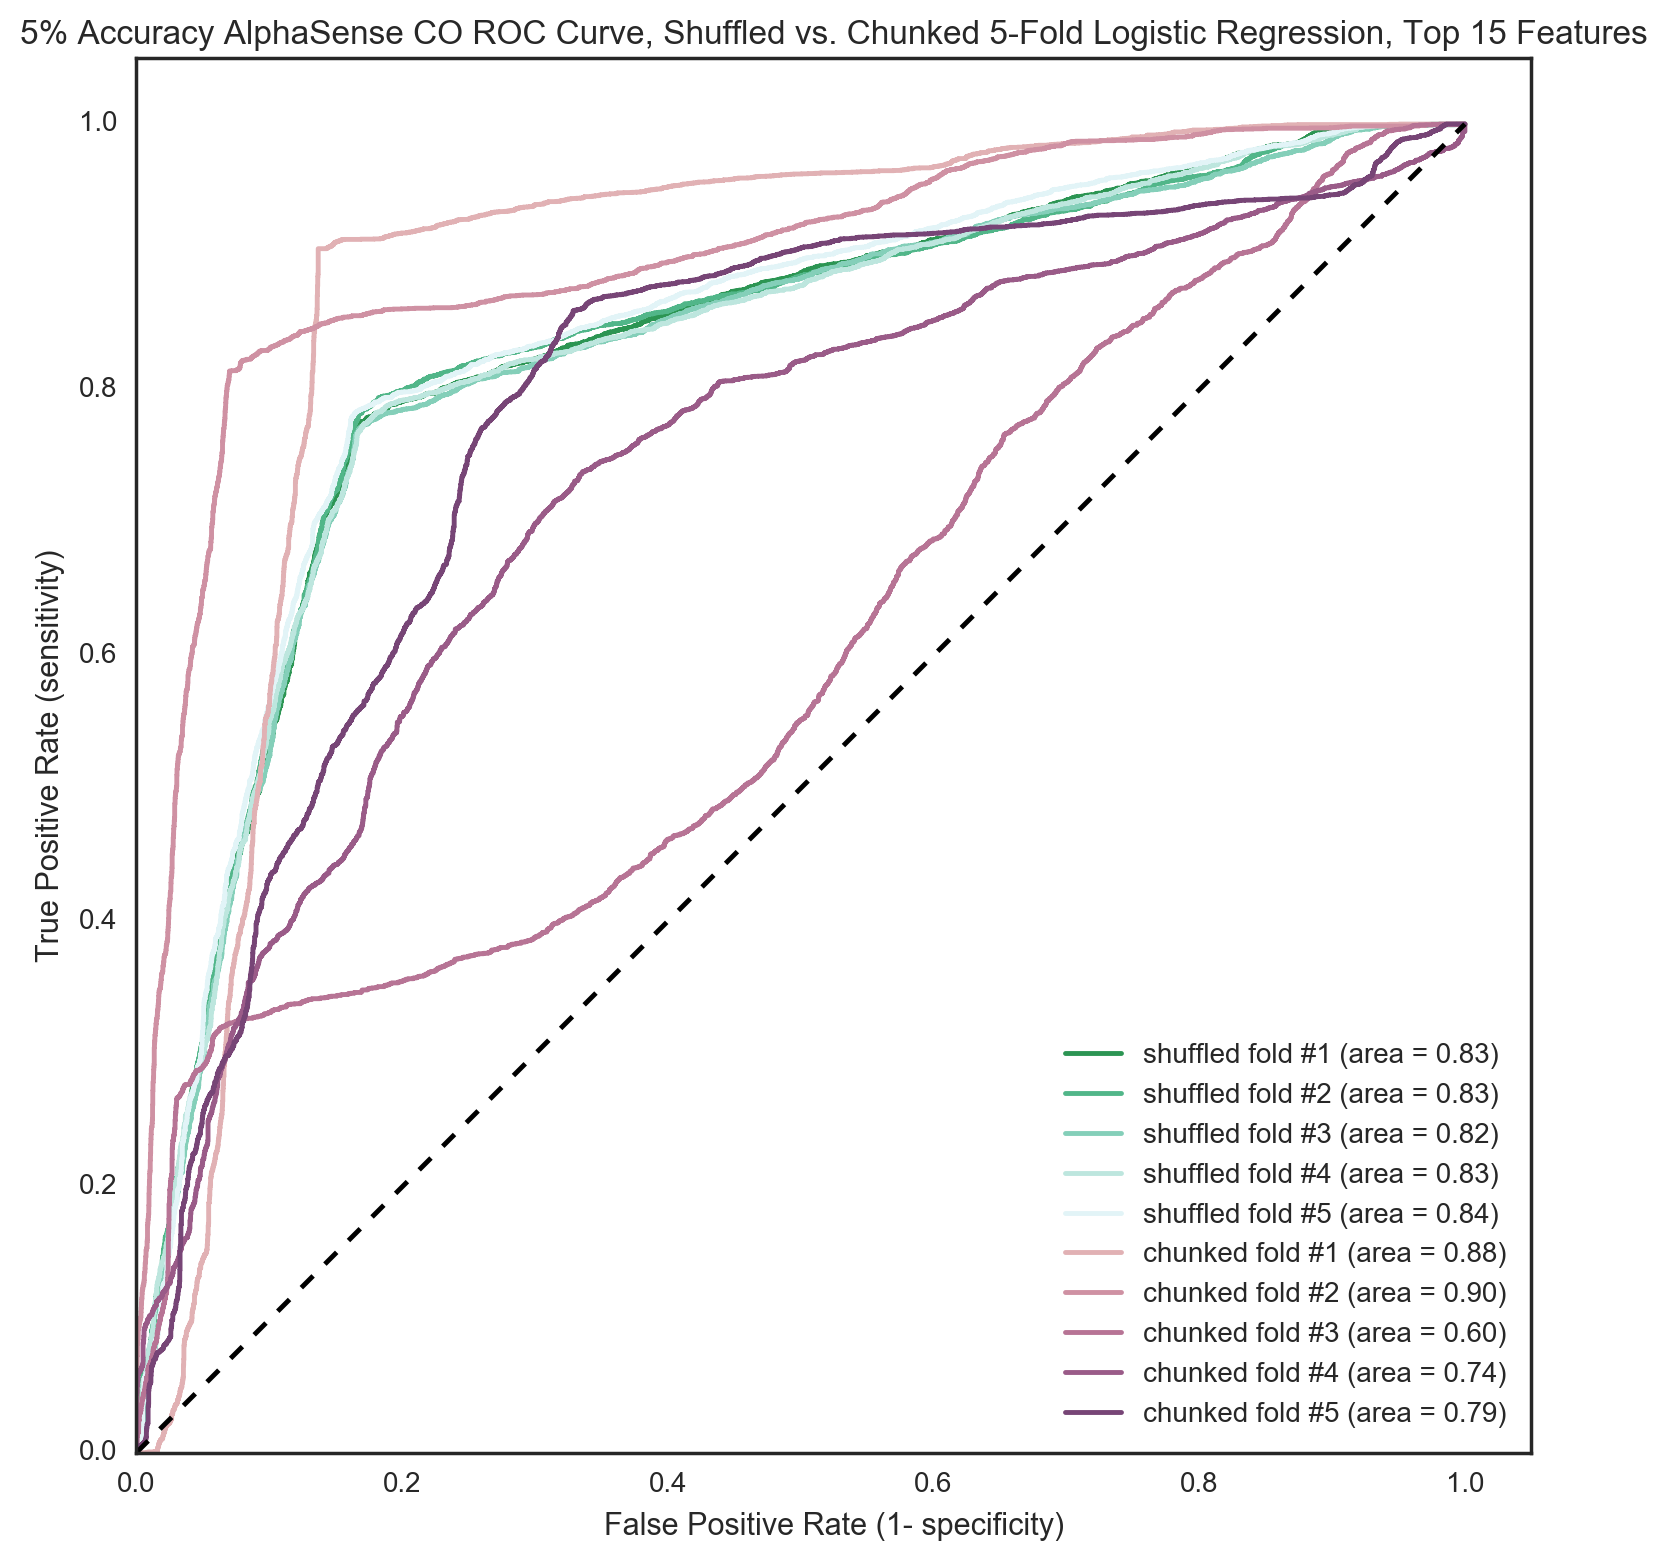
\includegraphics[width=\textwidth]{figs/as1_co_5_roc_pruned_features}               
 	 \caption{AlphaSense CO Sensor #1 ROC Using Top 15 Features}
  	\label{fig:as1_co_5_roc_pruned_features}
\end{figure}


\begin{table}[H]
\centering
\small
\begin{tabular}{lllllllll}
\\
\\
\toprule
Feature & Importance \\
\midrule
lmse\_calib\_as\_co & 0.0518584805682 \\
avg\_15\_lmse\_calib\_as\_co & 0.0404238890793 \\
avg\_720\_bkcarbon & 0.0222537733125 \\
avg\_60\_bkcarbon & 0.0216045744972 \\
avg\_1440\_bkcarbon & 0.0198813295966 \\
as\_o3 & 0.0198510401658 \\
lmse\_as\_no2 & 0.0197364055605 \\
avg\_10\_as\_o3 & 0.0196965727088 \\
bkcarbon & 0.0194862747741 \\
as\_no2 & 0.0192353467551 \\
avg\_15\_lmse\_as\_no2 & 0.0180978893662 \\
lmse\_avg\_15\_as\_no2 & 0.0172526534474 \\
avg\_15\_as\_no2 & 0.0162905415767 \\
avg\_15\_as\_co & 0.0158810645781 \\
as\_co & 0.0158442759727 \\
\bottomrule
\end{tabular}
\label{tab:as2_co_randomforest_features}
\caption{Top 15 Features from Random Forest for CO Sensor #2, used in Pruned Logistic Regression}
\end{table}


\begin{figure}[htb]
 	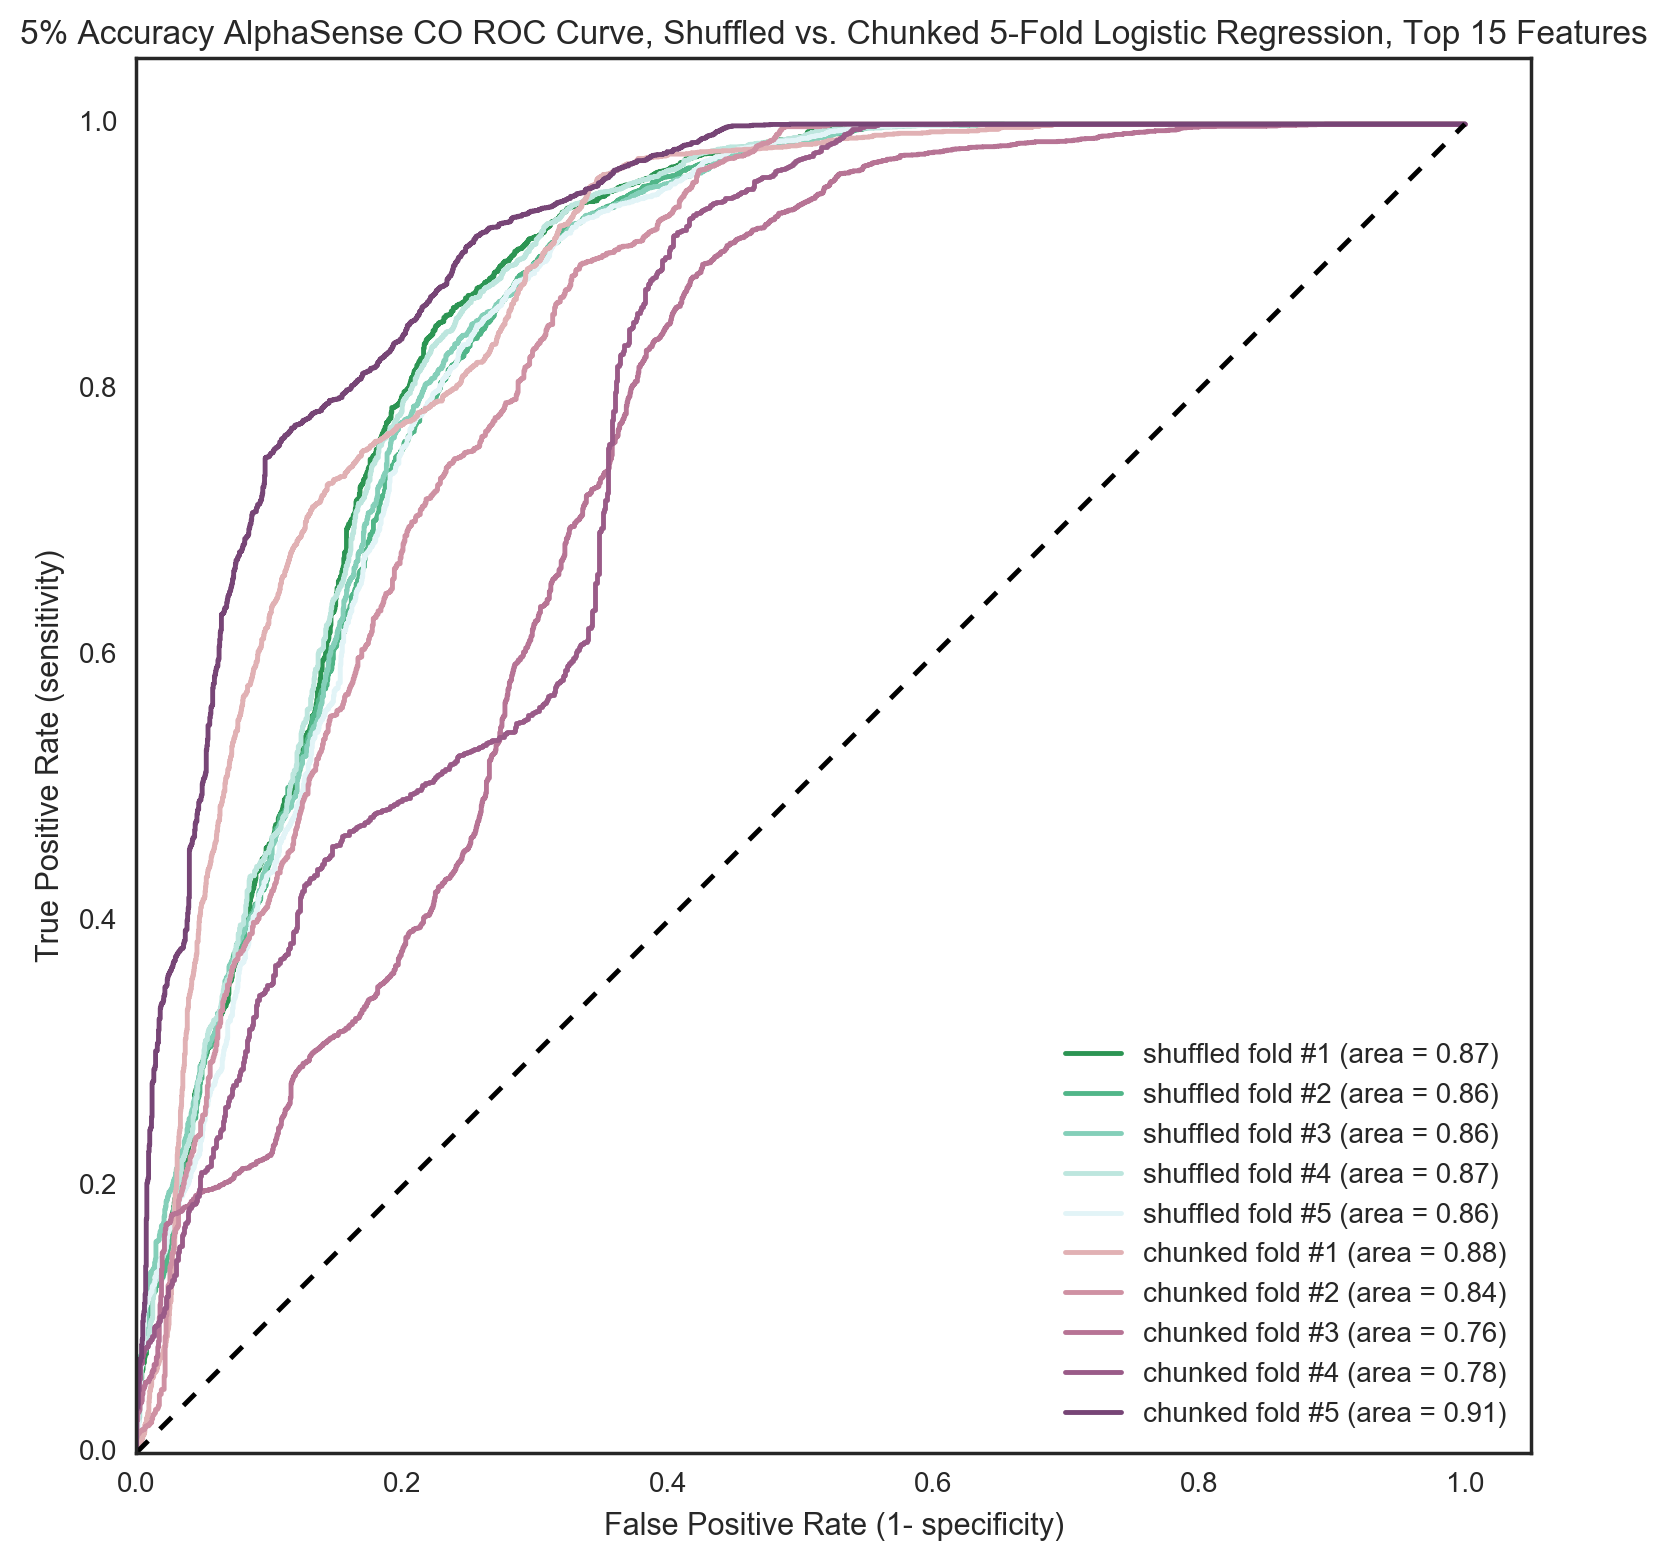
\includegraphics[width=\textwidth]{figs/as2_co_5_roc_pruned_features}               
 	 \caption{AlphaSense CO Sensor #2 ROC Using Top 15 Features}
  	\label{fig:as2_o3_7p5_roc_pruned_features}
\end{figure}

\begin{figure}[htb]
 	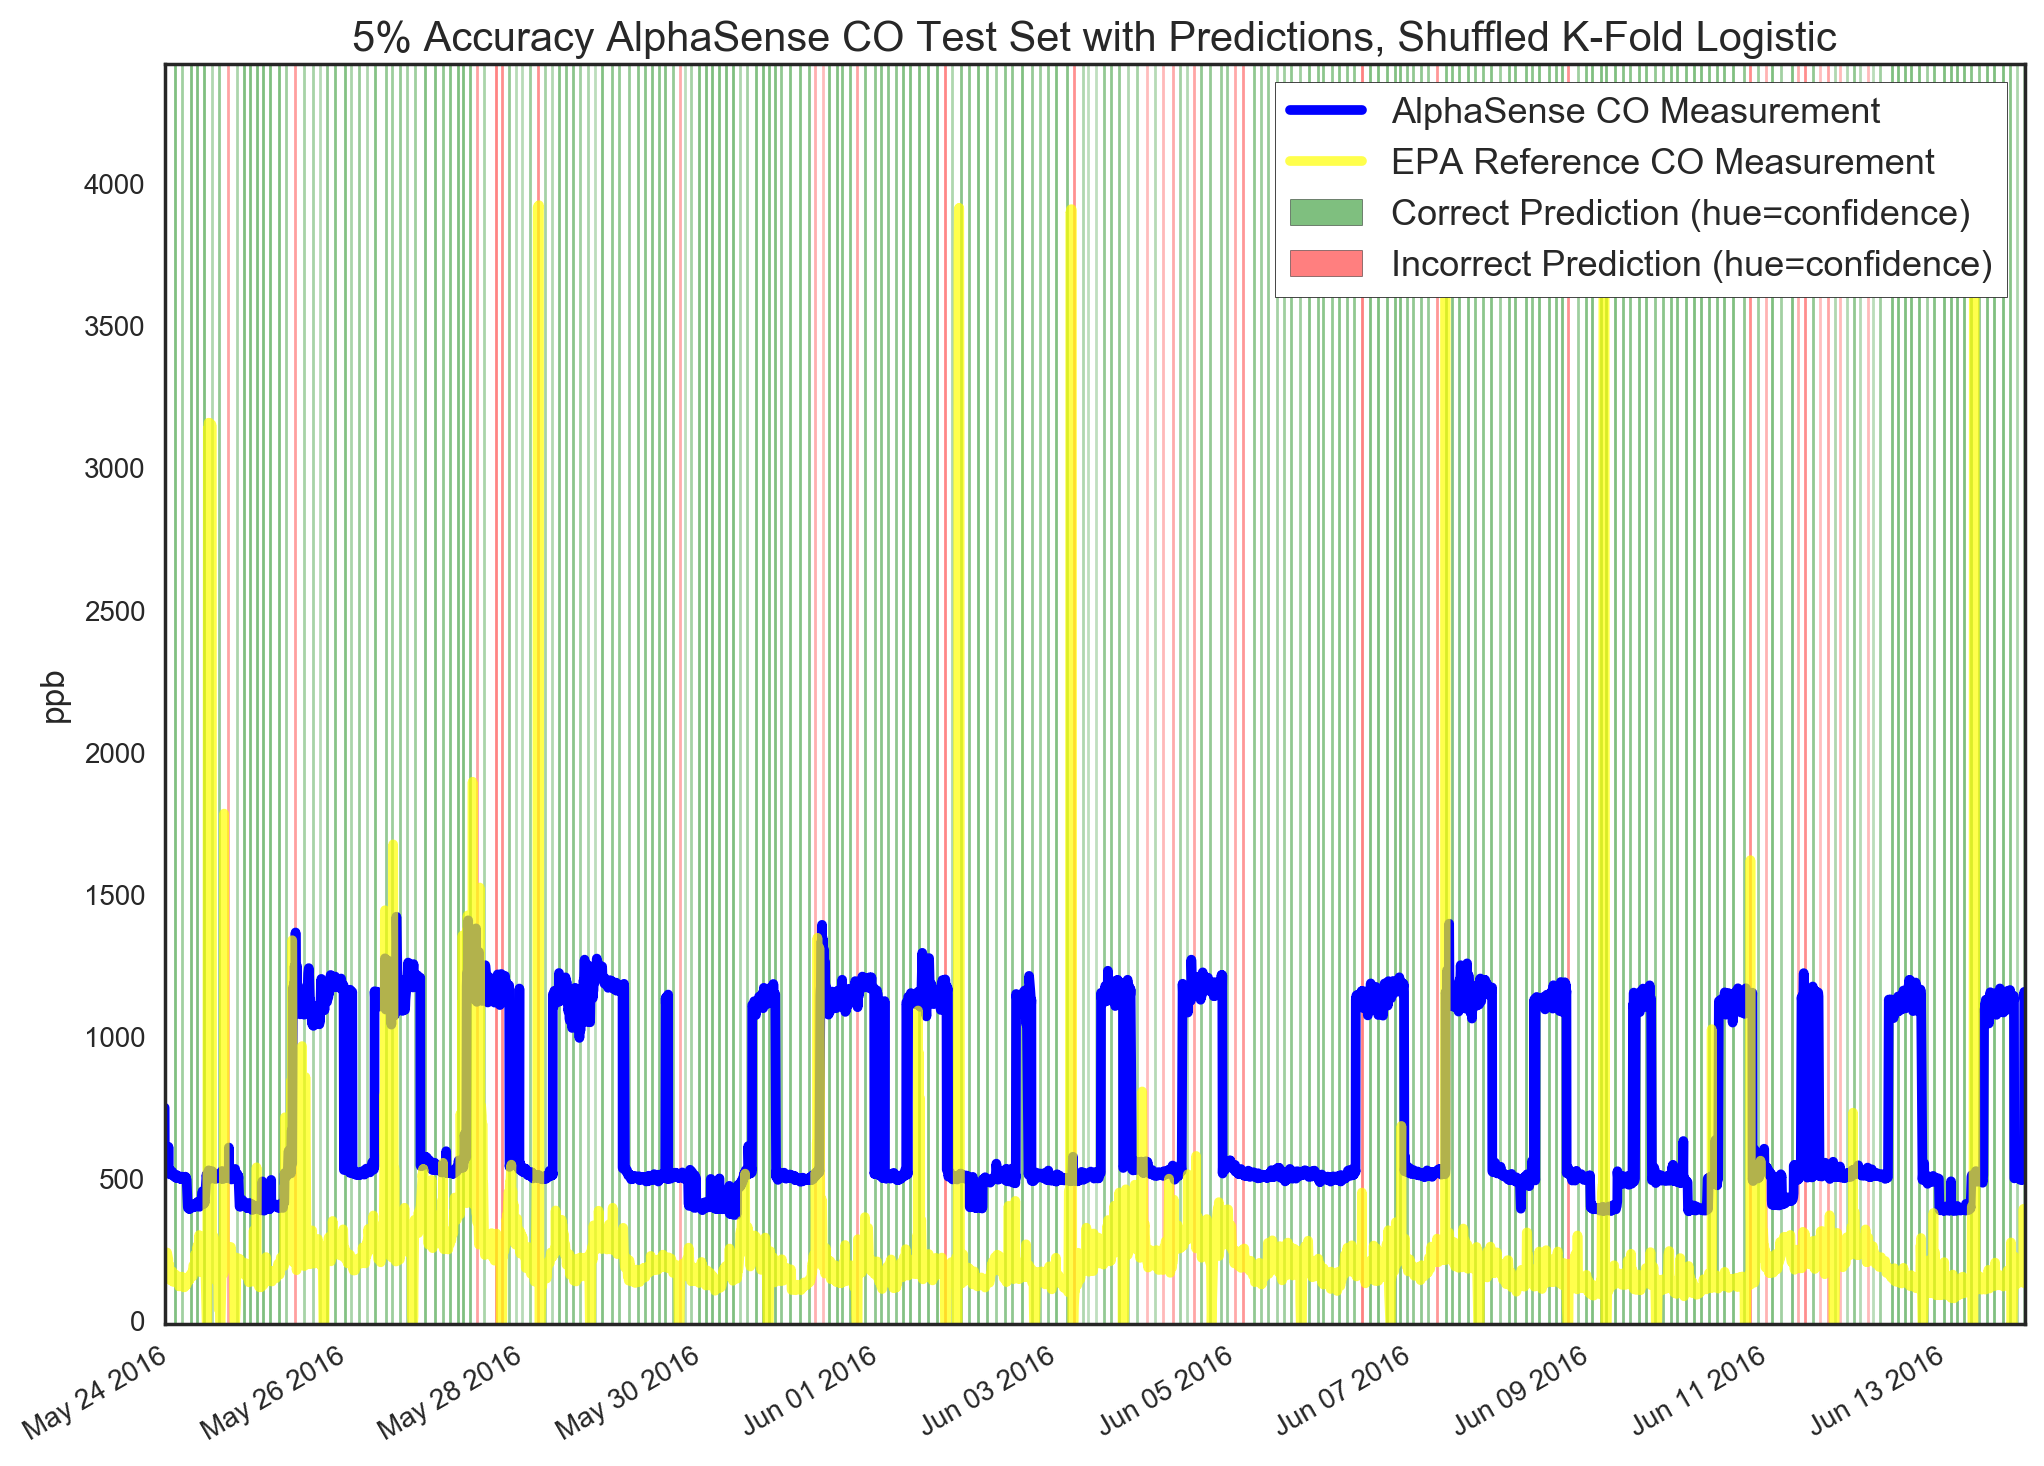
\includegraphics[width=\textwidth]{figs/as2_co_5_logistic_predictions}               
 	 \caption{AlphaSense CO Sensor #2 Prediction Accuracy}
  	\label{fig:as2_co_5_logistic_predictions}
\end{figure}



\FloatBarrier
\section{AlphaSense NO2}
\FloatBarrier

Following are additional plots from the AlphaSense NO2 test outlining the complete raw data and LMSE process, the accuracy with a tighter 4\% threshold, a visualization of the prediction accuracy and confidence, and the top 15 random forest selected features.

\begin{figure}[htb]
 	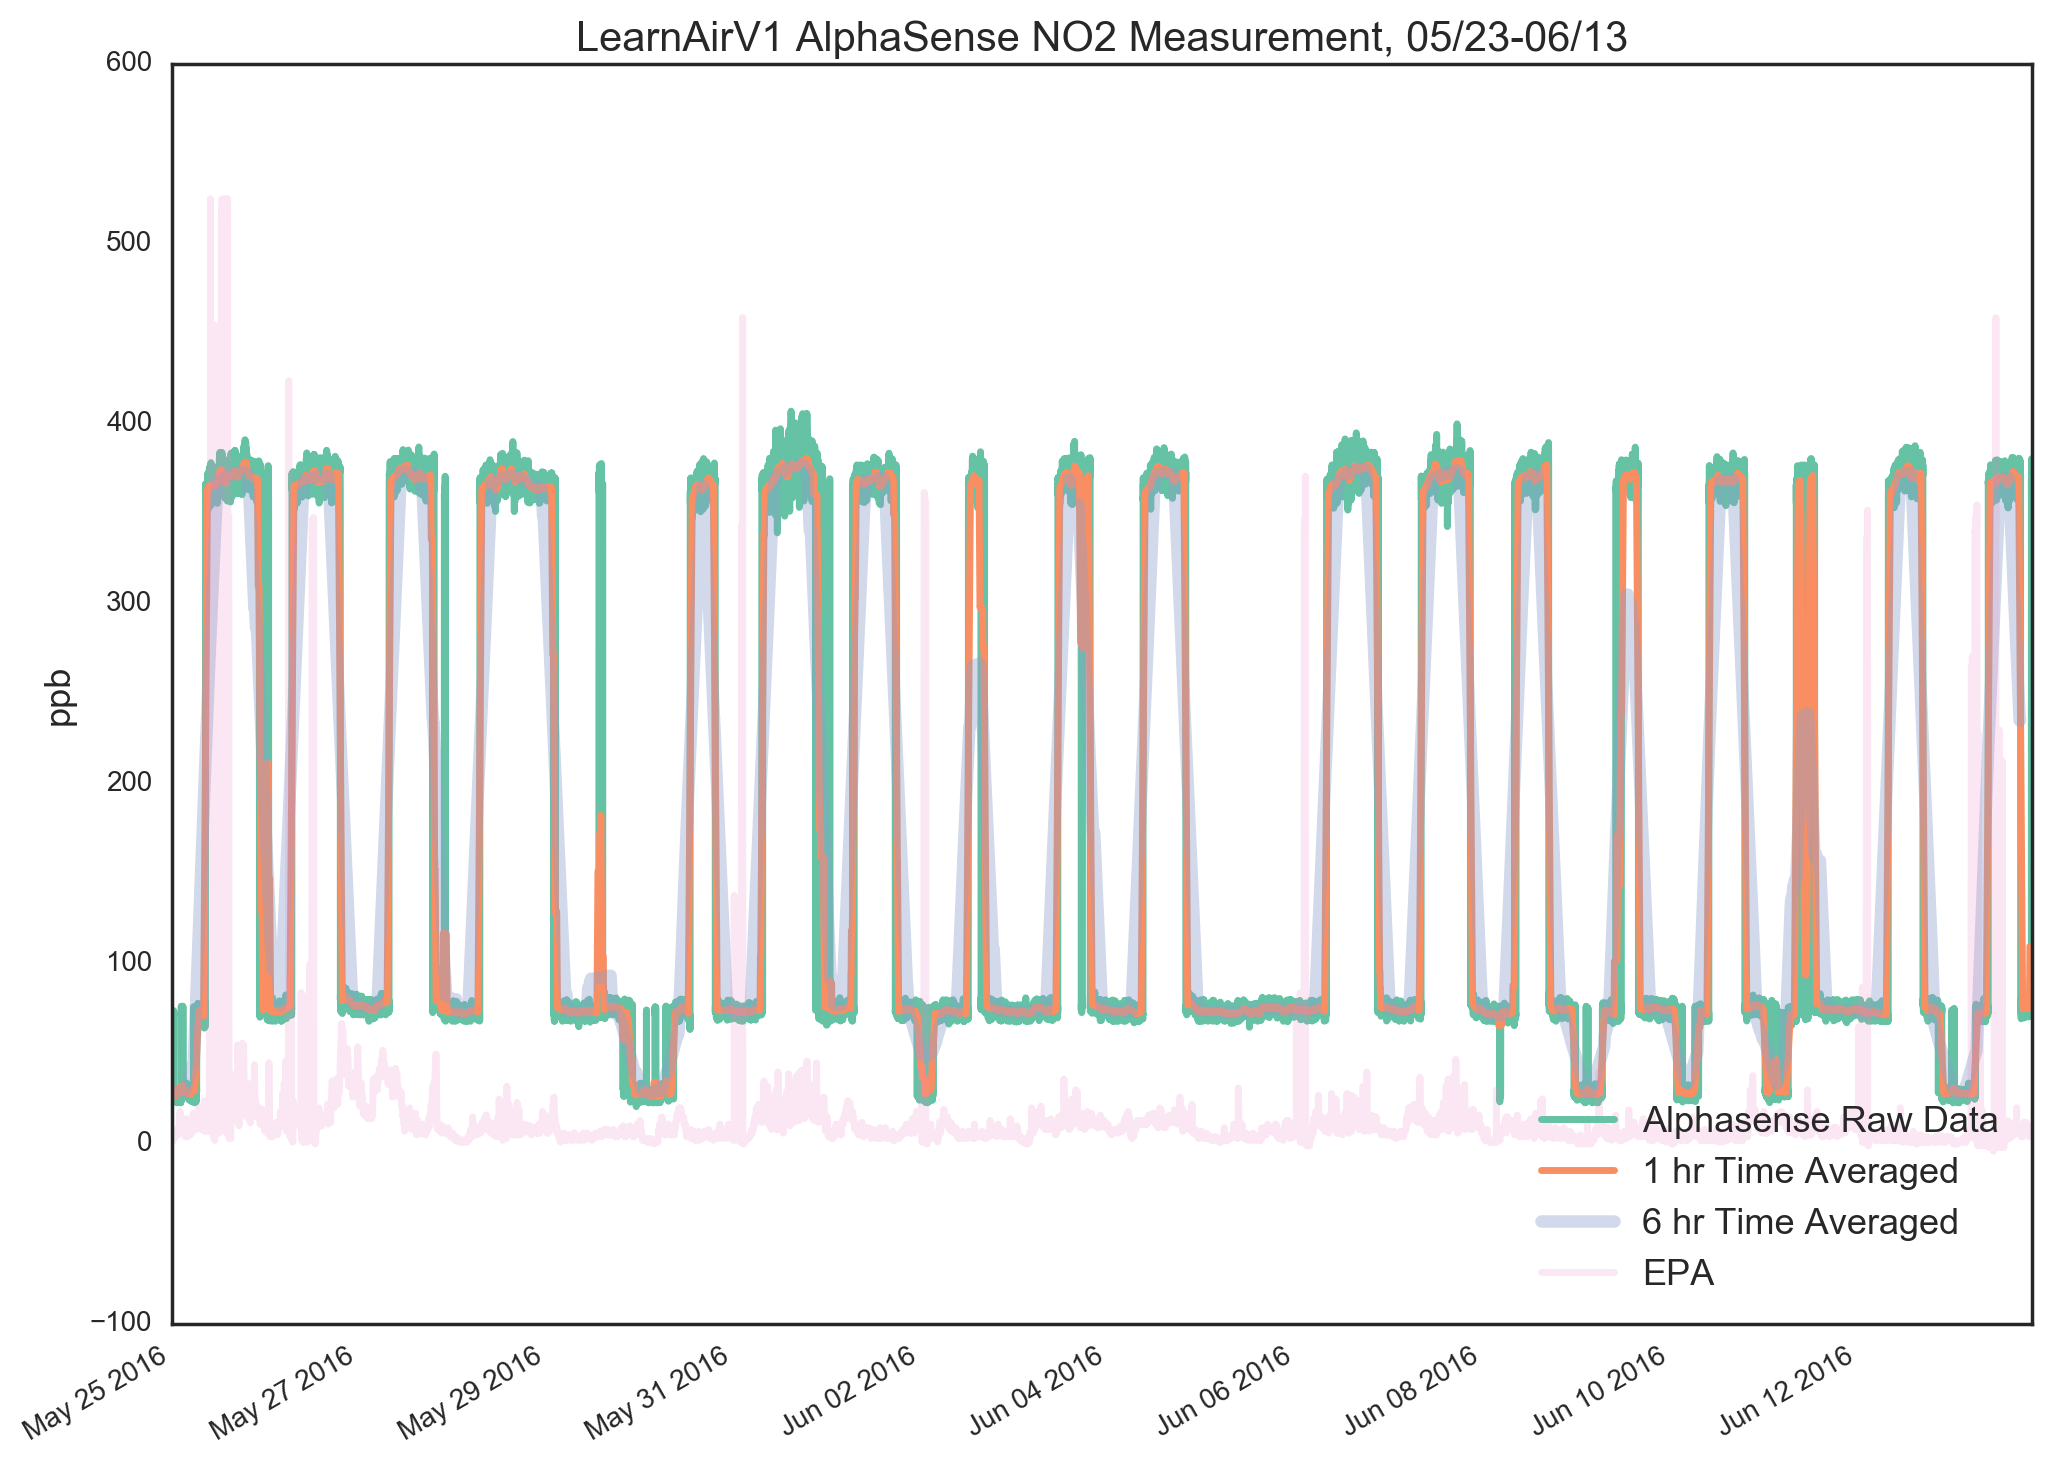
\includegraphics[width=\textwidth]{figs/as_no2_raw}               
 	 \caption{AlphaSense NO2 Raw Data}
  	\label{fig:as_no2_raw}
\end{figure}

\begin{figure}[htb]
 	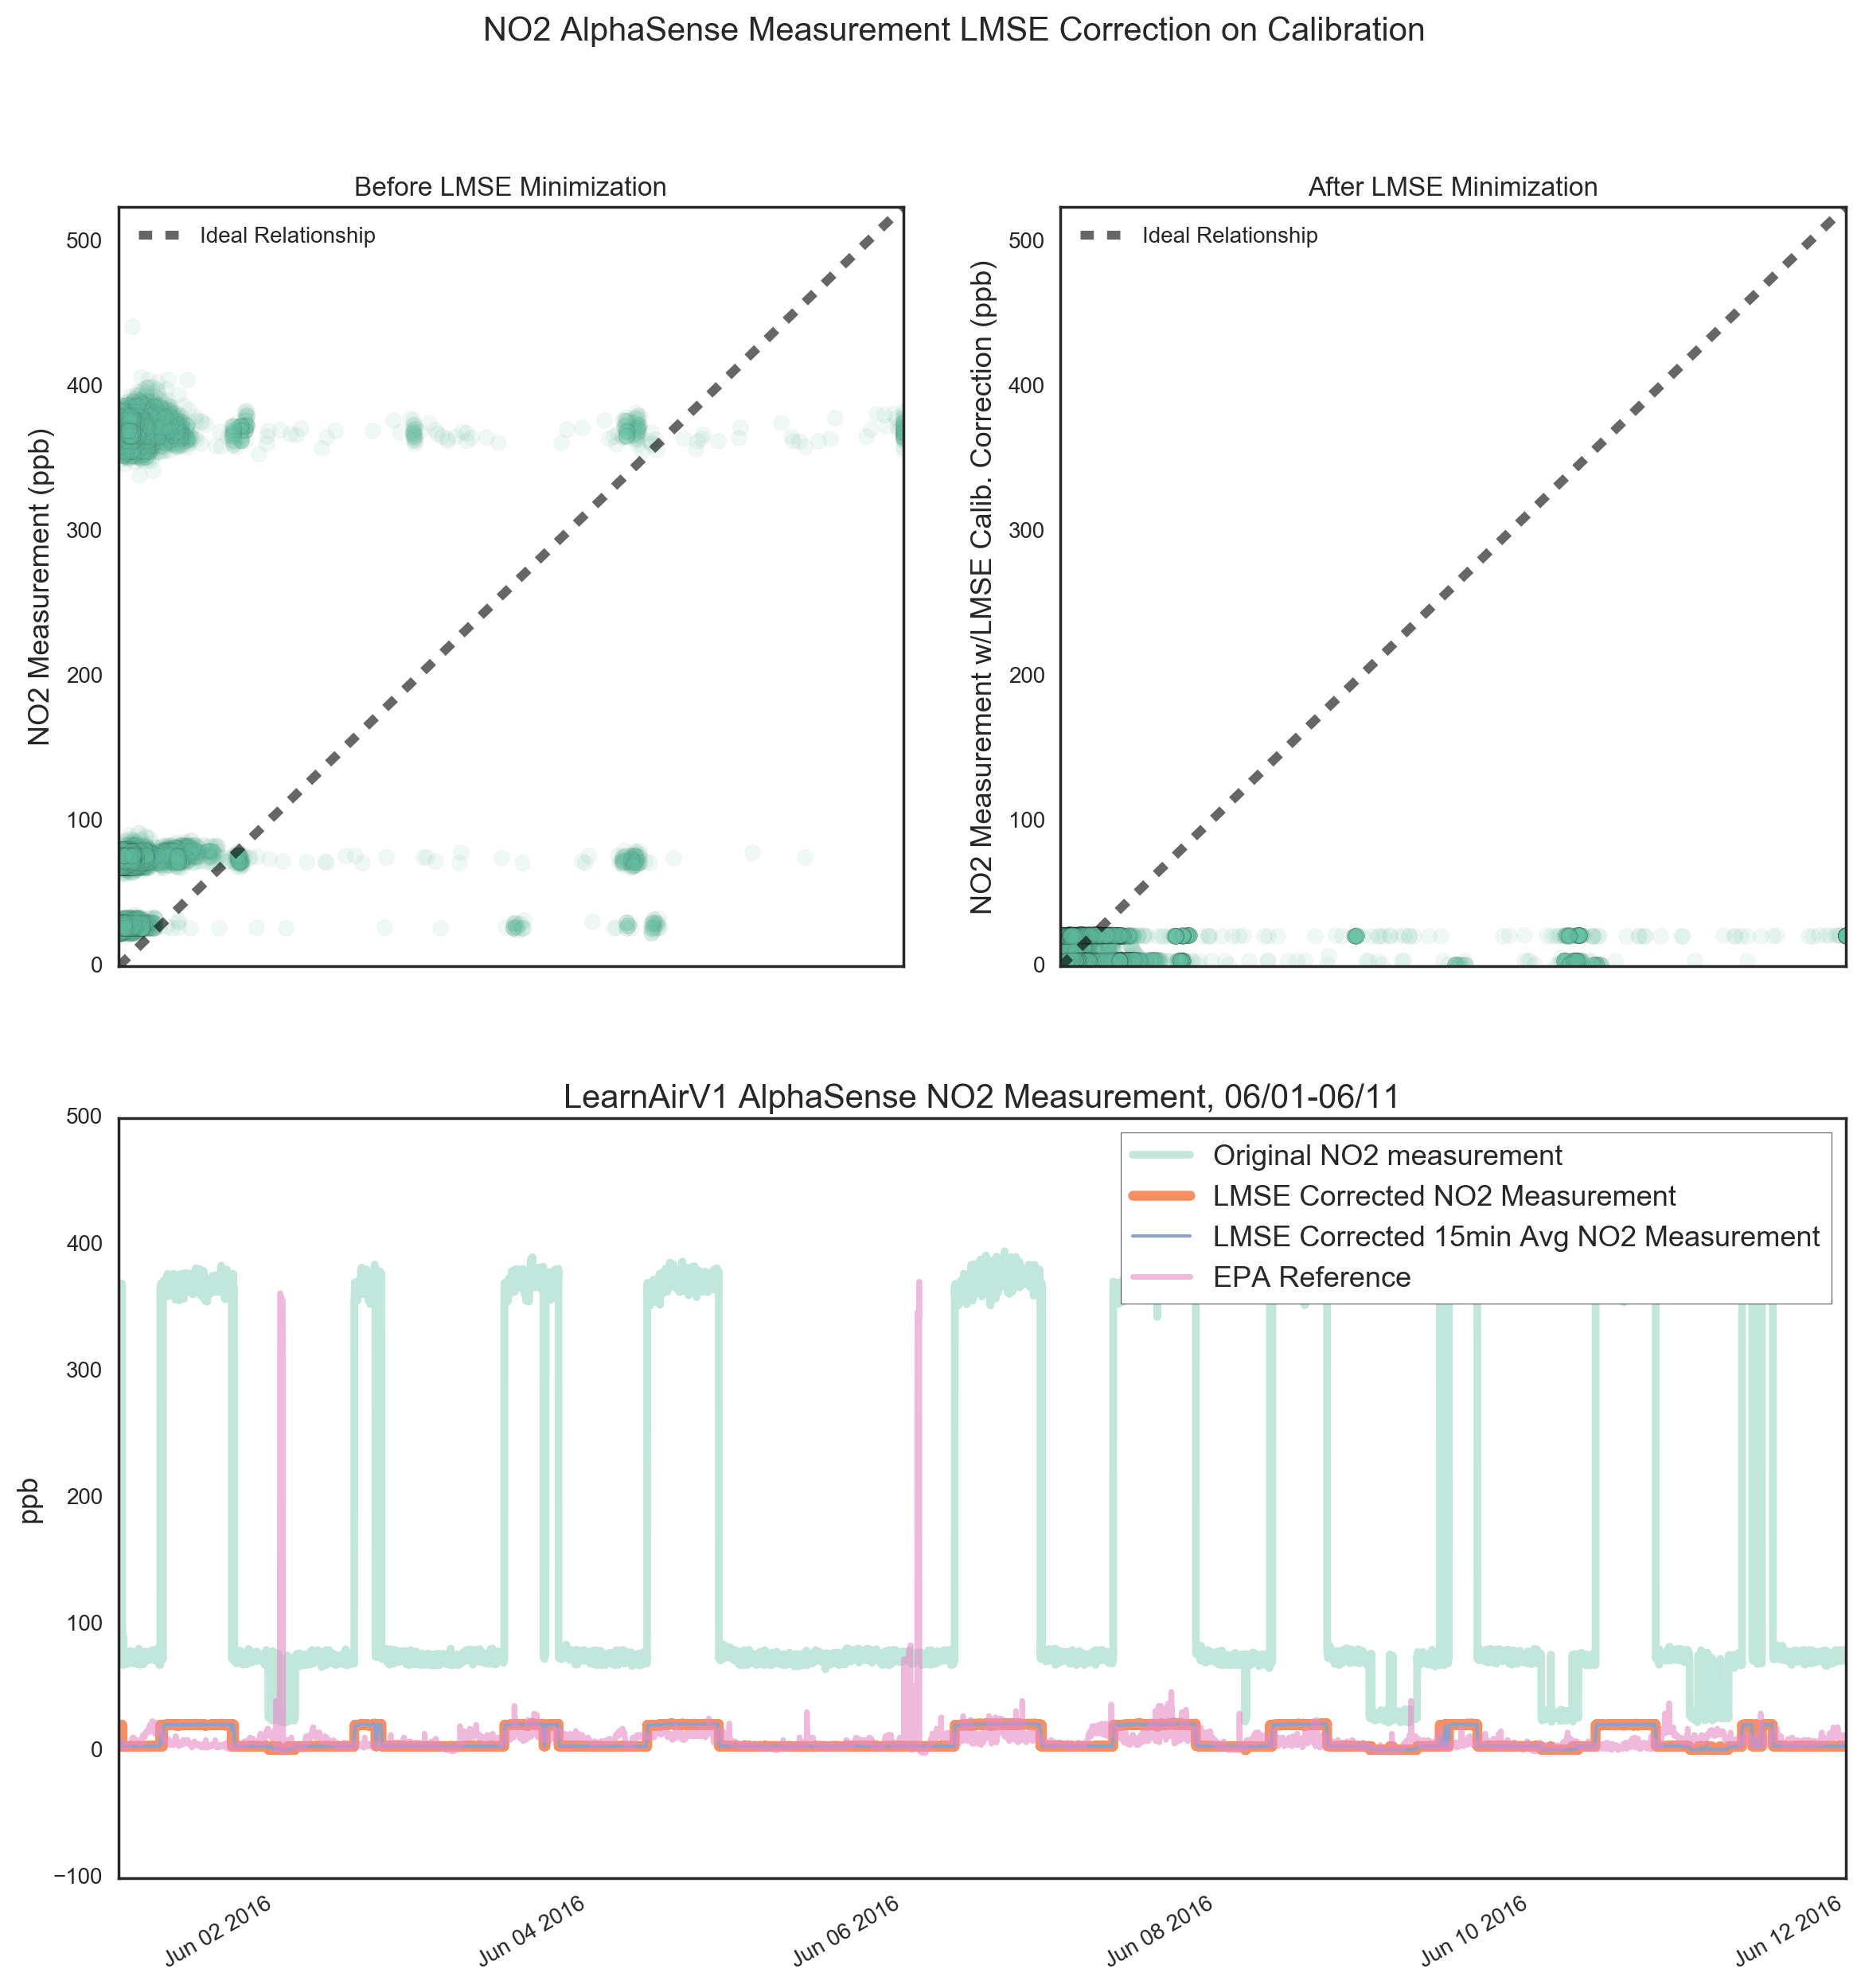
\includegraphics[width=\textwidth]{figs/as_no2_lmse}               
 	 \caption{AlphaSense NO2 after LMSE Calibration}
  	\label{fig:as_no2_lmse}
\end{figure}


\begin{figure}[htb]
 	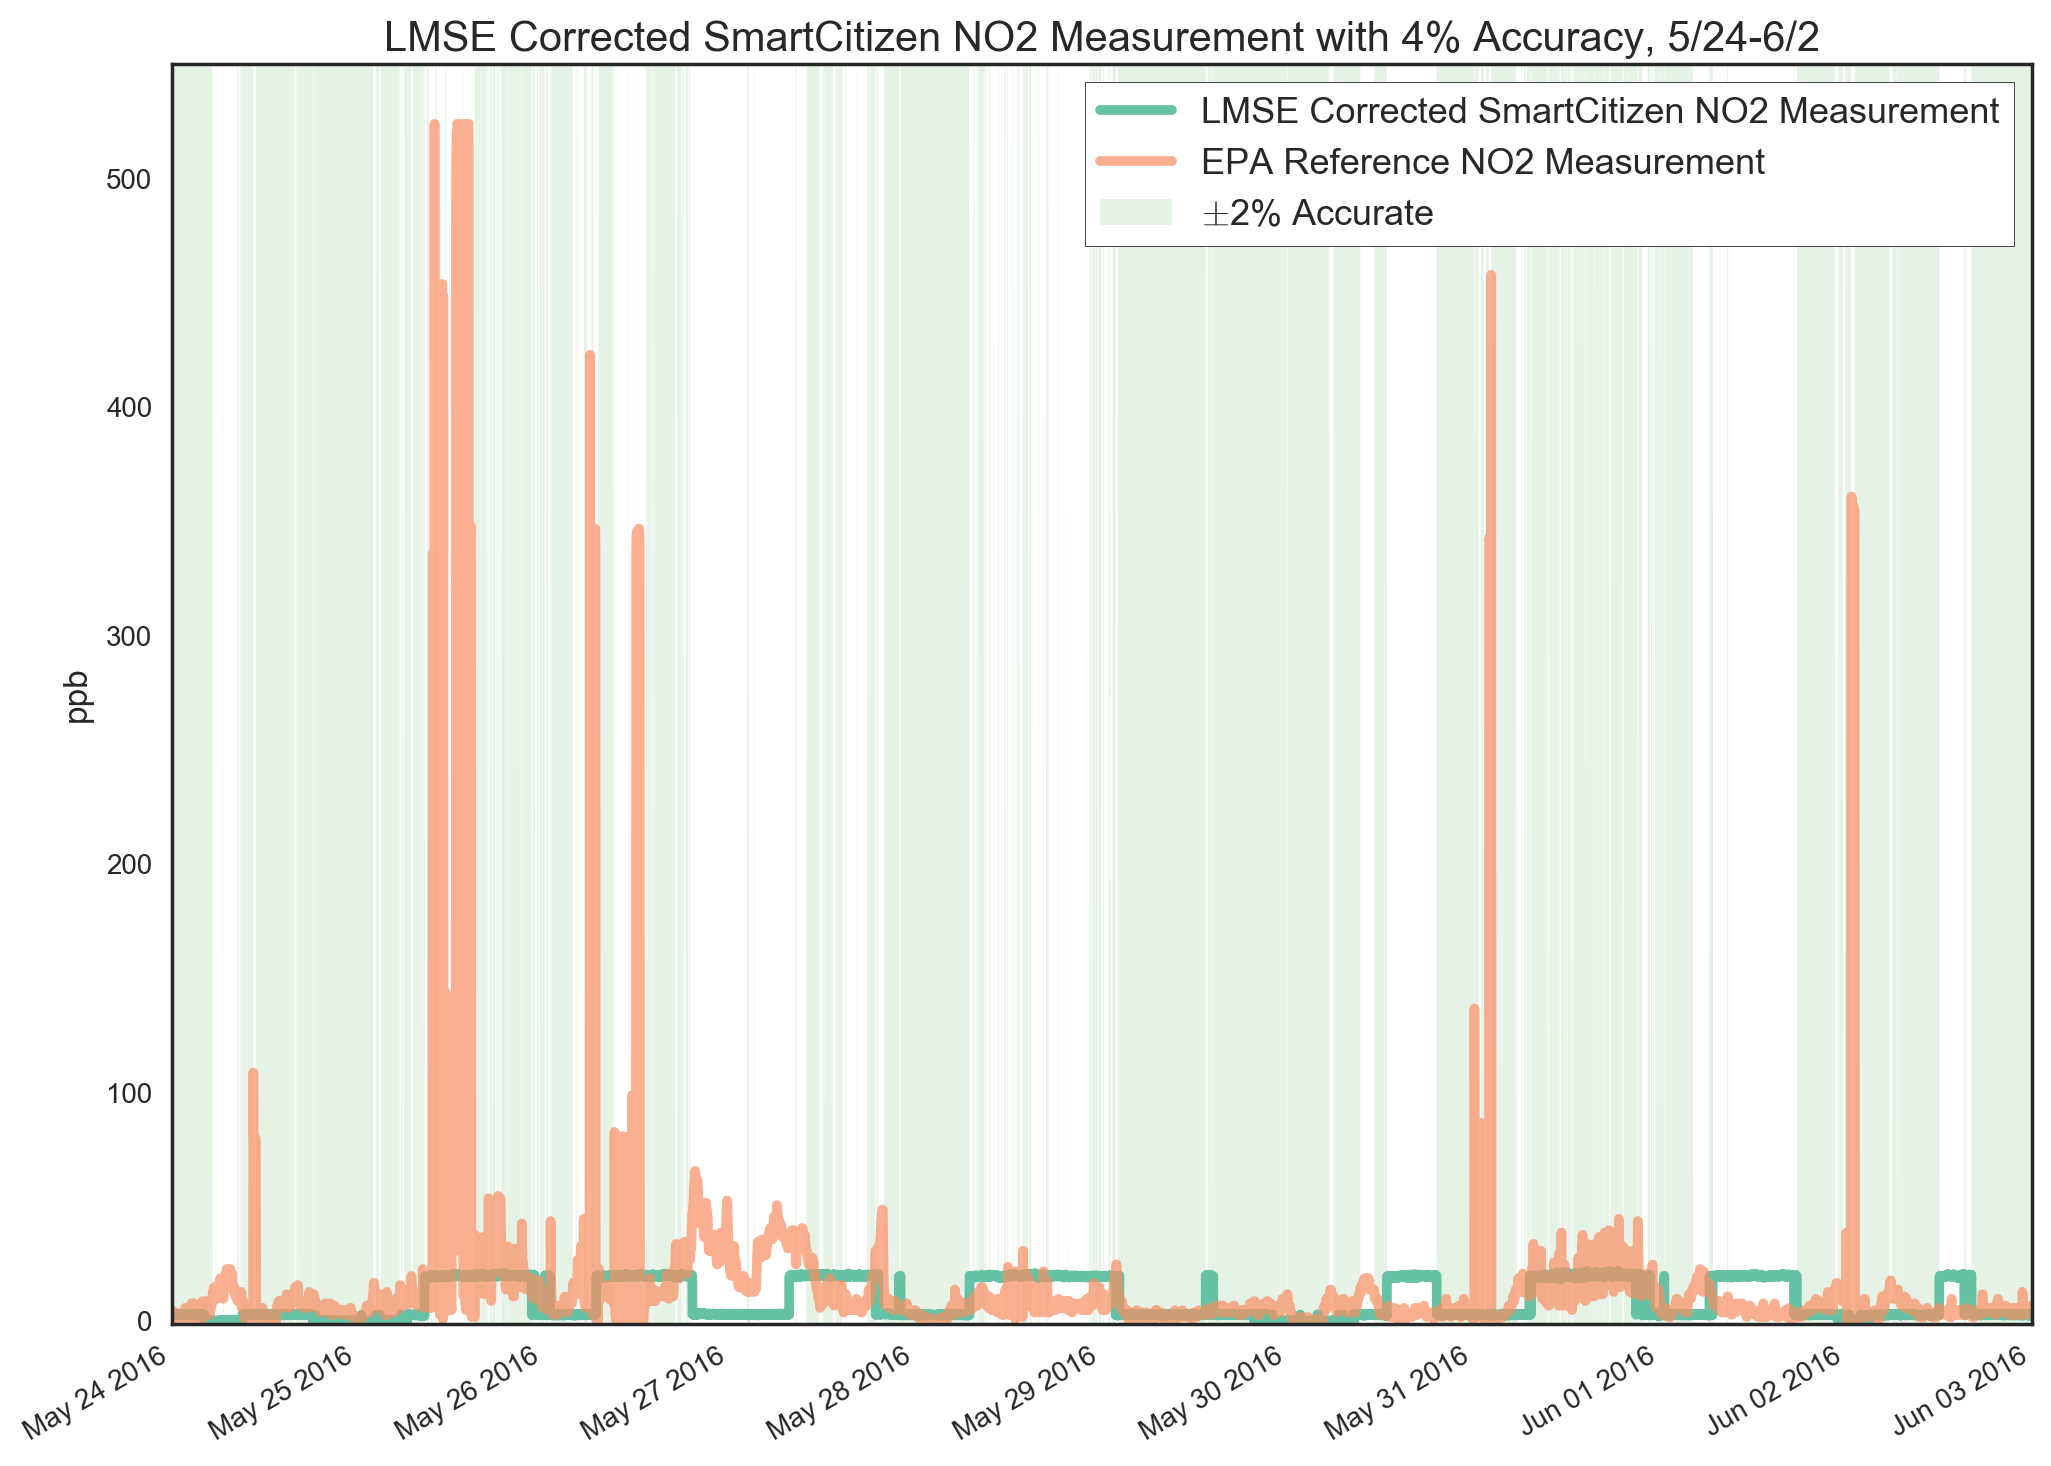
\includegraphics[width=\textwidth]{figs/as_no2_with_4_accuracy_zoomed}               
 	 \caption{AlphaSense NO2 with 4\% Accuracy Threshold}
  	\label{fig:as_no2_with_4_accuracy_zoomed}
\end{figure}


\begin{figure}[htb]
 	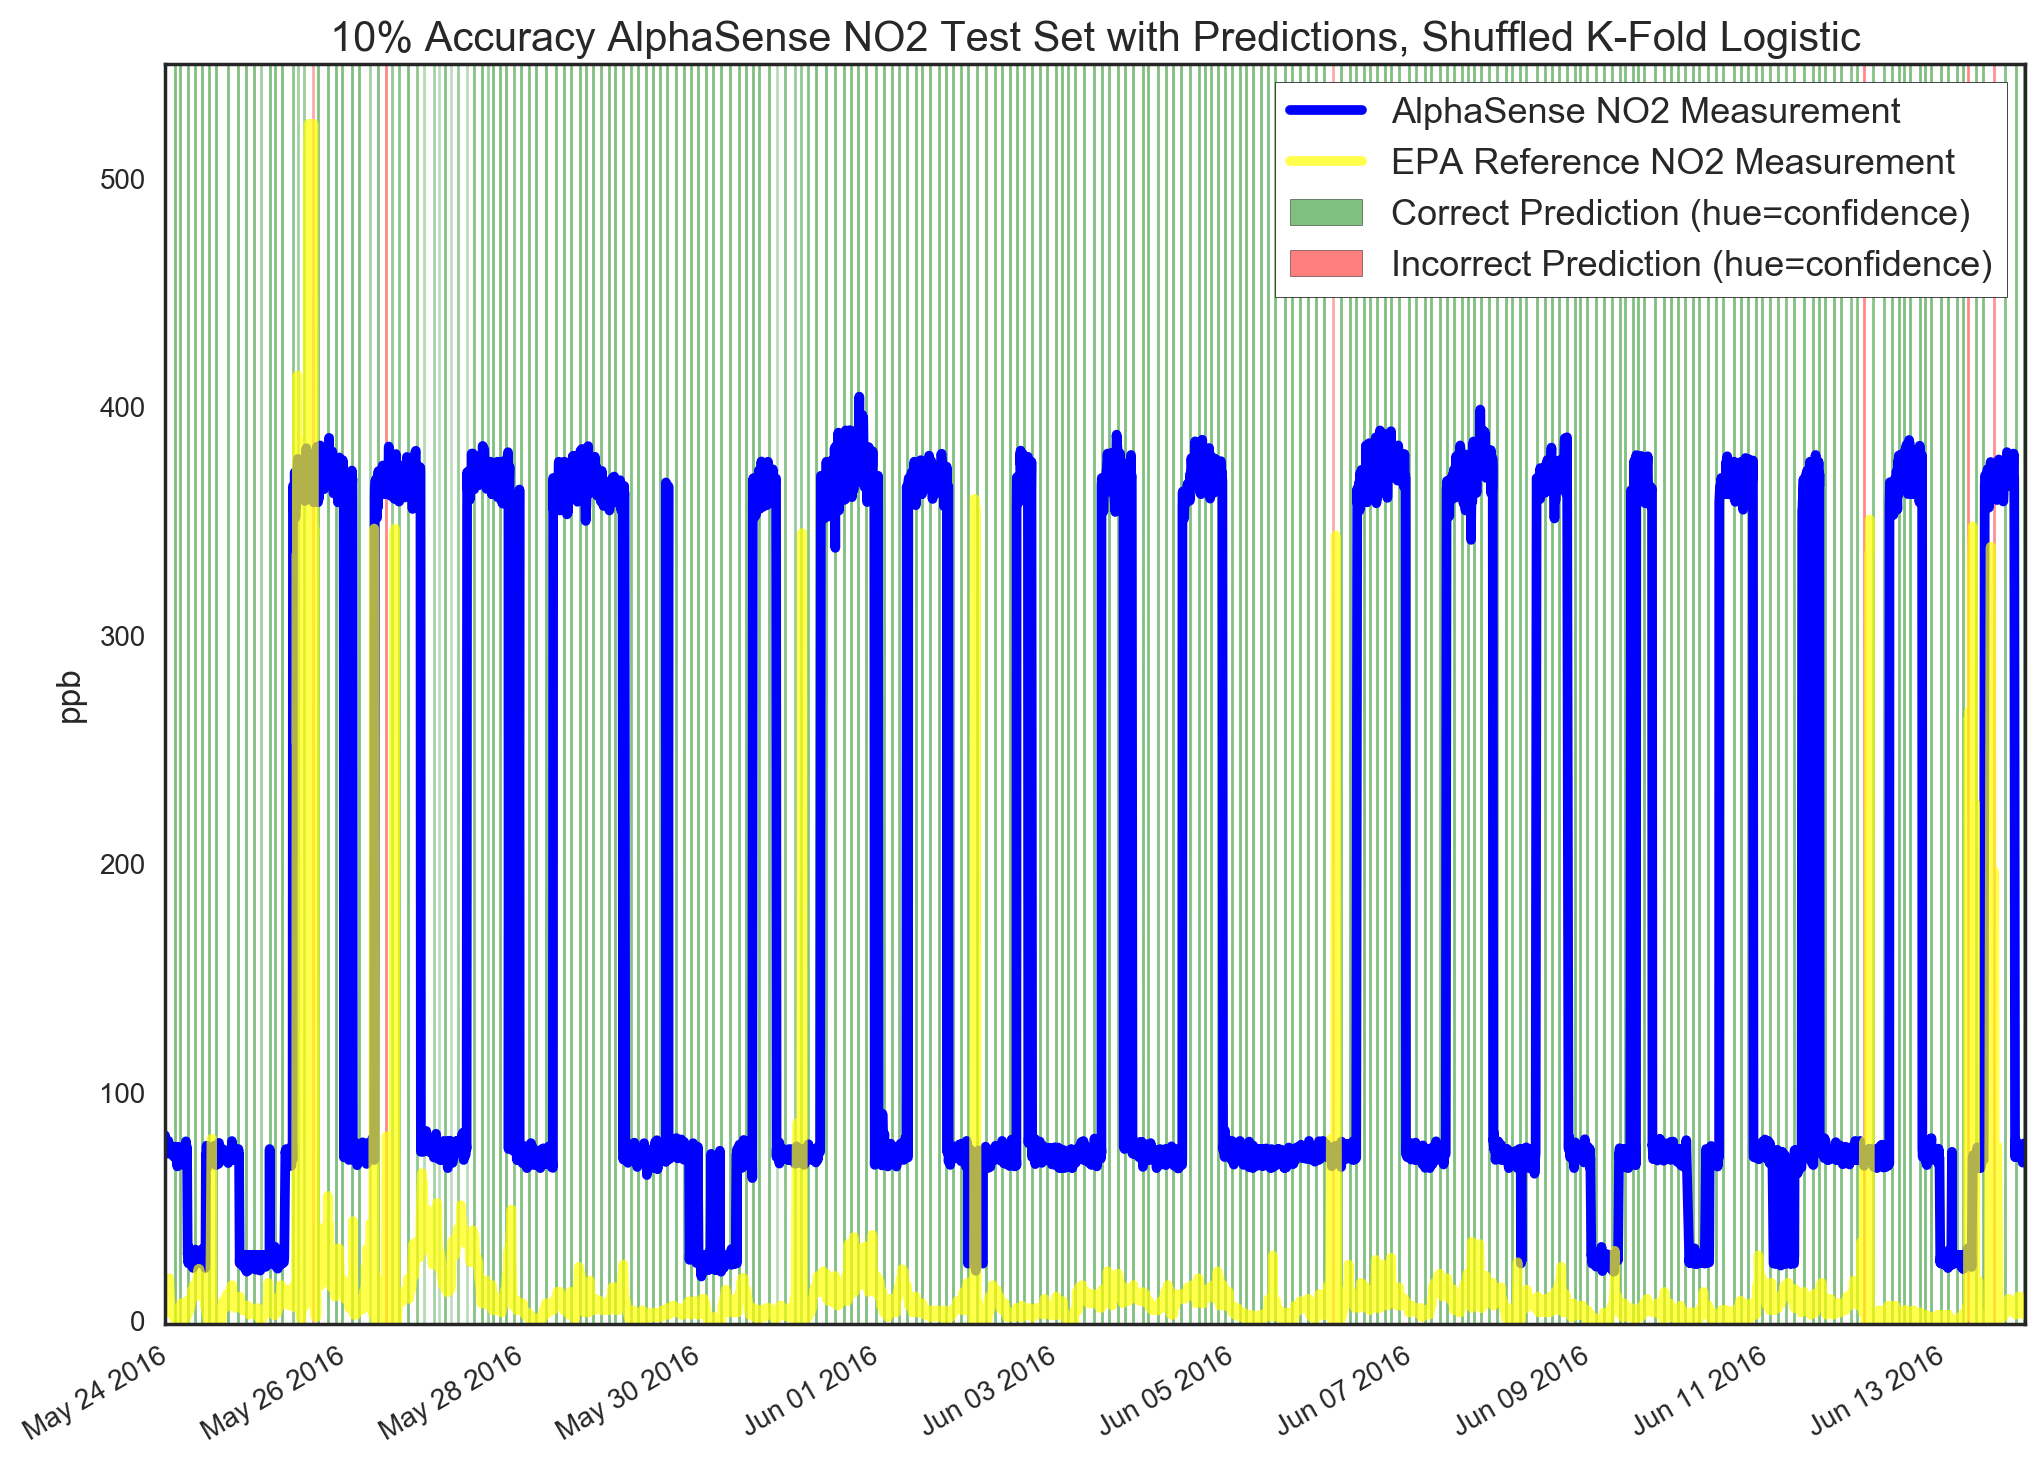
\includegraphics[width=\textwidth]{figs/as_no2_10_logistic_predictions}               
 	 \caption{AlphaSense NO2 Prediction Accuracy}
  	\label{fig:as_no2_10_logistic_predictions}
\end{figure}


\begin{table}[H]
\centering
\small
\begin{tabular}{lllllllll}
\\
\\
\toprule
Feature & Importance \\
\midrule
 avg\_60\_bkcarbon & 0.0422524706607 \\
 avg\_1440\_bkcarbon & 0.0417472204692 \\
 bkcarbon & 0.0385594210158 \\
 avg\_720\_bkcarbon & 0.0347584125412 \\
 min\_since\_plugged\_in & 0.0203302045169 \\
 avg\_60\_forecastio\_windSpeed & 0.0164269542704 \\
 derivative\_avg\_1440\_bkcarbon & 0.0162252088513 \\
 avg\_60\_forecastio\_windBearing & 0.0159723111776 \\
 avg\_1440\_lmse\_calib\_as\_co & 0.0149001557286 \\
 avg\_720\_lmse\_scaled\_sharpDust & 0.0148211173957 \\
 day\_of\_year & 0.0145567862081 \\
 avg\_60\_forecastio\_pressure & 0.0142569975814 \\
 daily\_avg\_sck\_humidity & 0.013849933762 \\
 avg\_30\_ws & 0.0137791673751 \\
 daily\_avg\_forecastio\_temperature & 0.0136871069105 \\
\bottomrule
\end{tabular}
\label{tab:as_no2_randomforest_features}
\caption{Top 15 Features from Random Forest for AlphaSense NO2, used in Pruned Logistic Regression}
\end{table}

Figure \ref{fig:as_no2_10_roc_pruned_features} is the ROC using just the top 15 features to predict NO2.

\begin{figure}[htb]
 	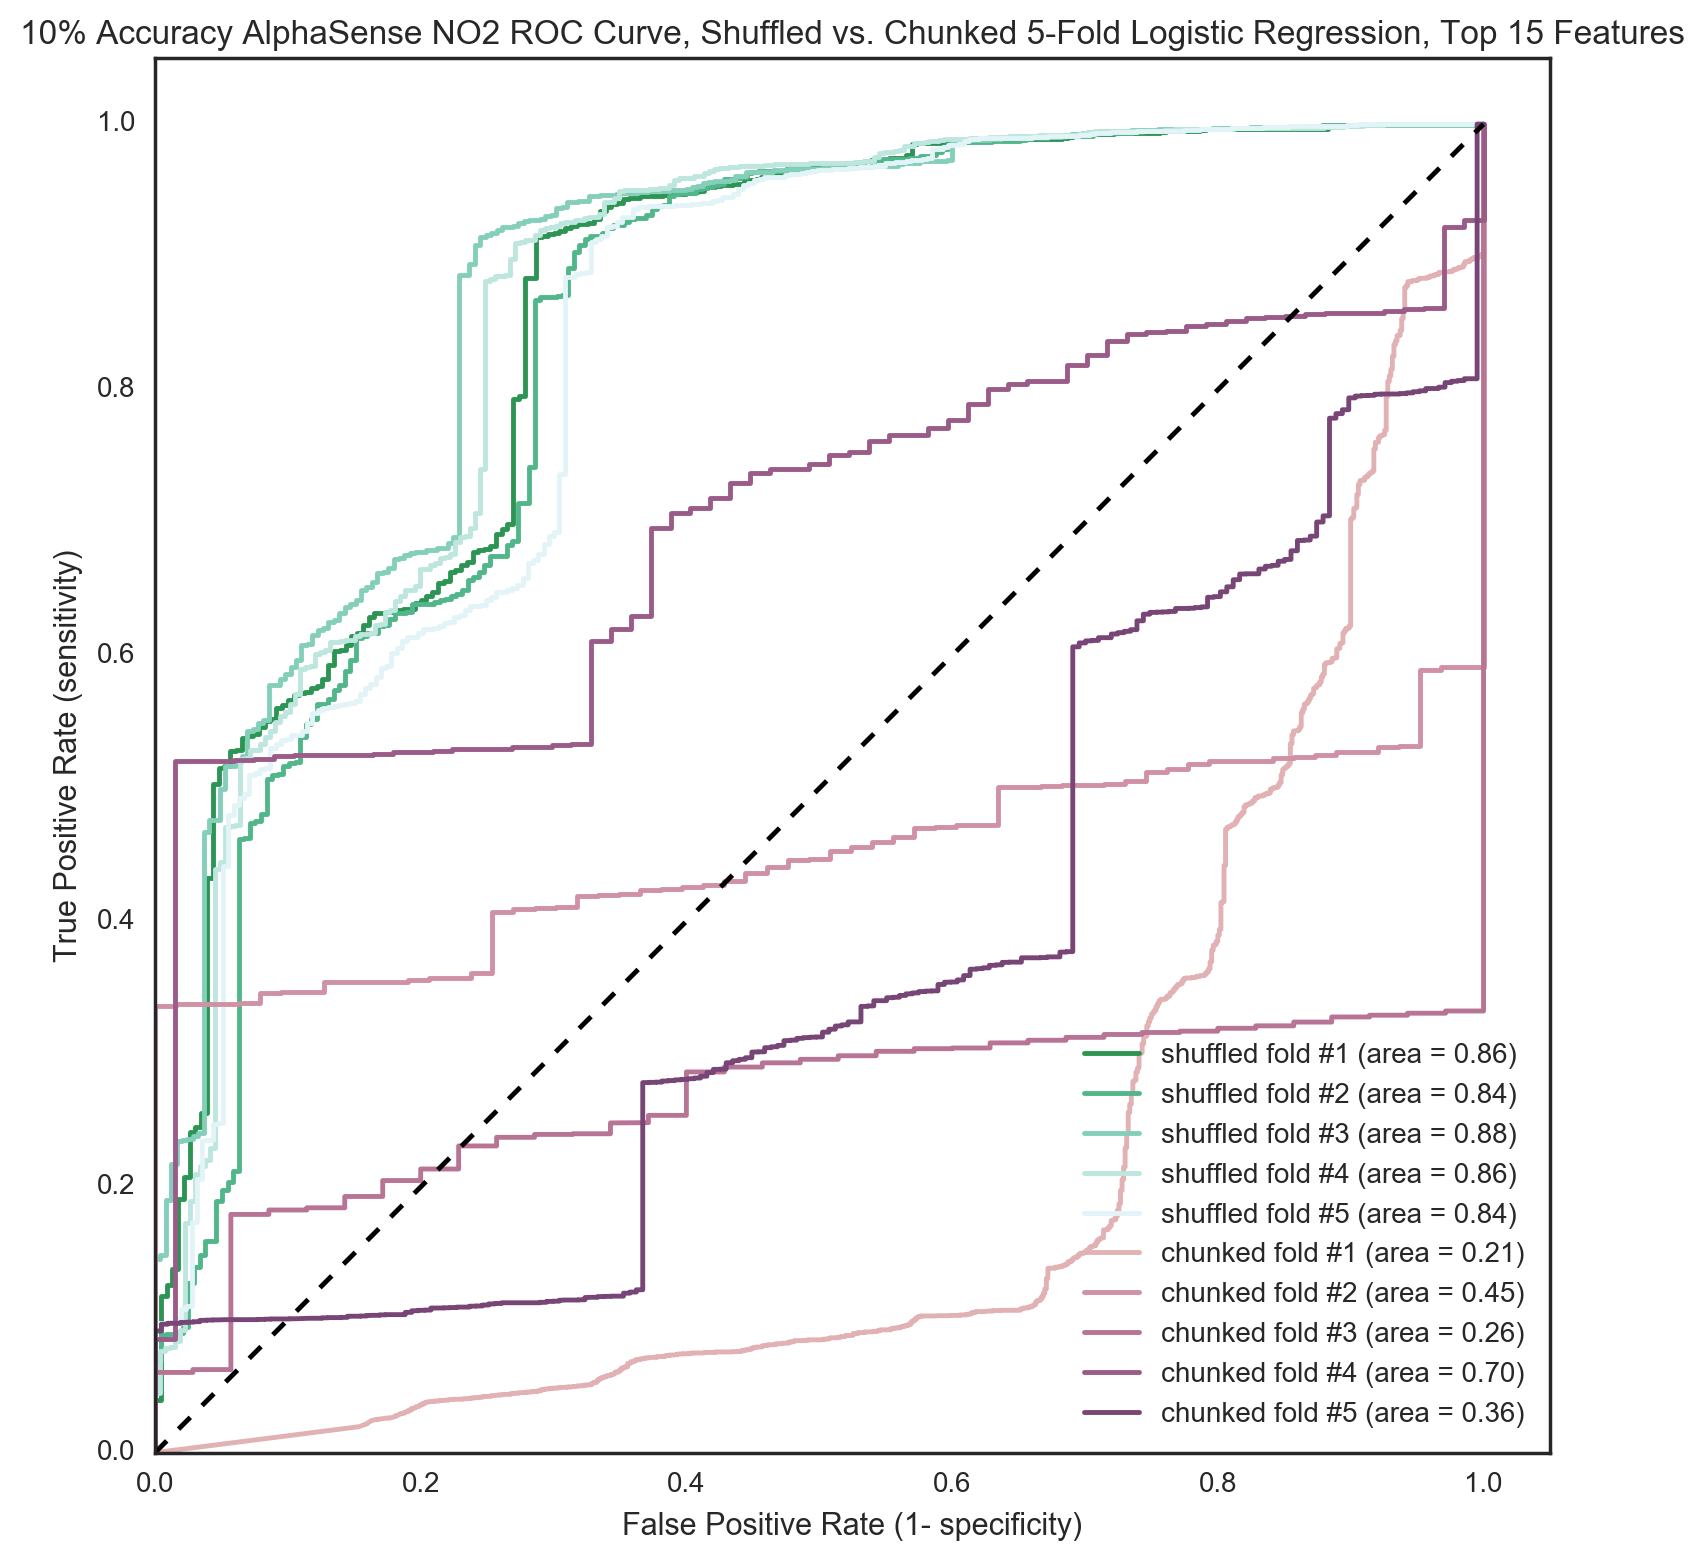
\includegraphics[width=\textwidth]{figs/as_no2_10_roc_pruned_features}               
 	 \caption{AlphaSense NO2 ROC Using Top 15 Features}
  	\label{fig:as_no2_10_roc_pruned_features}
\end{figure}


\FloatBarrier
\section{AlphaSense O3}
\FloatBarrier

Following are additional plots from the AlphaSense O3 test outlining the complete raw data and LMSE process, the accuracy with a tighter 7.5\% threshold, a visualization of the prediction accuracy and confidence, and the top 15 random forest selected features for both sensors tested.  Additionally, the ROC plots using just the top 15 features is included for both sensors.

\begin{figure}[htb]
 	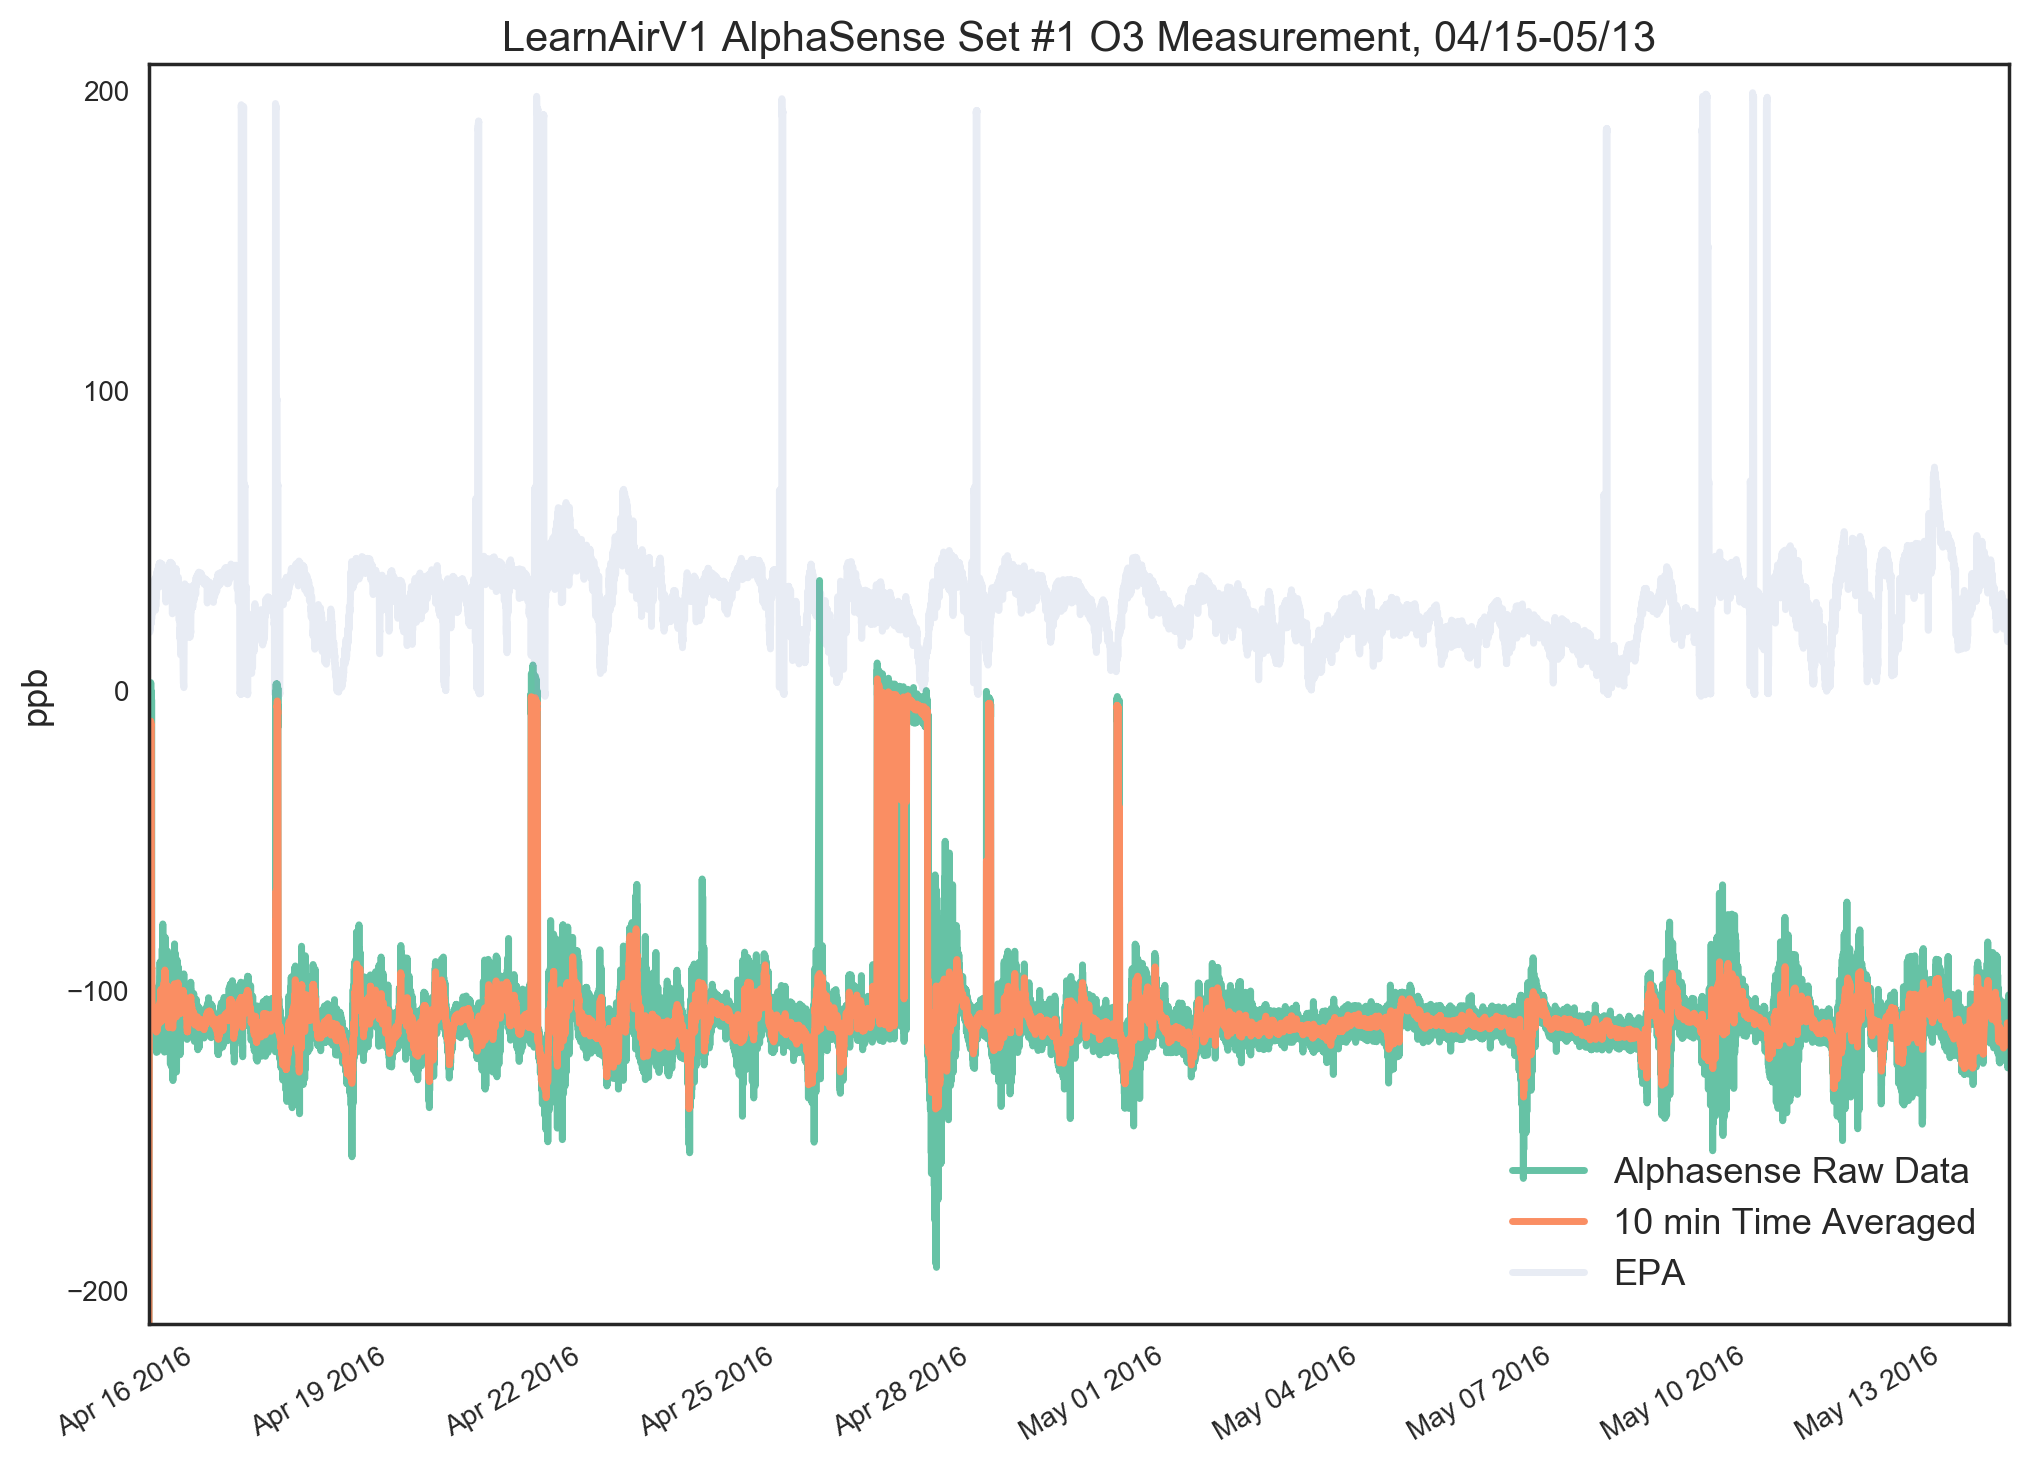
\includegraphics[width=\textwidth]{figs/as1_o3_raw}               
 	 \caption{AlphaSense O3 Sensor #1 Raw Data}
  	\label{fig:as1_o3_raw}
\end{figure}

\begin{figure}[htb]
 	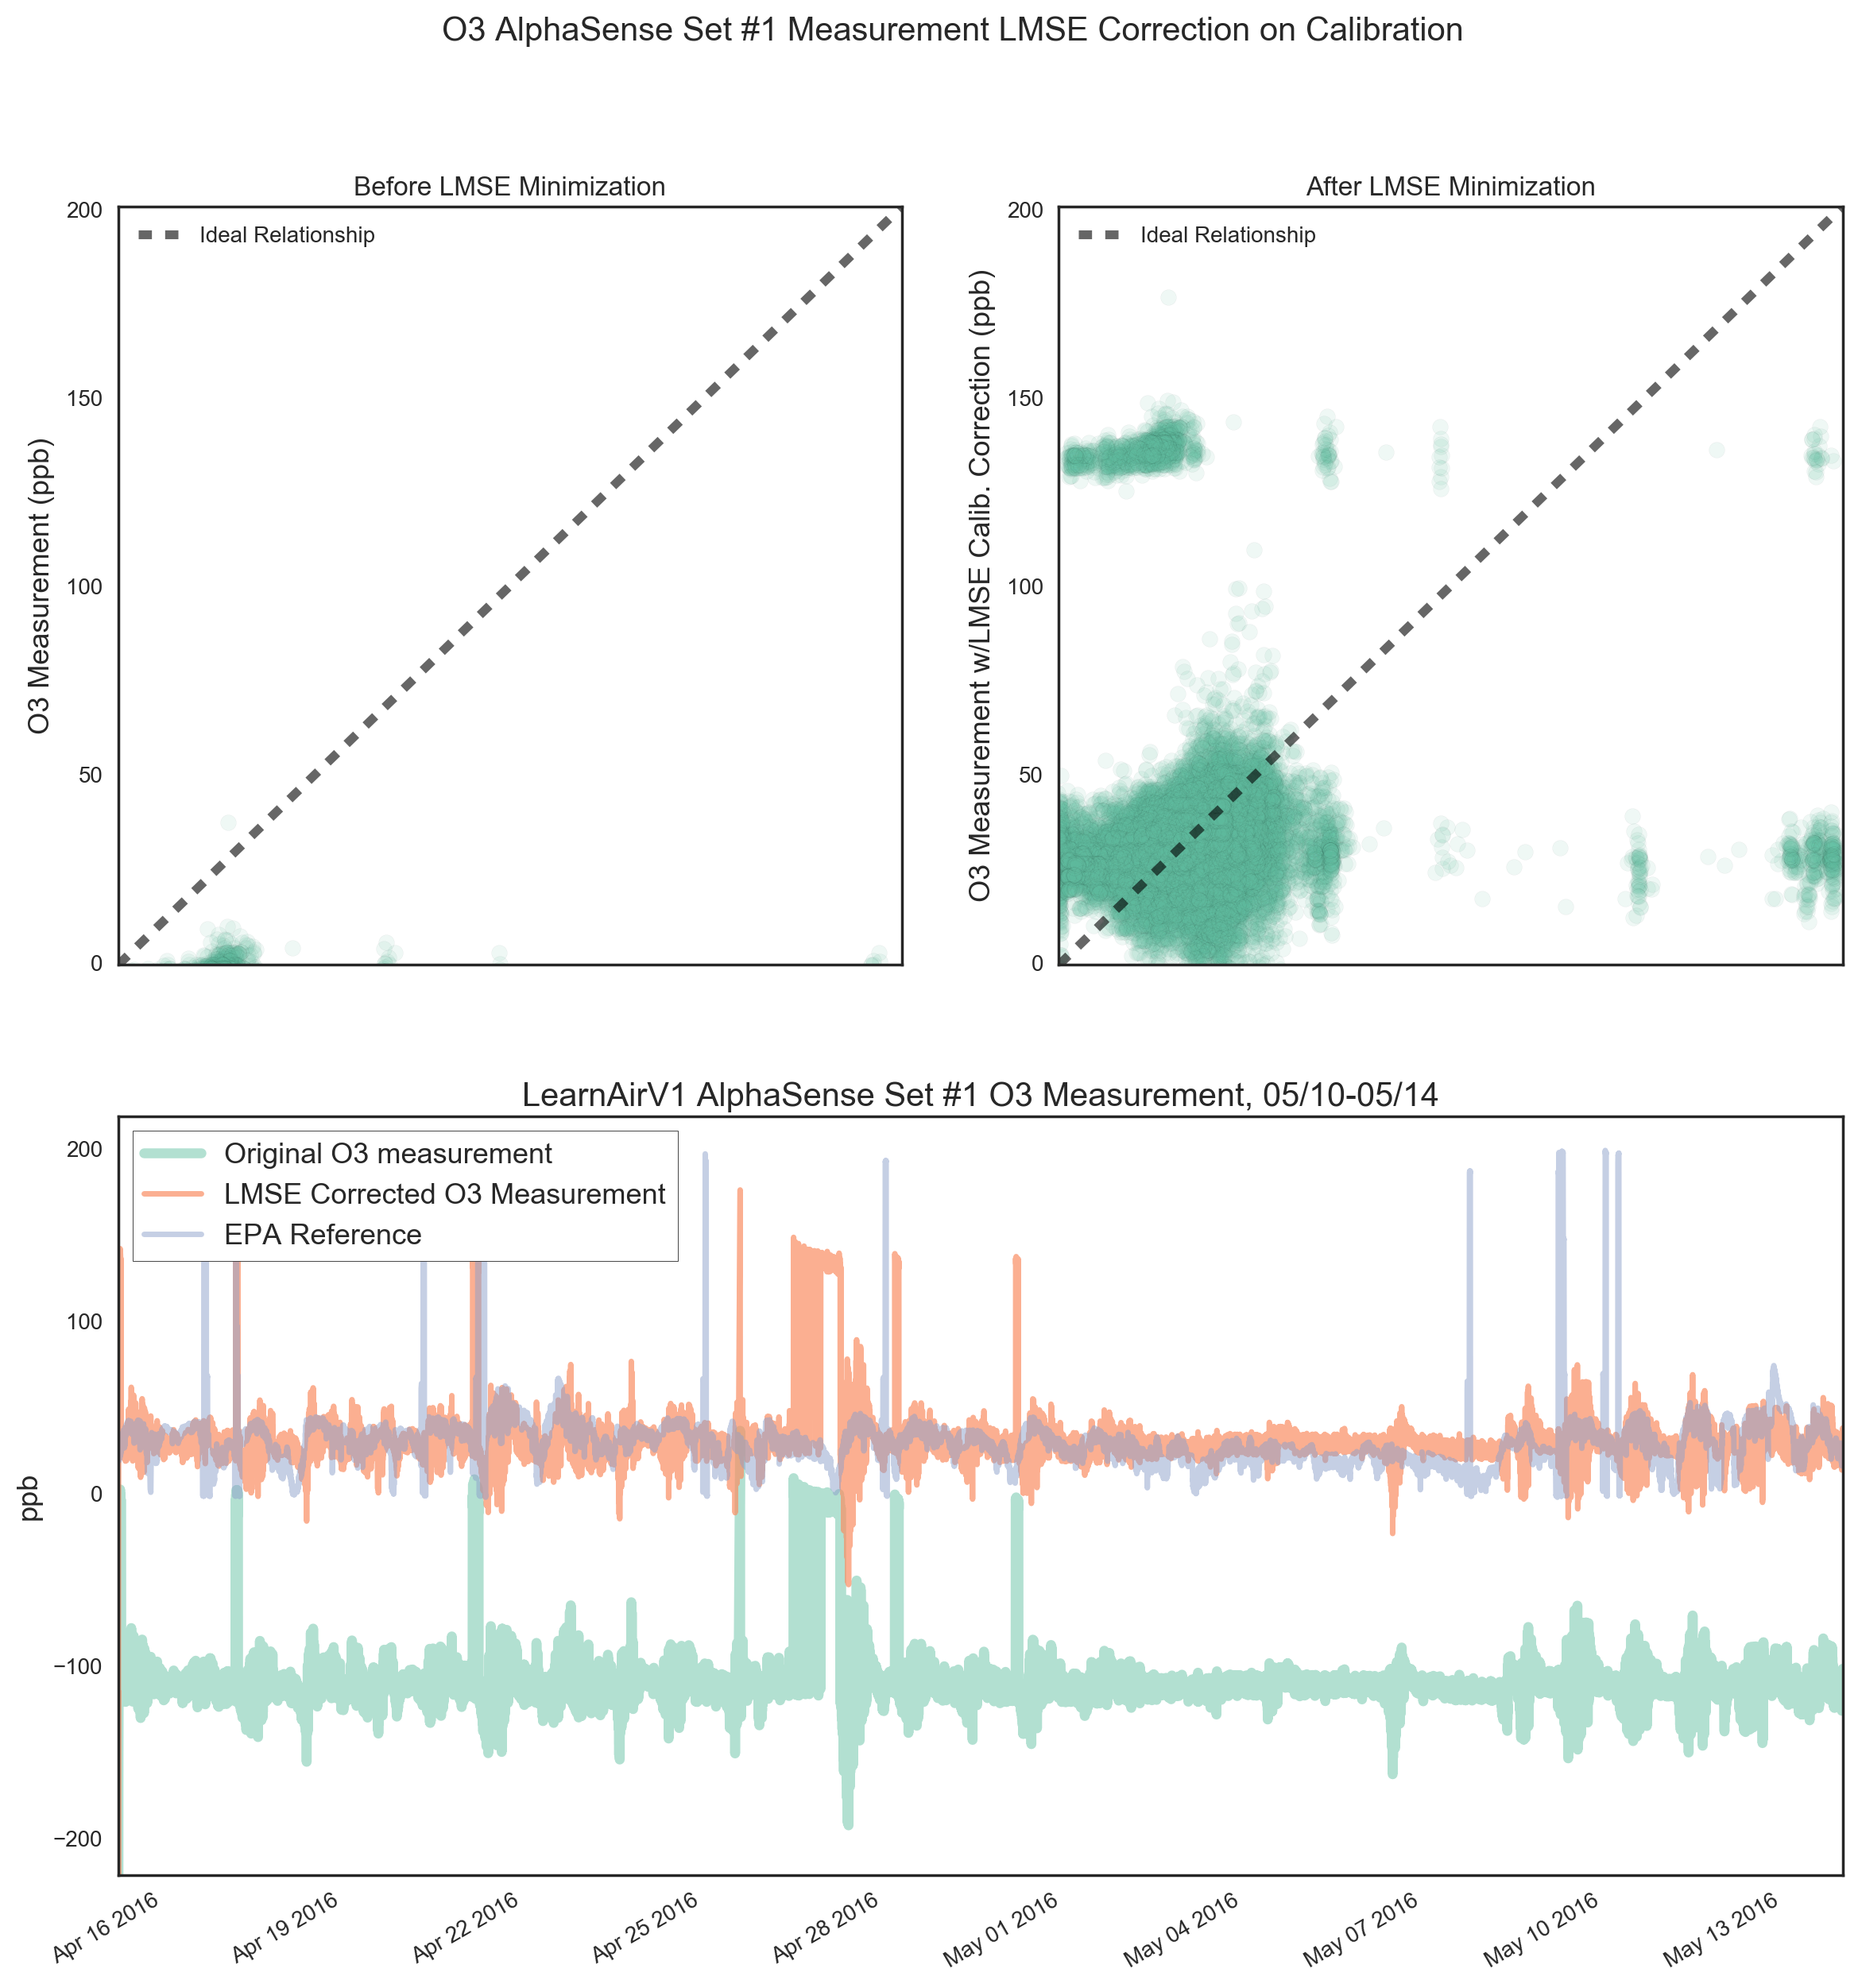
\includegraphics[width=\textwidth]{figs/as1_o3_lmse}               
 	 \caption{AlphaSense O3 Sensor #1 after LMSE Calibration}
  	\label{fig:as1_o3_lmse}
\end{figure}

\begin{figure}[htb]
 	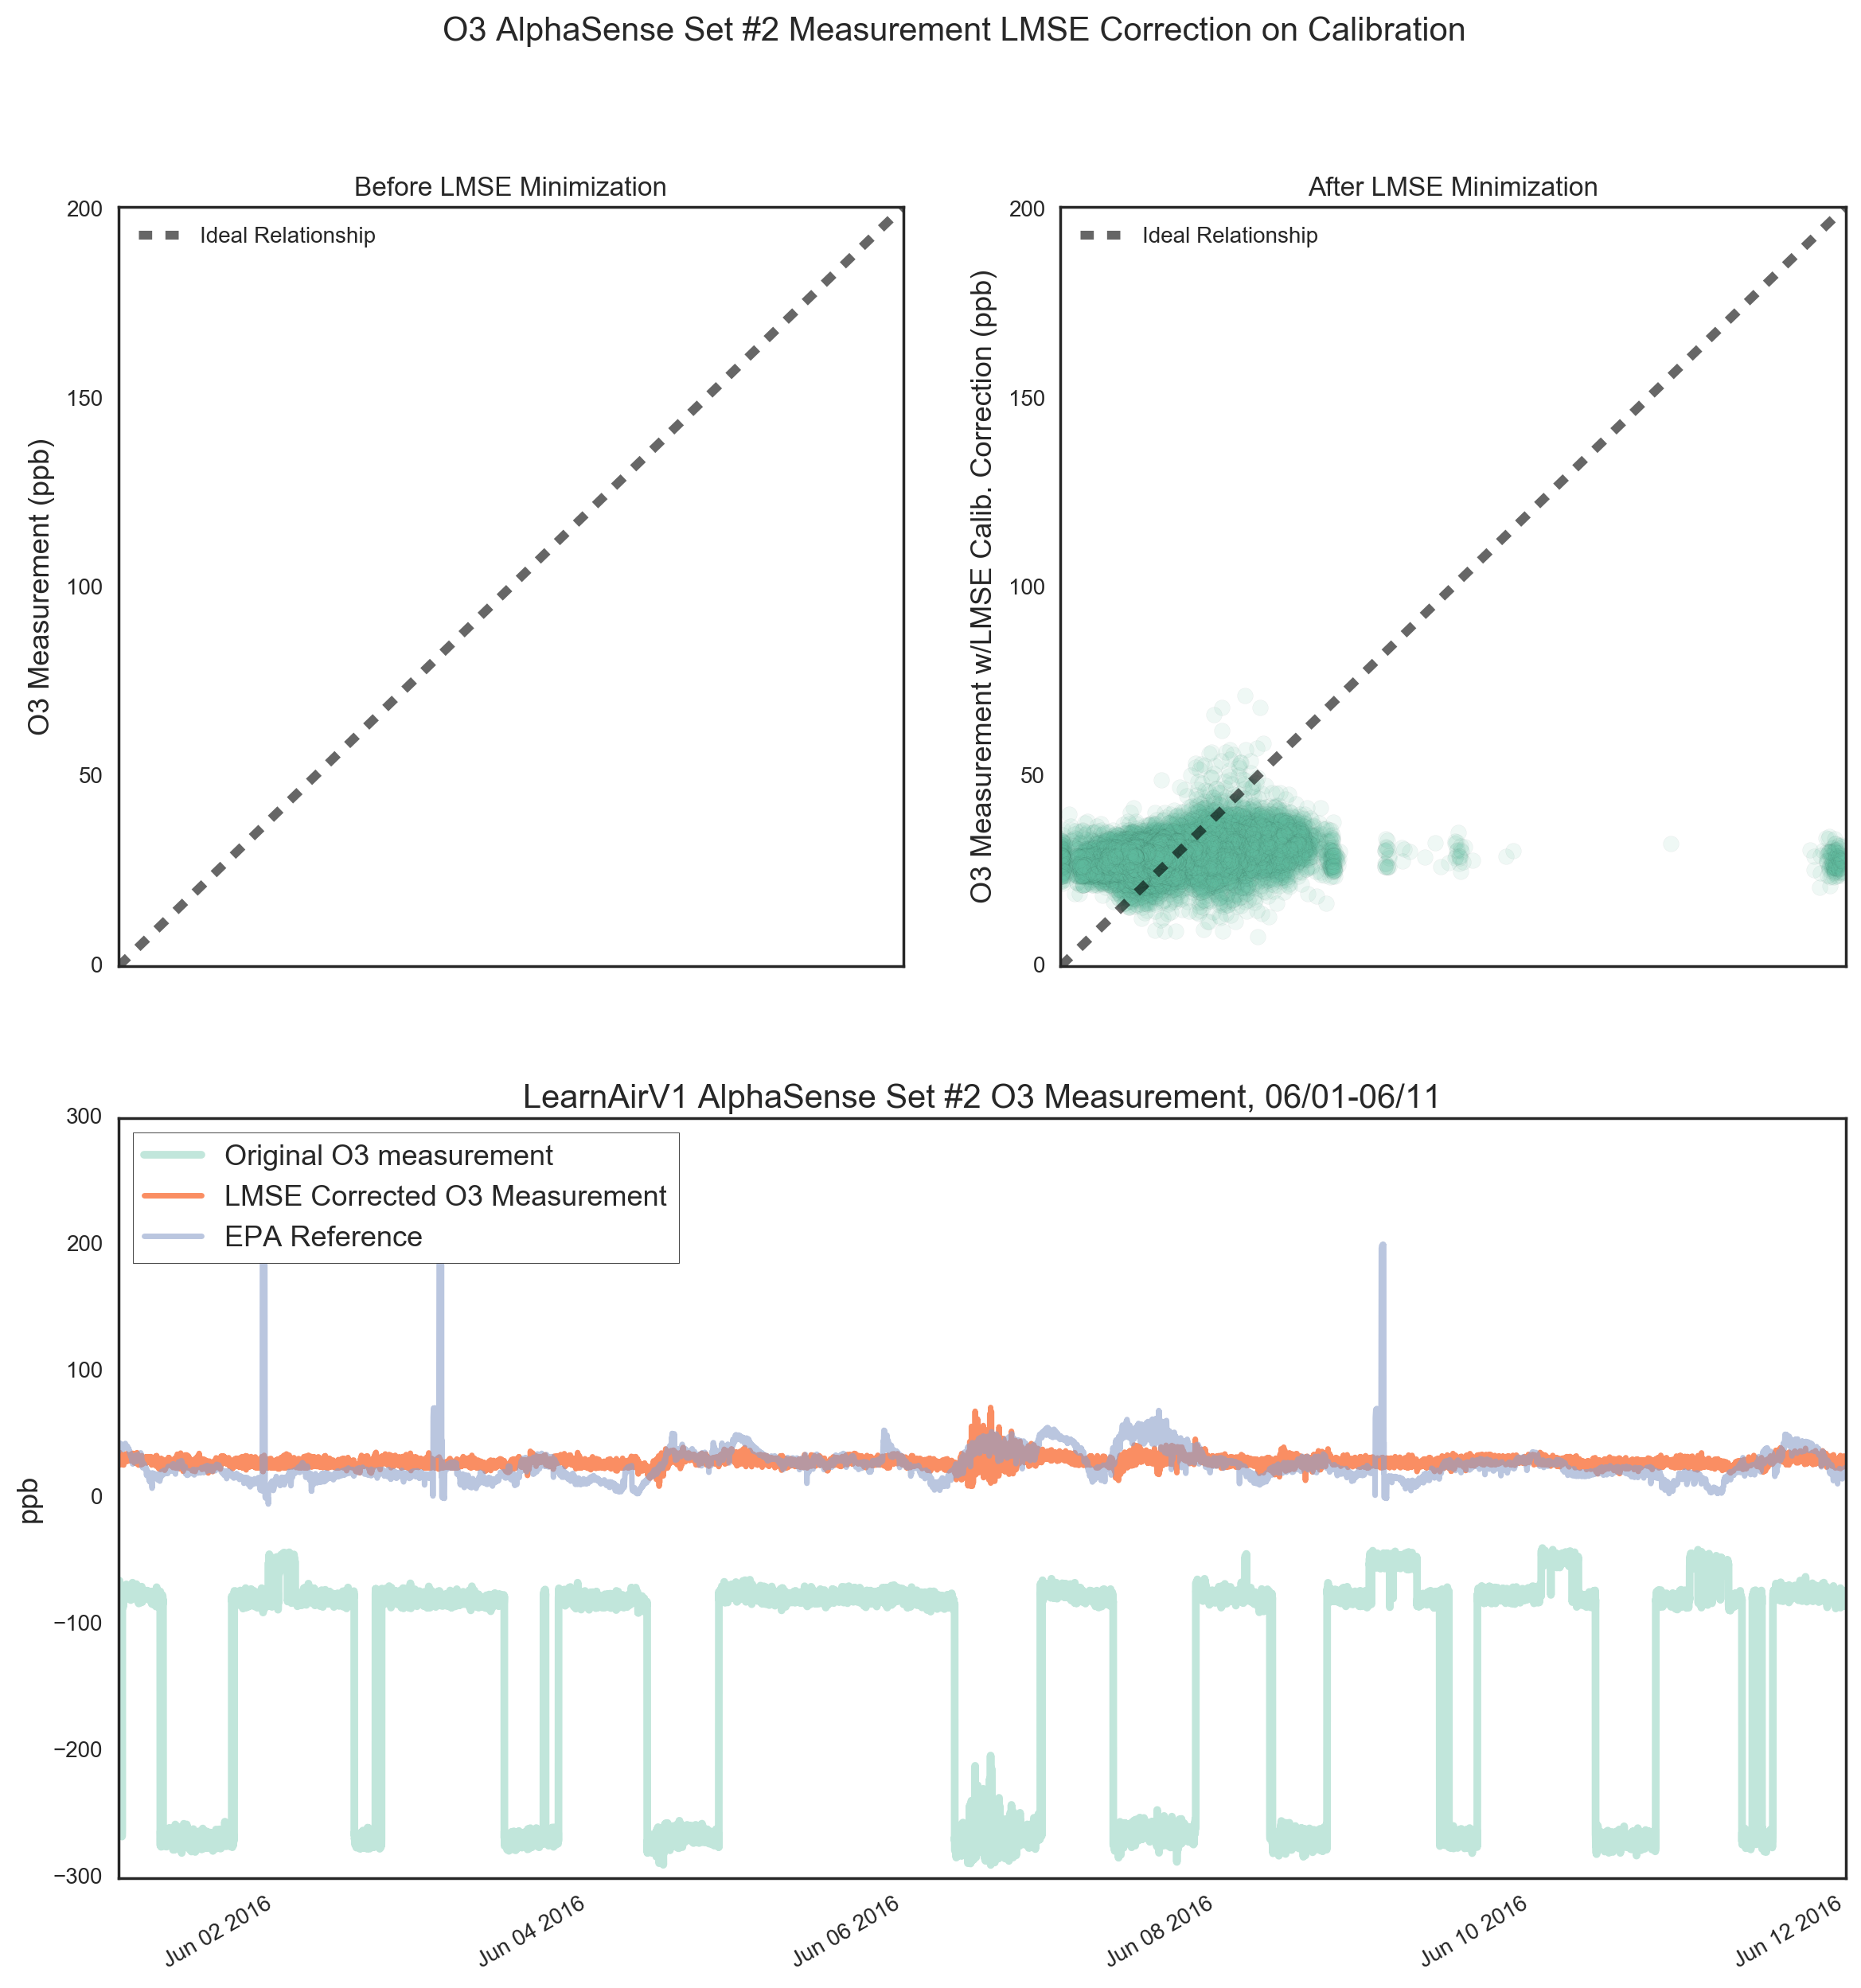
\includegraphics[width=\textwidth]{figs/as2_o3_lmse}               
 	 \caption{AlphaSense O3 Sensor #2 after LMSE Calibration}
  	\label{fig:as2_o3_lmse}
\end{figure}


\begin{figure}[htb]
 	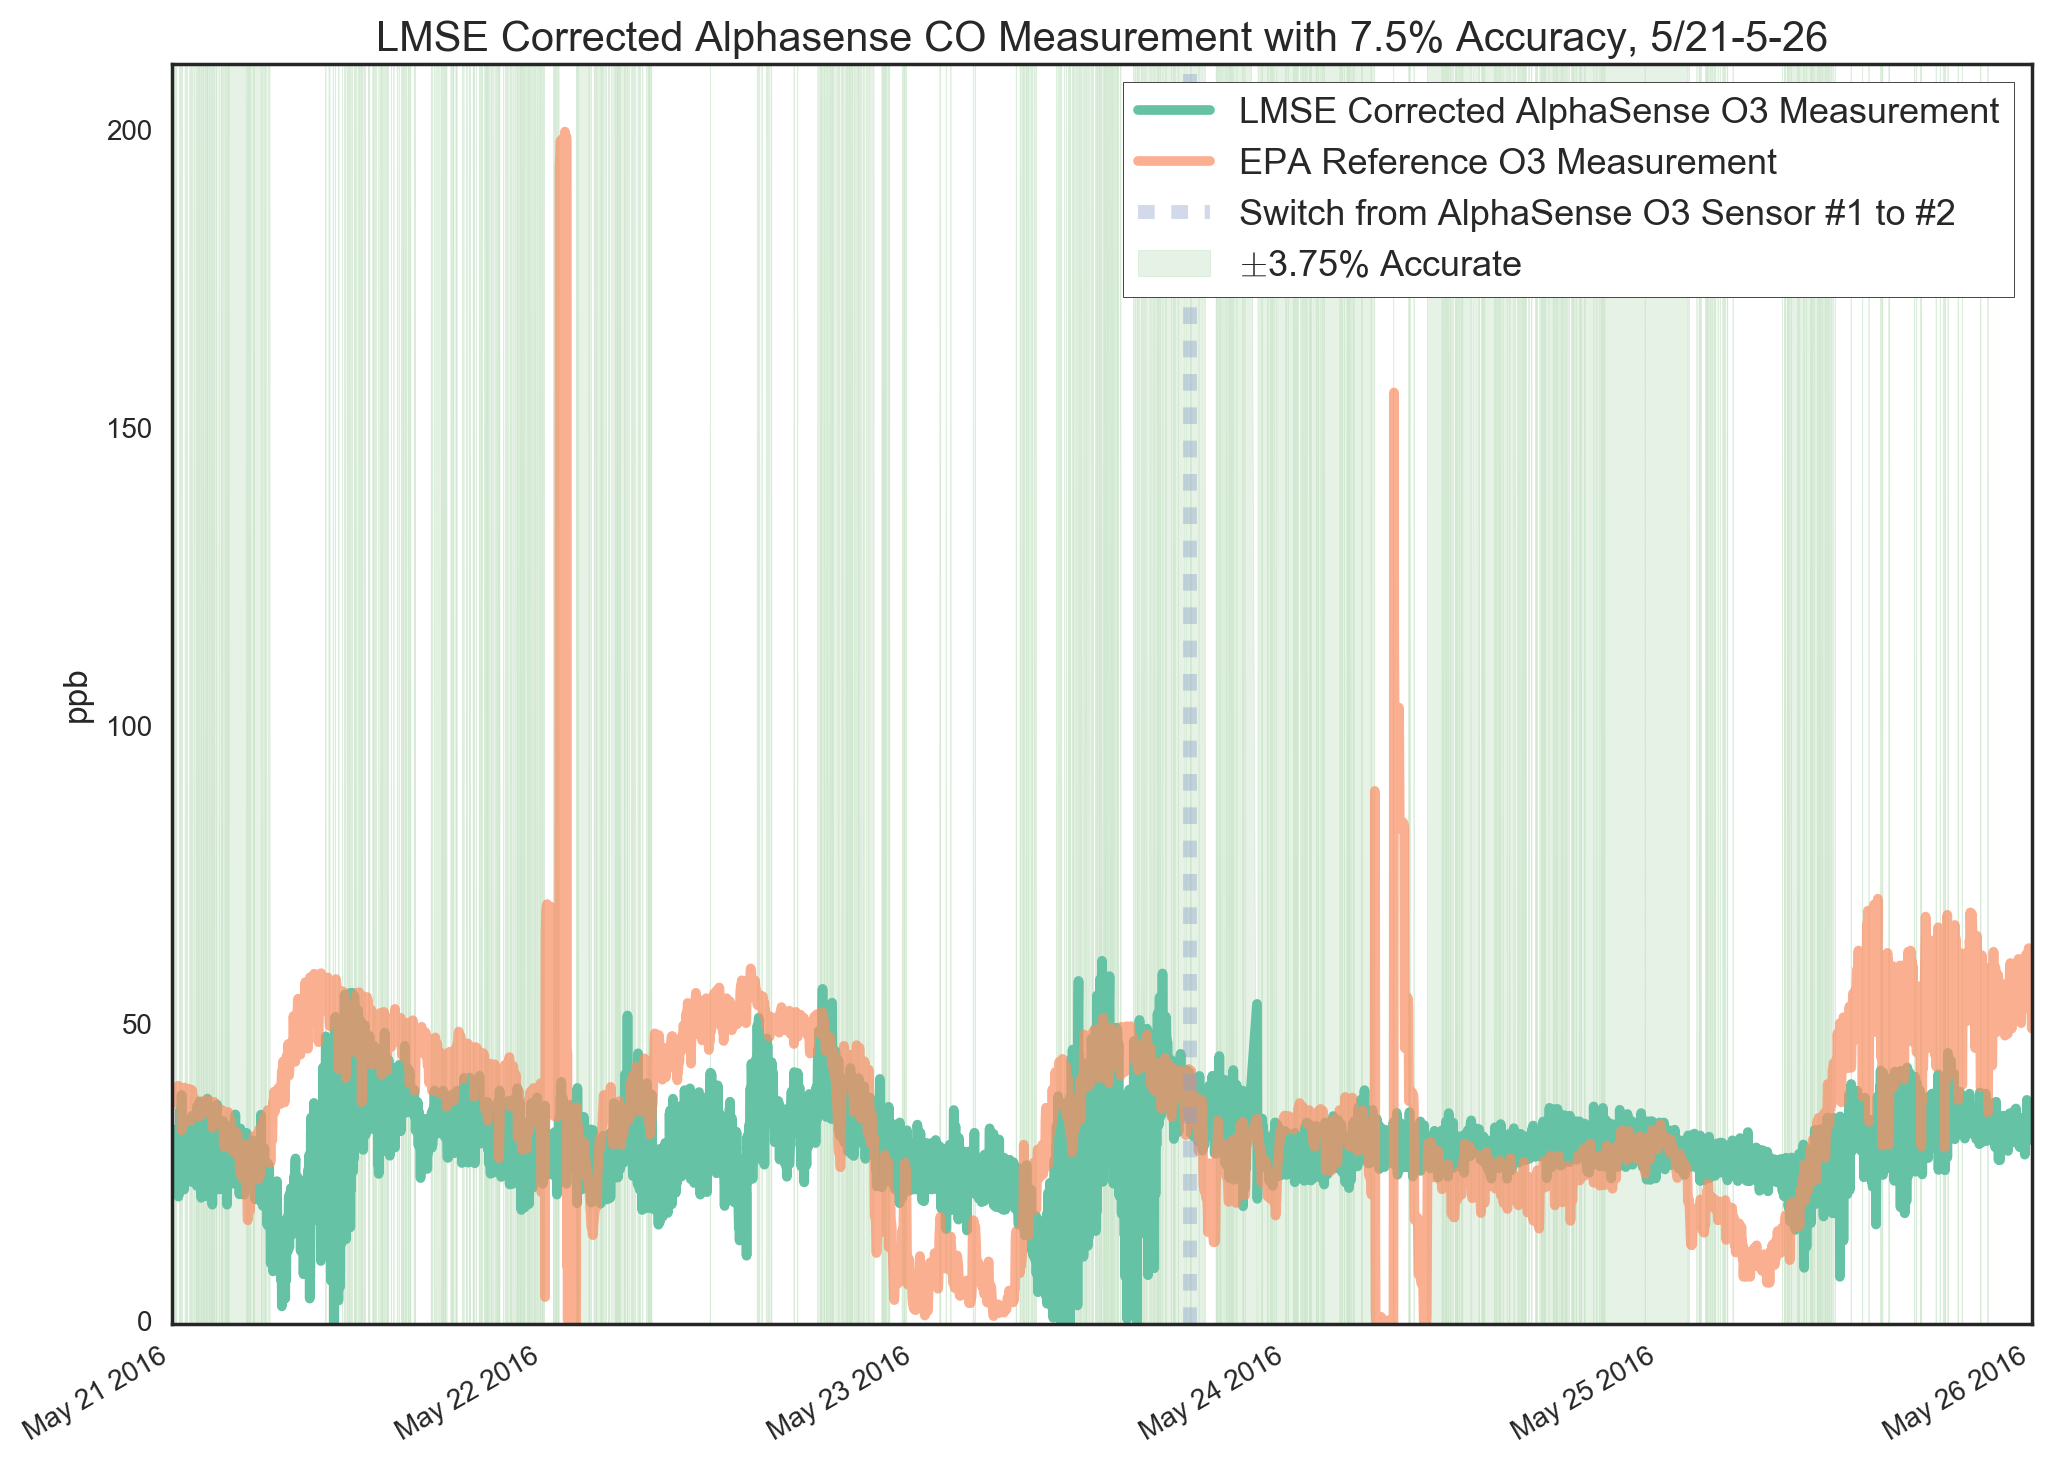
\includegraphics[width=\textwidth]{figs/as_o3_with_7p5_accuracy_zoomed}               
 	 \caption{AlphaSense O3 Sensor #1 and #2 with 7.5\% Accuracy Threshold}
  	\label{fig:as_o3_with_7p5_accuracy_zoomed}
\end{figure}


\begin{figure}[htb]
 	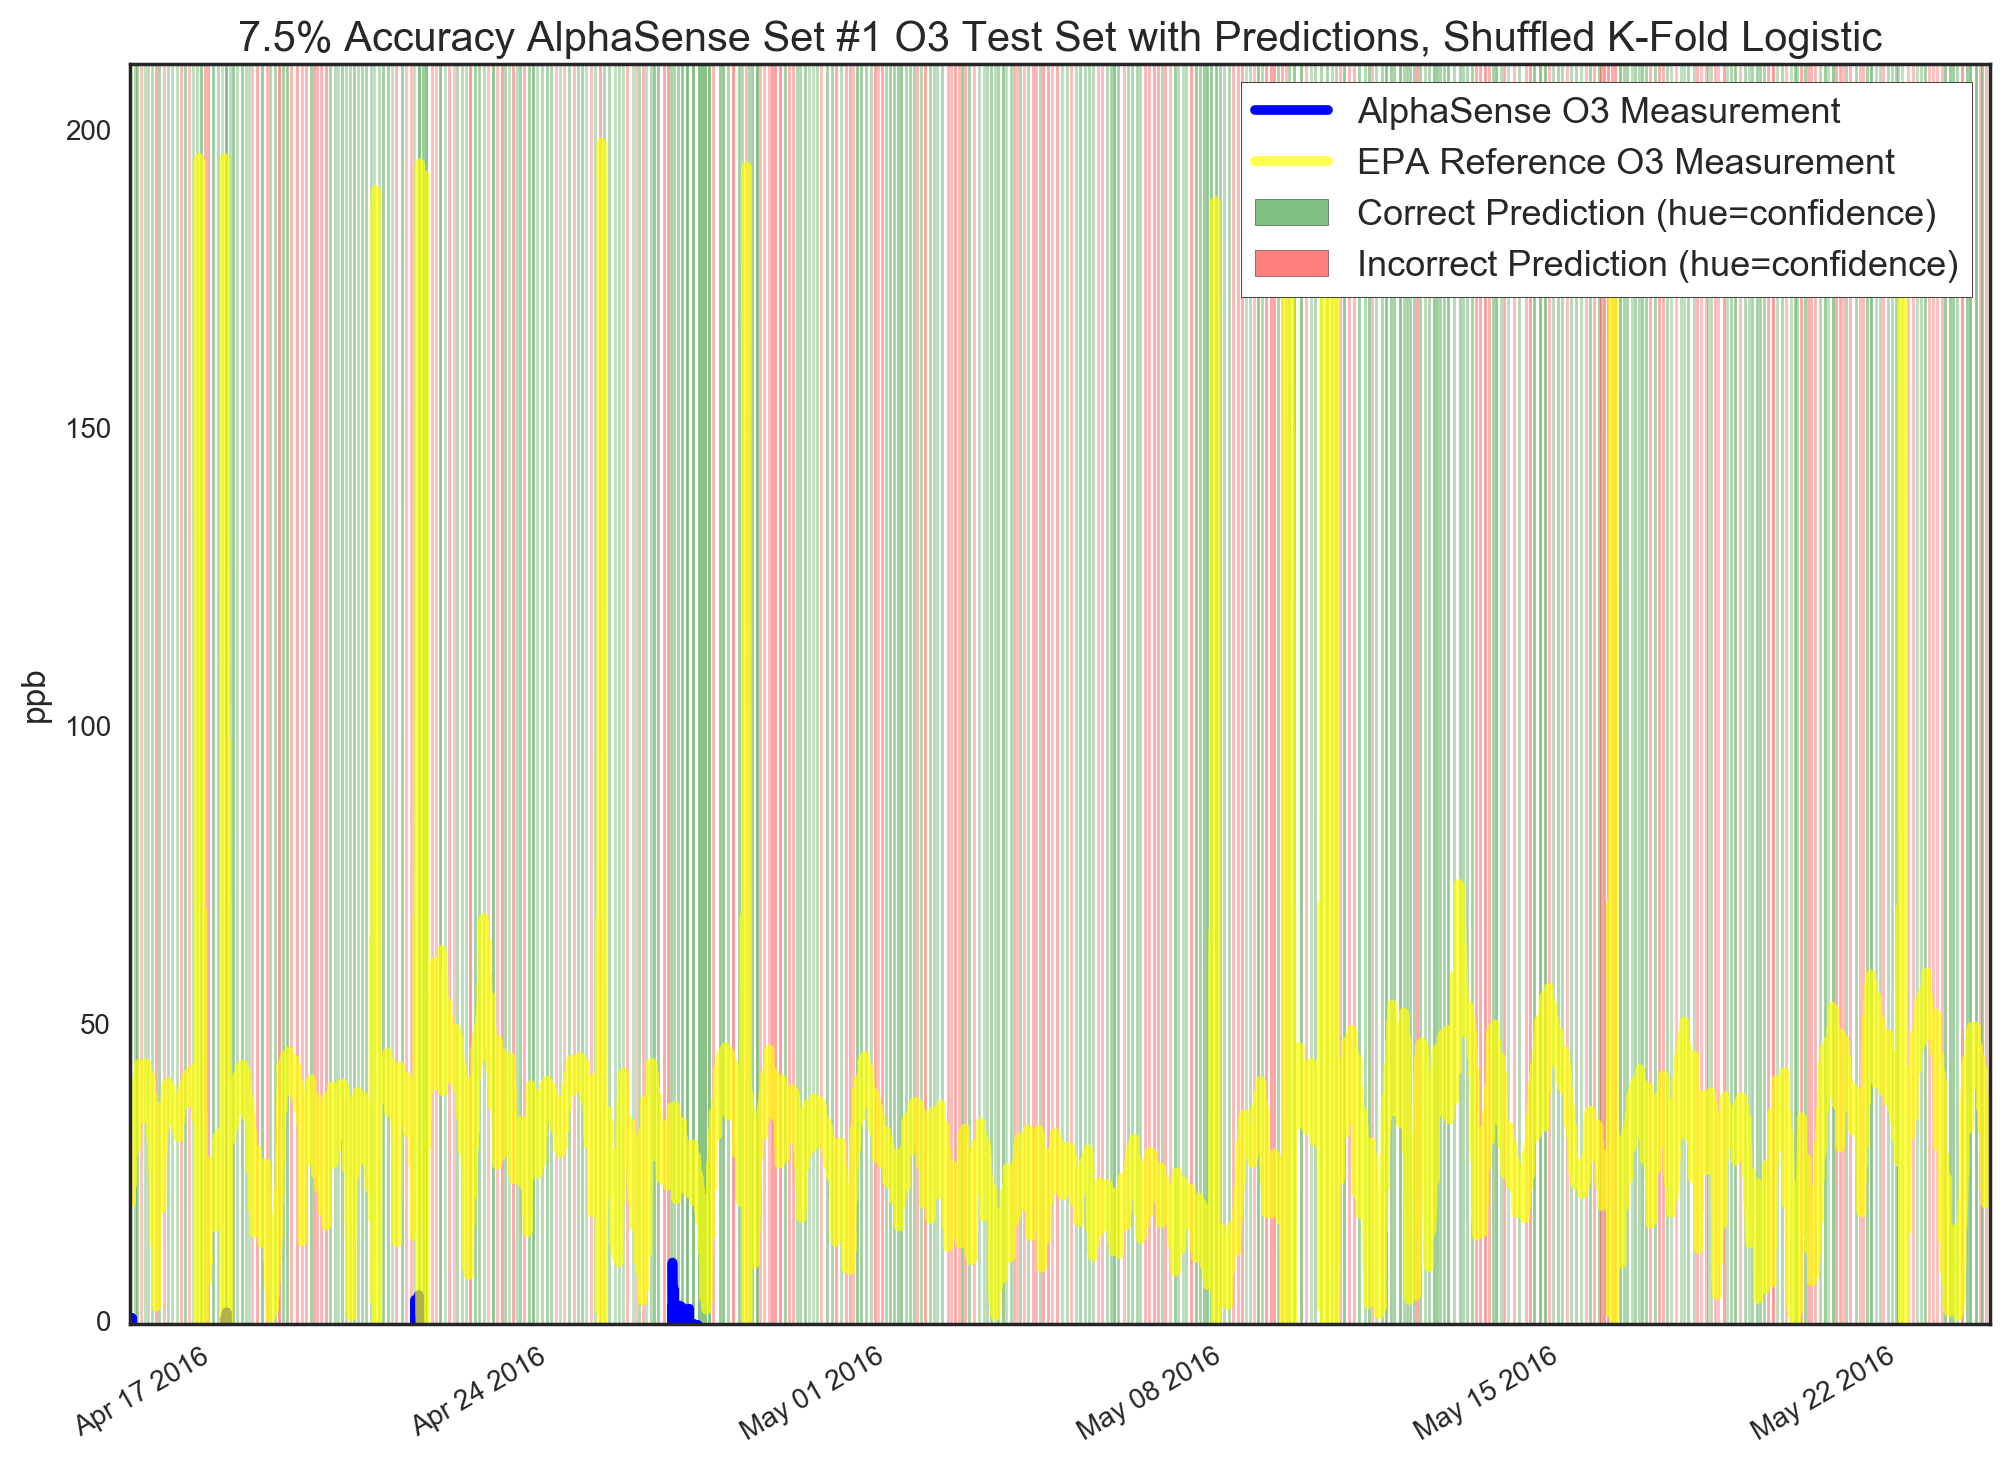
\includegraphics[width=\textwidth]{figs/as1_o3_7p5_logistic_predictions}               
 	 \caption{AlphaSense O3 Sensor #1 Prediction Accuracy}
  	\label{fig:as1_o3_7p5_logistic_predictions}
\end{figure}


\begin{figure}[htb]
 	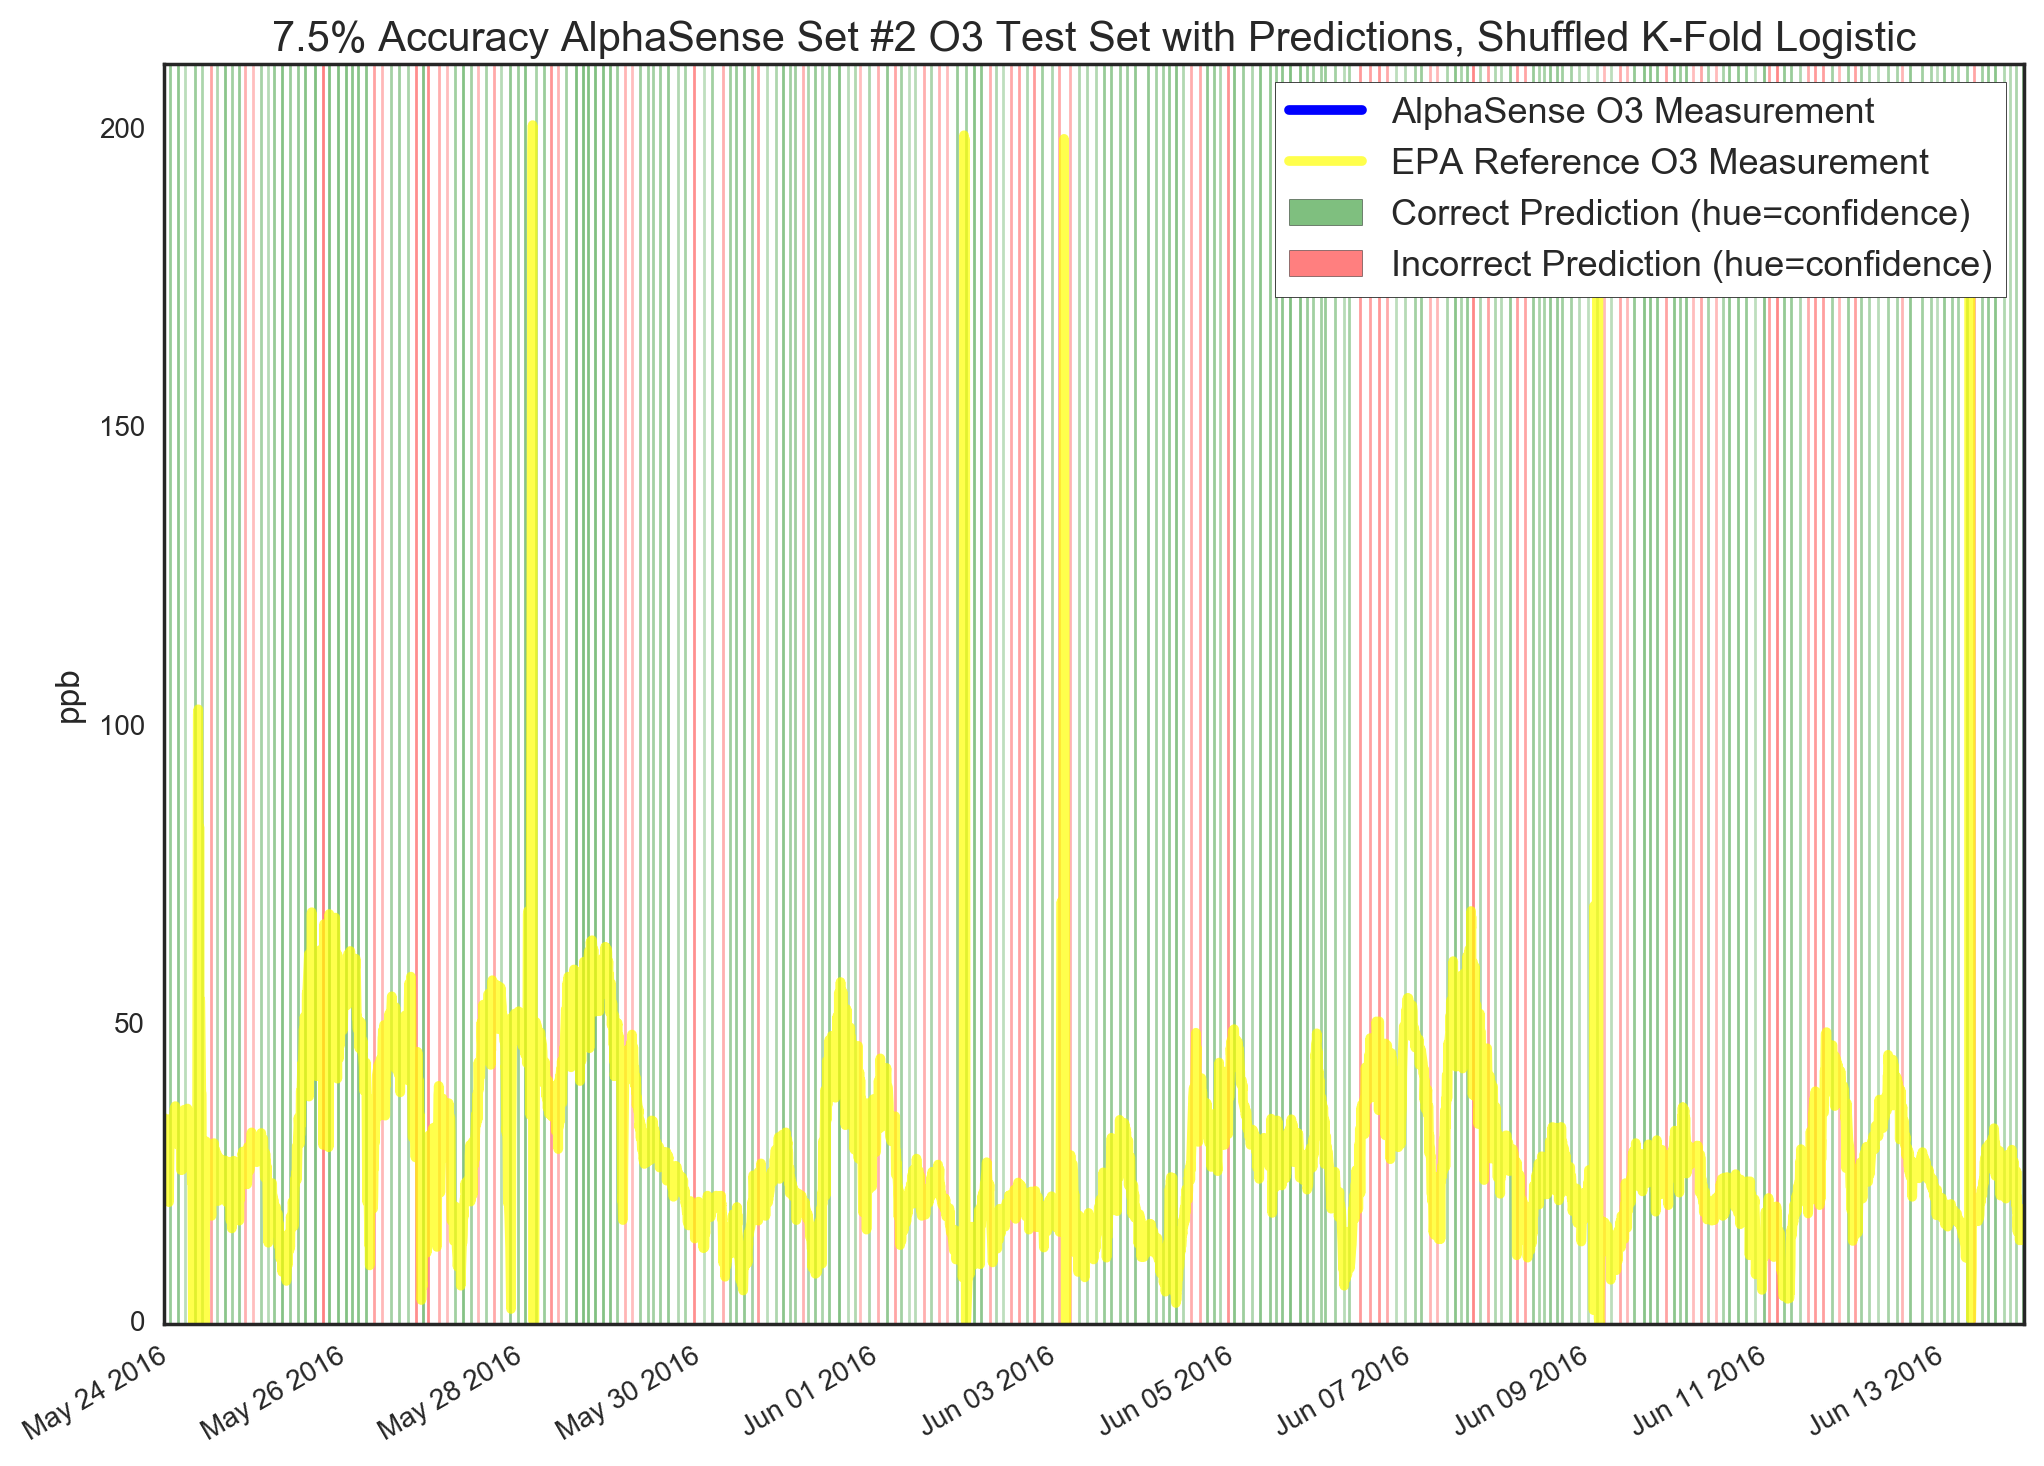
\includegraphics[width=\textwidth]{figs/as2_o3_7p5_logistic_predictions}               
 	 \caption{AlphaSense O3 Sensor #2 Prediction Accuracy}
  	\label{fig:as2_o3_7p5_logistic_predictions}
\end{figure}


\begin{table}
\centering
\small
\begin{tabular}{lclc|}
\\
\\
\toprule
Feature & Importance \\
\midrule
lmse\_calib\_as\_o3 & 0.0388052728559 \\
as\_o3 & 0.038535780326 \\
alphaS1\_work & 0.0256714422814 \\
avg\_10\_as\_o3 & 0.0143759967966 \\
avg\_10\_lmse\_calib\_as\_o3 & 0.0143305118271 \\
as\_h2s & 0.0131703607364 \\
avg\_720\_bkcarbon & 0.0131177282572 \\
avg\_60\_bkcarbon & 0.0128714271405 \\
avg\_1440\_bkcarbon & 0.0124171125826 \\
min\_since\_plugged\_in & 0.012288250826 \\
bkcarbon & 0.0122005264086 \\
avg\_1440\_lmse\_scaled\_sharpDust & 0.0118815562888 \\
avg\_720\_lmse\_scaled\_sharpDust & 0.0116399996115 \\
daily\_avg\_as\_temperature & 0.0116365039598 \\
alphaS3\_work & 0.0115947138563 \\
\bottomrule
\end{tabular}
\label{tab:as1_o3_randomforest_features}
\caption{Top 15 Features from Random Forest for O3 Sensor #1, used in Pruned Logistic Regression}
\end{table}




\begin{figure}[htb]
 	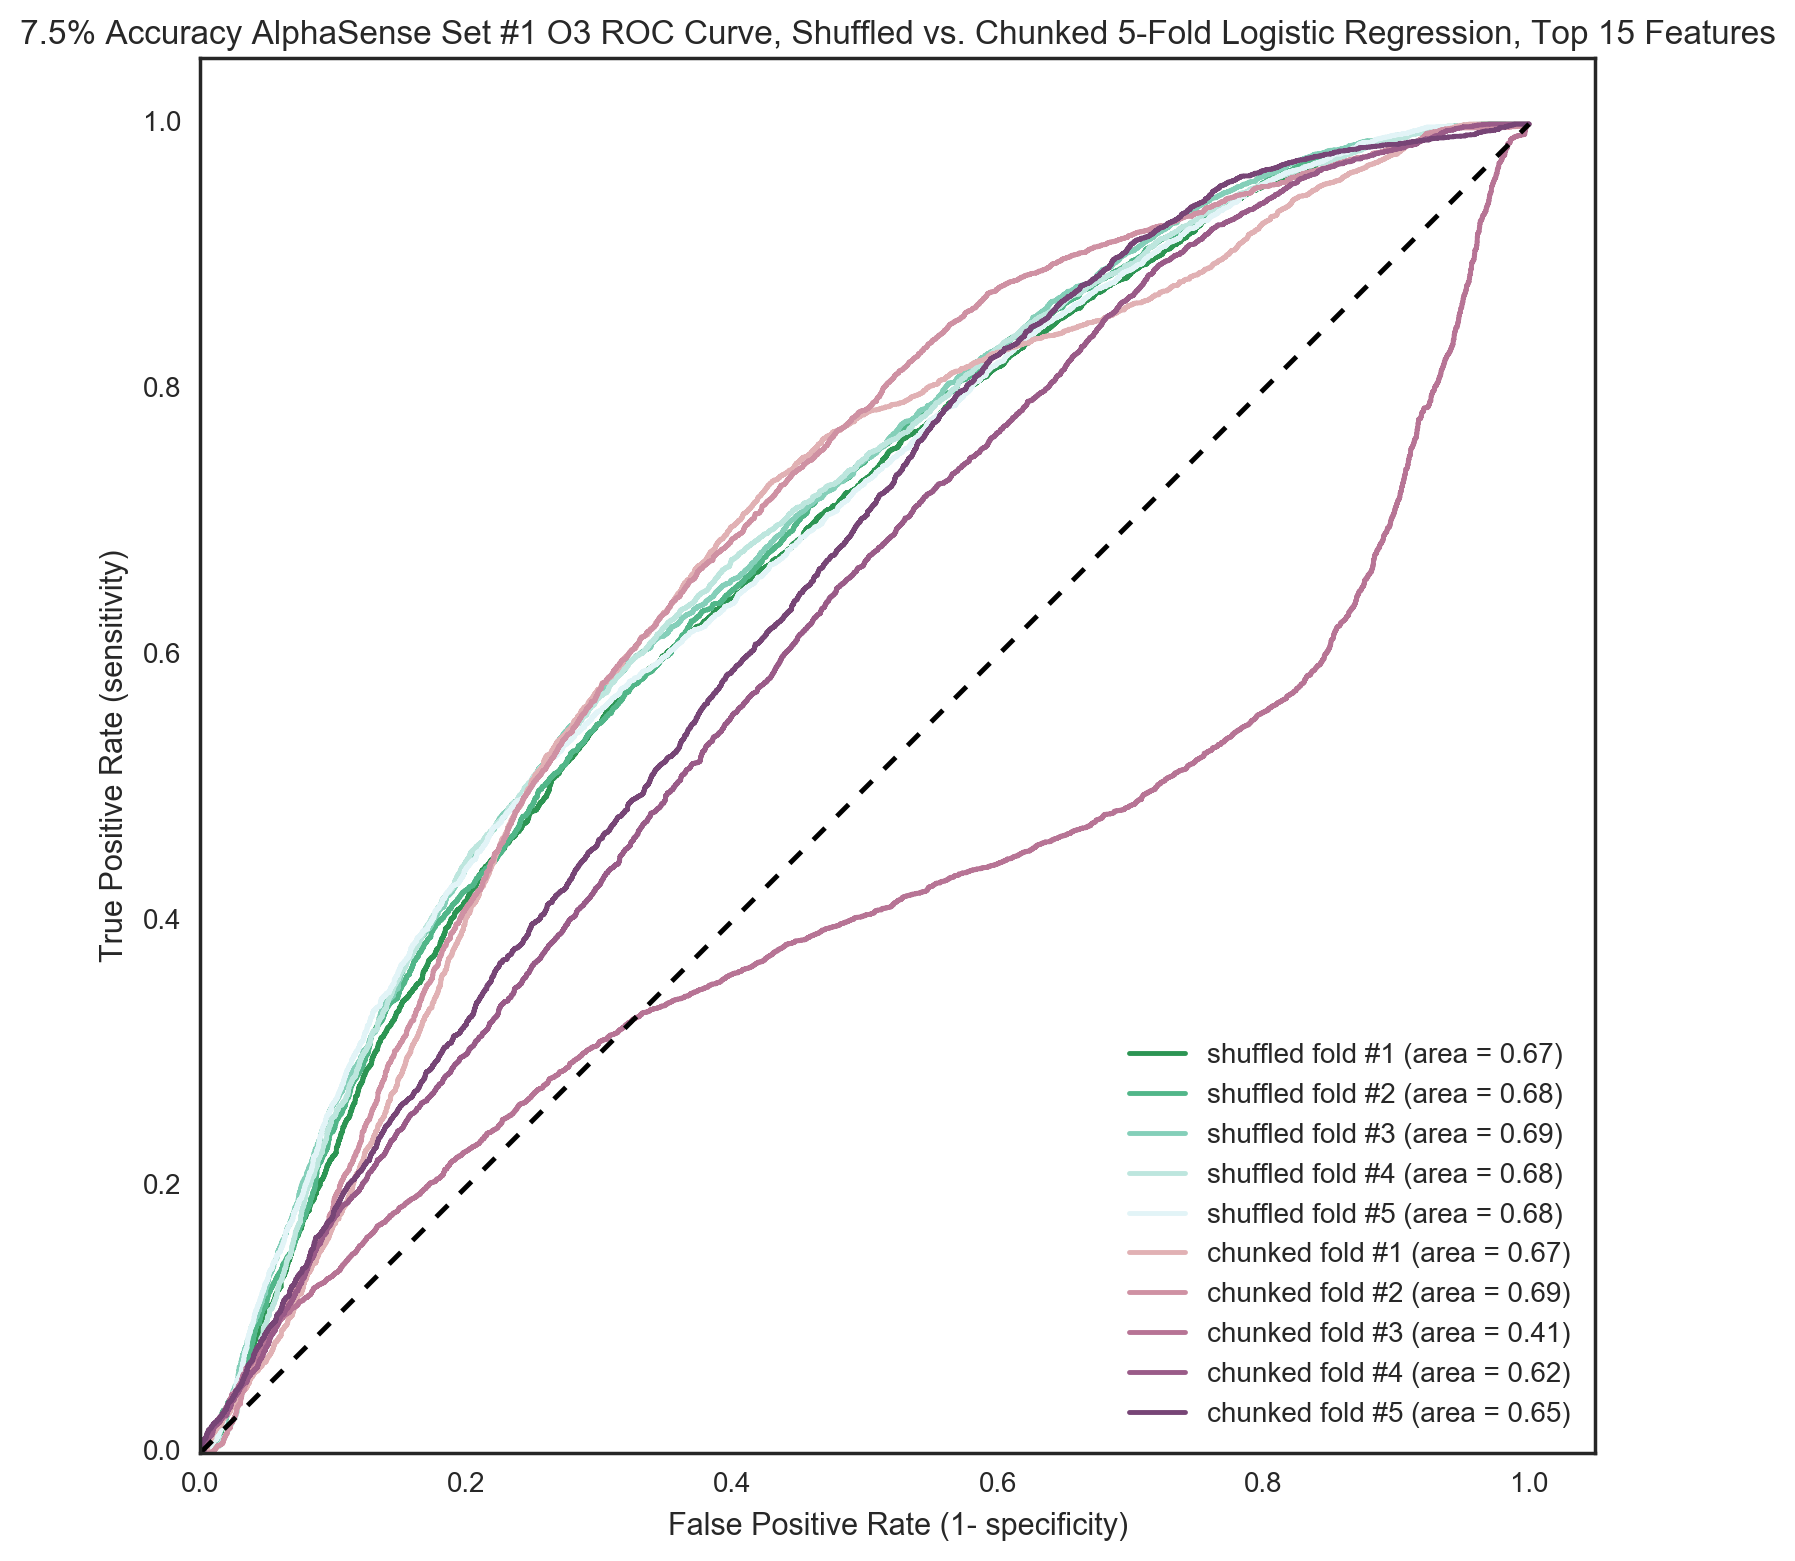
\includegraphics[width=\textwidth]{figs/as1_o3_7p5_roc_pruned_features}               
 	 \caption{AlphaSense O3 Sensor #1 ROC Using Top 15 Features}
  	\label{fig:as1_o3_7p5_roc_pruned_features}
\end{figure}



\begin{table}
\centering
\small
\begin{tabular}{lllllllll}
\\
\\
\toprule
Feature & Importance \\
\midrule
avg\_720\_bkcarbon & 0.0190323311421 \\
avg\_1440\_bkcarbon & 0.0186458328226 \\
avg\_1440\_as\_co & 0.0185435347092 \\
daily\_avg\_as\_temperature & 0.0177518437915 \\
lmse\_calib\_as\_o3 & 0.0170424373503 \\
daily\_avg\_forecastio\_temperature & 0.0170308459472 \\ 
avg\_60\_bkcarbon & 0.0167897682822 \\
min\_since\_plugged_in & 0.0166420124401 \\ 
avg\_60\_forecastio\_pressure & 0.016620265085 \\
bkcarbon & 0.015766200638 \\
daily\_avg\_forecastio\_humidity & 0.0147498428636 \\
avg\_60\_forecastio\_apparentTemperature & 0.0140509238175 \\
forecastio\_pressure & 0.013926105091 \\
avg\_60\_forecastio\_temperature_c & 0.0136171116857 \\
day\_of\_year & 0.0133242379573 \\
\bottomrule
\end{tabular}
\label{tab:as2_o3_randomforest_features}
\caption{Top 15 Features from Random Forest for O3 Sensor #2, used in Pruned Logistic Regression}
\end{table}



\begin{figure}[htb]
 	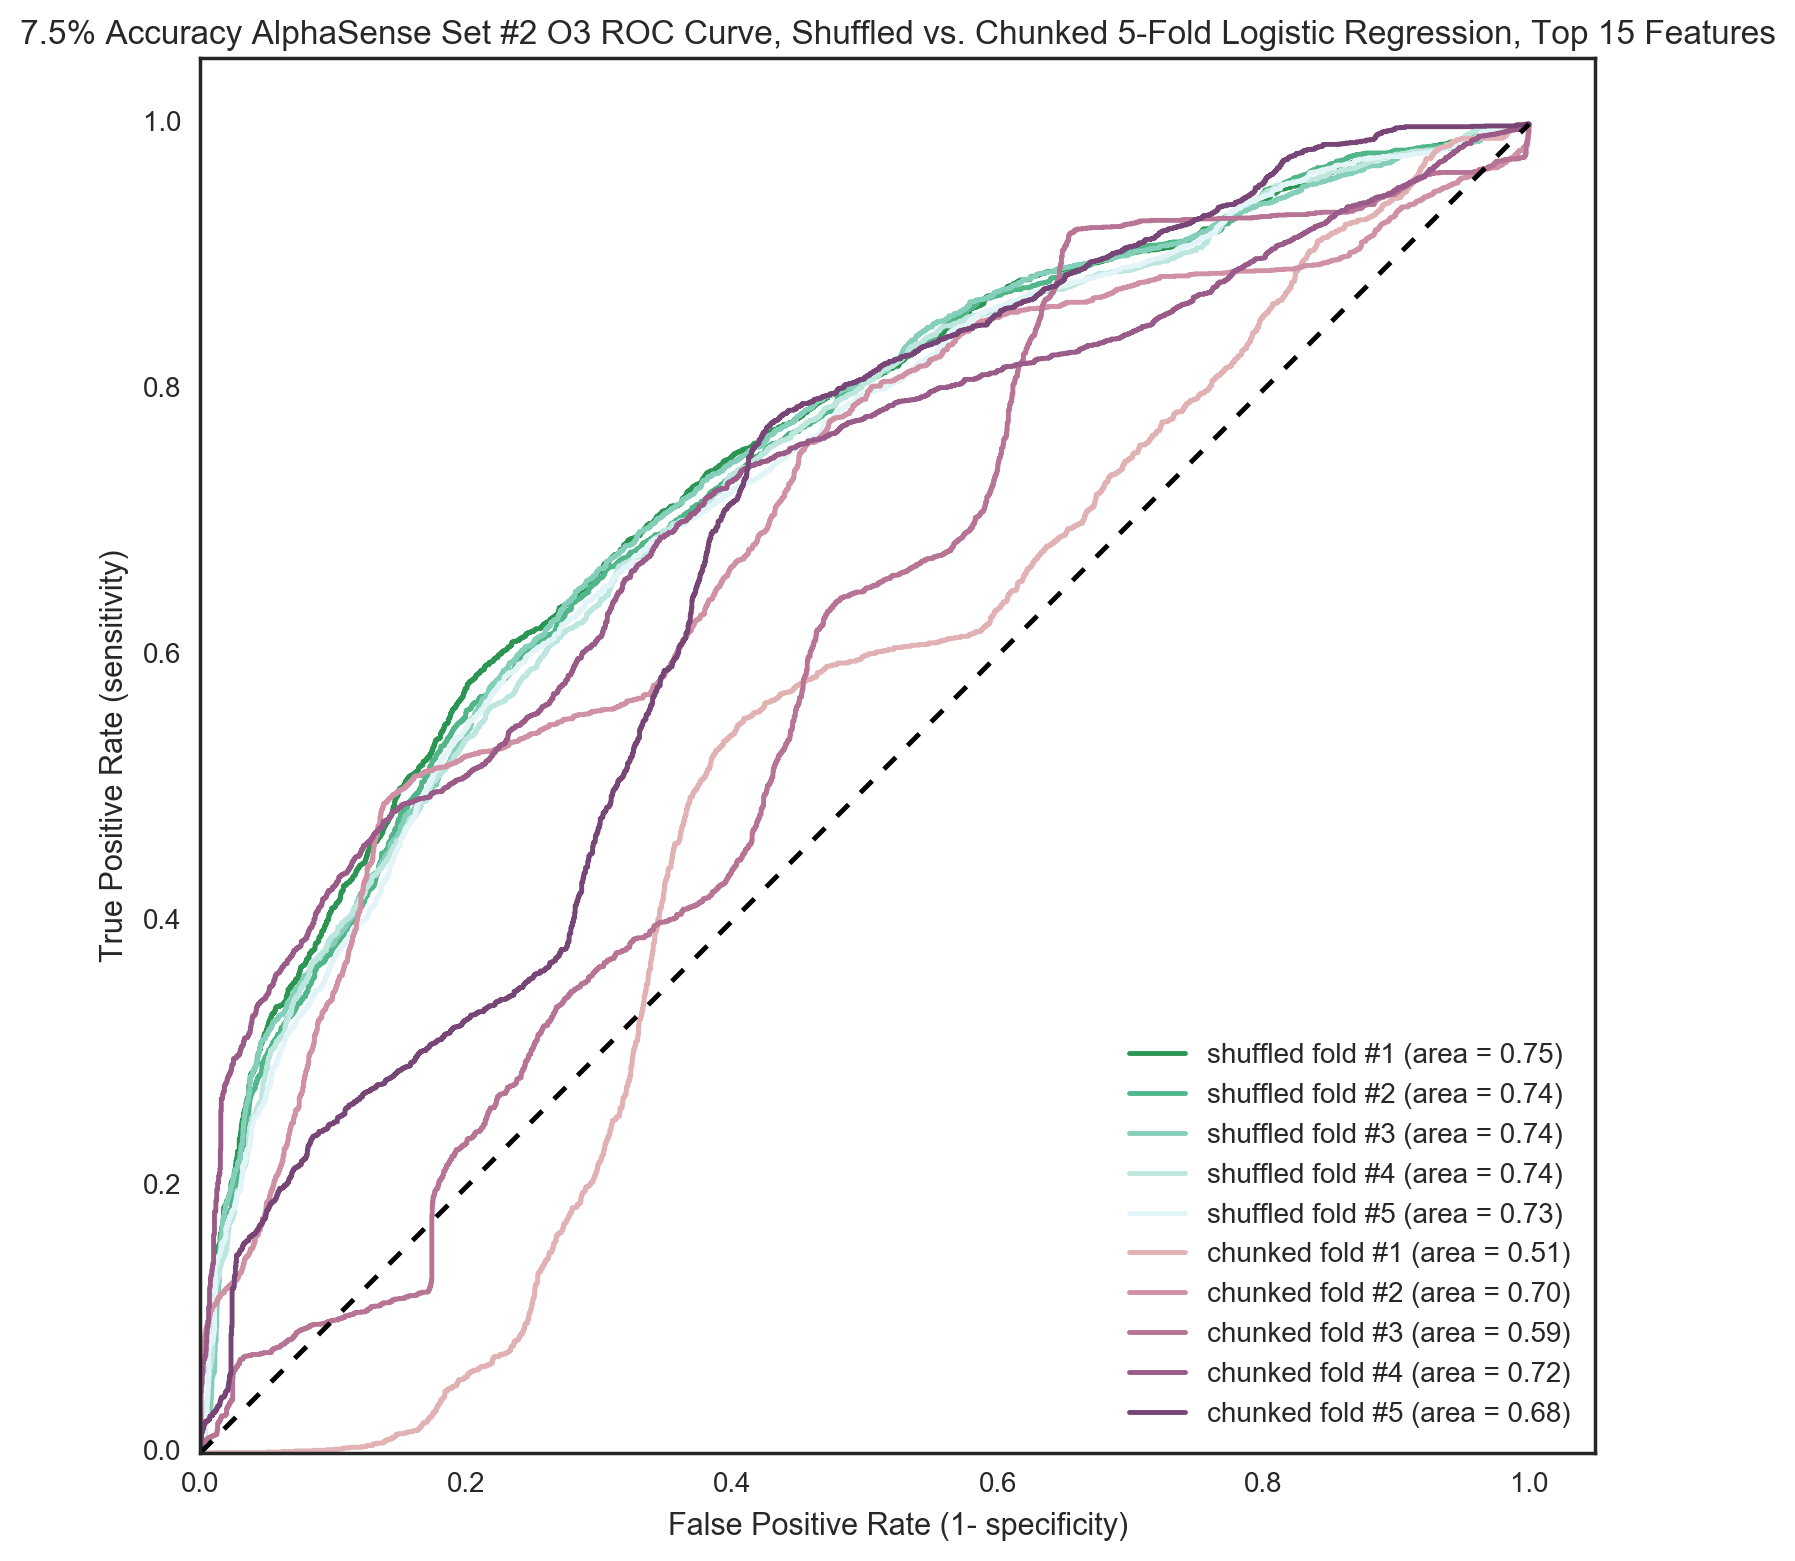
\includegraphics[width=\textwidth]{figs/as2_o3_7p5_roc_pruned_features}               
 	 \caption{AlphaSense O3 Sensor #2 ROC Using Top 15 Features}
  	\label{fig:as2_o3_7p5_roc_pruned_features}
\end{figure}


\clearpage
\newpage
